\documentclass[12pt,a4paper,twoside]{book}
\usepackage[utf8]{inputenc}
\usepackage[pctex32]{graphicx}
\usepackage{setspace}
\usepackage{emptypage}
\usepackage{float}
\usepackage{geometry}
%\usepackage[showframe]{geometry}
\usepackage{caption}
\usepackage{listings}
\usepackage{color}

\definecolor{code_comment}{RGB}{65,126,96}
\definecolor{code_keyword}{RGB}{126,8,84}
\definecolor{code_string}{RGB}{45,36,251}
\definecolor{gray}{rgb}{0.5,0.5,0.5}

\lstset{
	frame=tb,
	aboveskip=3mm,
	belowskip=3mm,
	showstringspaces=false,
	columns=flexible,
	basicstyle={\small\ttfamily},
	numbers=left,
	numberstyle=\tiny\color{gray},
	keywordstyle=\color{code_keyword},
	commentstyle=\color{code_comment},
	stringstyle=\color{code_string},
	breaklines=true,
	breakatwhitespace=true
	tabsize=3,
	captionpos=b
}

\captionsetup[lstlisting]{singlelinecheck=false,margin=0pt,font={small,sf}}
\captionsetup[figure]{singlelinecheck=false,margin=0pt,font={small,sf}}

\linespread{1.3}

% Hyphenate \texttt
\DeclareFontFamily{\encodingdefault}{\ttdefault}{\hyphenchar\font=`\-}

\begin{document}

	\frontmatter
		\begin{titlepage}
\begin{center}

\begin{Large}
	\textbf{POLITECNICO DI MILANO}\\
	Facoltà di Ingegneria\\
	Scuola di Ingegneria dell'Informazione
\end{Large}

\vspace{1.5cm}

\includegraphics[width=3cm]{imgs/poli.eps}

\vspace{1.5cm}
\begin{Large}
\textbf{
DESIGN AND DEVELOPMENT OF AN ASYNCHRONOUS DATA ACCESS LAYER FOR PERVASIVE NETWORKS
}
\end{Large}

\vfill

\begin{large}
\begin{onehalfspace}

	\begin{flushleft}
	\begin{tabbing}
	Relatore: \hspace{8pt} \= Ch.mo Prof. Ing. Fabio Alberto Schreiber\\
	Correlatore: \> Ing. Emanuele Panigati
	\end{tabbing}
	\end{flushleft}

	\vspace{1cm}
	\begin{flushright}
	\begin{tabbing}
	\hspace{300pt}
	\= Tesi di laurea di:\\
	\> GUIDO ROTA \\
	\> Matr. 819938\\
	\end{tabbing}
	\end{flushright}
	
\end{onehalfspace}
\end{large}

\vspace{2cm}
Anno Accademico 2014 - 2015

\end{center}
\end{titlepage}

		\chapter*{Sommario}
		\chapter*{Abstract}

		\tableofcontents
		
	\mainmatter
		\chapter{Introduction}

Computing devices permeate every aspect of our life. PCs, tablets, smartphones,
identification badges, credit cards, smart-watches, wearable gadgets, traffic
cameras, digital fitness bands, and personal medical devices like pacemakers or
insulin injectors are only a few of the tools that we use every day, more or
less consciously, to produce and consume information.

As the number of devices and services that surround ourselves increases, so
does the level of mutual cooperation that we expect from them. We know that our
smartphone will automatically show us the weather for our current location,
sometimes even for our hometown when we are away (How does it know where I
live? Did I ever tell it?). Navigation apps guide us through different
itineraries at different times of the day, depending on current and expected
traffic conditions. Outbreaks of the most common viral diseases can be traced
and monitored by analysing what people are searching on the web and correlating
that data with other sources like hospital records.

We have grown so accustomed to the tight level of integration between different
services and information sources, that behaviours similar to those presented
above are nowadays expected. User requirements have heightened, and products
can fail to gain traction if they don’t exploit the data that is available
around us in new and innovative ways; different computing devices and services
must discover themselves and make mutual use of the information that they
produce or consume, meshing together in what is called a Pervasive System.

Firstly envisioned by Mark Weiser \cite{weiser1991computer}, Pervasive Systems
are connected networks of independent and heterogeneous devices, whose ultimate
goal is to assist people in a way that is effectively invisible to the final
user. They are the result of a post-pc era, where scores of computing gadgets
are disseminated in our surroundings, enhancing our capabilities to sense the
world and providing ubiquitous access to information.

From a software and hardware perspective, a Pervasive Systems is a rich and
varied environment, hosting myriads of different network protocols, data
formats, and incompatible cpu architectures. Tapping the ever increasing stream
of data produced in such a heterogeneous context, and using it to build
advanced and connected products, can easily become a daunting task. Since
Weiser’s seminal paper, several endeavours have explored different techniques
for simplifying the task of building and designing Pervasive Systems, many of
    which stemmed from the research on Wireless Sensor Networks (WSN).


\section{Wireless Sensor Networks and beyond}

As suggested by the name, Wireless Sensor Networks (WSNs) are networks of
wirelessly connected devices called nodes or motes, that are able to measure or
detect physical properties from their surrounding environment. Although the
original acronym only references the sensory features of such systems, current
usage of the term WSN is commonly extended to include devices with actuation
capabilities.

Wireless Sensor Networks provide a low-cost and effective solution for
monitoring physical phenomena: several inexpensive nodes may be scattered
around the area of observation, without requiring an explicit configuration or
a wired communication infrastructure. Data is autonomously routed from the
point of origin to the interested consumers, where it is usually aggregated,
analysed and presented to the user. Flexibility and ease of deployment make
WSNs the ideal candidate for a plethora of applications, covering home
automation, theft prevention systems, healthcare, control of environmental
hazards and monitoring of production lines.

The rapid increase in popularity of WSNs, coupled with the intrinsic
difficulties of working in a variegated software and hardware environment,
spurred the development of a wide variety of frameworks, middlewares, and
ad-hoc programming languages designed for providing an easy way of access to
the functionalities offered by networks of sensing and actuating devices and
Pervasive Systems alike.

This thesis describes the design and implementation of one of these software
systems, an asynchronous data access middleware for Pervasive Networks dubbed
\textit{New PerLa Middleware}. Its history, as will be shown in
chapter~\ref{cha:perlasystem}, is strongly intertwined with the PerLa Query
Language \cite{tse_perla}, a declarative SQL-like language for collecting data
from WSNs and other distributed sensing networks. However, before delving into
the substance of this middleware, the next section will provide a short survey
on the different approaches proposed in literature for the management of
Pervasive Systems.


\section{Data management in Pervasive Systems}

Early experiences in managing sensing networks were based on ad-hoc systems
that provided bespoken solutions to specific applications. These approaches
were usually built using proprietary hardware and highly customized software
architectures, whose design was ultimately concerned with the implementation of
a limited and well-defined series of task-oriented requirements. As shown in
\cite{hartung2006firewxnet} \cite{mainwaring2002wireless}
\cite{werner2005monitoring} \cite{juang2002energy} these highly personalized
systems are poorly reuseable, since their architecture usually fails to provide
a clear separation of concerns between the pure data access mechanisms employed
to control the underlying sensing network, and the particular behaviour
required by the specific application. It soon became clear that this strategy
could not become a viable model for a simple and effective development of
pervasive applications, as all the effort and expertise put in the
implementation of such systems could not be efficiently exploited and shared in
new projects.

TinyDB \cite{madden2005tinydb} is one of the first endeavours that tried to
provide a generic abstraction suitable for the development of sensing
applications based on Pervasive Systems. A WSN managed by TinyDB is in fact
presented to the final users as a vast streaming database controlled through
SQL-like queries, which are appropriately interpreted and distributed to the
single nodes of a pervasive system in order to specify a globally coordinated
behaviour. Despite the general high-level abstraction employed by this system,
the execution of TinyDB queries requires all nodes in the sensing network to be
running TinyOS \cite{levis2005tinyos}, an embedded operating system
specifically designed to be used in sensing devices, therefore limiting the
variety of devices which can be managed using this approach.

Similarly to TinyDB, DSN \cite{chu2006entirely} aims at providing a
database-like abstraction of an entire Pervasive System, which can be queried
and controlled using a Datalog dialect dubbed Snlog. A comparable ``WSN as a
database'' abstraction, as will be shown in chapter~\ref{cha:perlasystem}, is a
characteristic feature of the PerLa System as well.

Other projects tried to approach the problem of handling a Pervasive System by
shifting the focus on the management of highly heterogeneous networks of
sensing devices. SWORD \cite{sword} tries to achieve this goal by providing a
central infrastructure that can be used to monitor events and signals collected
from a distributed mesh of nodes. Unfortunately, its XML-over-HTTP messaging
system considerably reduces the variety of devices that can be integrated. GSN
\cite{aberer2006global}, on the other hand, is a Java Middleware based on the
concept of \textit{Virtual Sensor}, a high-level software component aimed at
providing a common interface that can be used to collect information generated
by a single device of a sensing network. Virtual Sensors are created by means
of a declarative XML descriptor, and can be interfaced with the remote
endpoints through a specific device driver dubbed \textit{wrapper}.
Unfortunately GSN does not provide any mechanism for automating the deployment
of new Virtual Sensors.

The TinyREST \cite{luckenbach2005tinyrest} project attempts to provide a
RESTful \cite{fielding2000architectural} data access interface to each node
available in a Pervasive System. This goal is achieved through a server
infrastructure that performs a mapping between HTTP methods and various
Input/Output operations performed by the devices of a sensing network. As a
result, an HTTP GET request can be used to sample a physical phenomena, whereas
a PUT operation allows users to command actuators or set variables on remote
devices. Its reliance on the TinyOS makes it vulnerable to the same critiques
made to TinyDB.

Contiki \cite{dunkels2004contiki} is a lightweight and portable operating
system specifically designed for memory-limited devices. Differently from
TinyOS, Contiki tries to foster the same programming model available to desktop
machines. Its kernel, whose footprint may ary between 10 and 30 KB of RAM,
provides in fact a fully functional IPv4 and IPv6 networking stack, a
multi-thread concurrency mechanism based on protothreads and an over-the-air
programming mechanism. Differently from the other projects discussed in this
section, Contiki does not provide any high-level abstraction for accessing the
information produced by a Pervasive System.

		\chapter{The PerLa System}

PerLa is a software infrastructure for data management and integration in
Pervasive Information Systems. Its development began in 2005 at Politecnico di
Milano, with a thesis by Marco Marelli and Marco Fortunato entitled ``\textit{A
Declarative Language for Pervasive Systems}'' \cite{mm_thesis}. With this
document the two authors laid the foundations of a completely declarative,
SQL-like language that could be used to gather information from Pervasive
Systems and Wireless Sensing Networks. Though their work primarily focussed on
defining the syntax and semantics of the PerLa language, Marelli and Fortunato
went on to propose a reference software architecture that could support the
execution of PerLa data collection queries.

In their first design they envisioned the possibility of creating a
\textit{Device Access Layer} whose goal was to conceal all the idiosyncratic
features of a Pervasive System, and provide a homogeneous data access interface
that could be used as a thought device to support the first development stages
of PerLa. The principal element of this earliest software architecture was the
\textit{Logical Object}, a virtualization module that provides a uniform API
for accessing the functionalities of a single device in the sensing network.
This germinal architecture evolved during the course of the following years
into what would later be known as \textit{PerLa Middleware}. 

The PerLa Middleware~\cite{tse_perla} was primarily concerned with providing an
actual implementation to the Logical Object abstraction, a goal that was
achieved with the creation of the Functionality Proxy Component (\texttt{FPC}).
The \texttt{FPC} is a Java entity that reifies all concepts embodied by the
Logical Object, with particular emphasis on the ability to abstract the
peculiar features of a single sensing device through a common and uniform
programming interface. The PerLa Middleware, however, was more than a simple
implementation of the Logical Object, as it provided a \textit{Plug \& Play}
system for the autonomous creation of \texttt{FPC} objects and an initial
release of the PerLa Query Executor component.

The development of the PerLa Middleware has been a collaborative effort that
involved multiple students and several years of work. The product that was
created is thus the sum of all contributions made by different people, that, at
one time or another, put their minds and hearts at the design and
implementation of the system. While this development methodology allowed PerLa
to thrive and mature rapidly, since many intellects had the possibility to
contribute with their innovative ideas, it also meant that its growth has been
dishomogeneous and, at times, chaotic. It is under these premises that, in
early 2014, the Middleware underwent a complete redesign, whose primary
intentions were to consolidate the main programmatic API (Application
Programming Interface), improve performances, and further advance some of the
defining characteristics of the system. This thesis is a description of this
recent endeavor, and will continue by describing the past, present and
foreseeable future of the PerLa System.

The remaining sections of this chapter provide an account of PerLa prior to the
current redesign, starting with the previous Middleware architecture --- also
known as Classic PerLa Middleware --- and ending with a short digression
towards Context management in Pervasive Systems. This same chapter will
describe the main features of the PerLa Query Language, which as of today still
is the interface of choice for using PerLa.
Chapters~\ref{cha:middleware_overview} and~\ref{cha:components} contain an
in-depth description of the New Middleware architecture, which should be of
concern to any programmer interested in developing new PerLa Plugins or
connecting new types of sensing devices. Finally, chapter~\ref{cha:conclusions}
wraps up the work illustrated in this thesis, and provides an outlook on the
prospects for PerLa's future.


\section{The Classic Middleware Architecture}

As stated in the previous sections of this chapter, the principal element of
the PerLa Middleware, both in its classic and redesigned incarnations, is the
\texttt{FPC}. Its primary function consists in providing a consistent and
homogeneous interface that can be used by high-level components of the PerLa
System to access all functionalities of a Pervasive System, without requiring
any knowledge of the underlying hardware layer.

\begin{figure}[h!]
\center
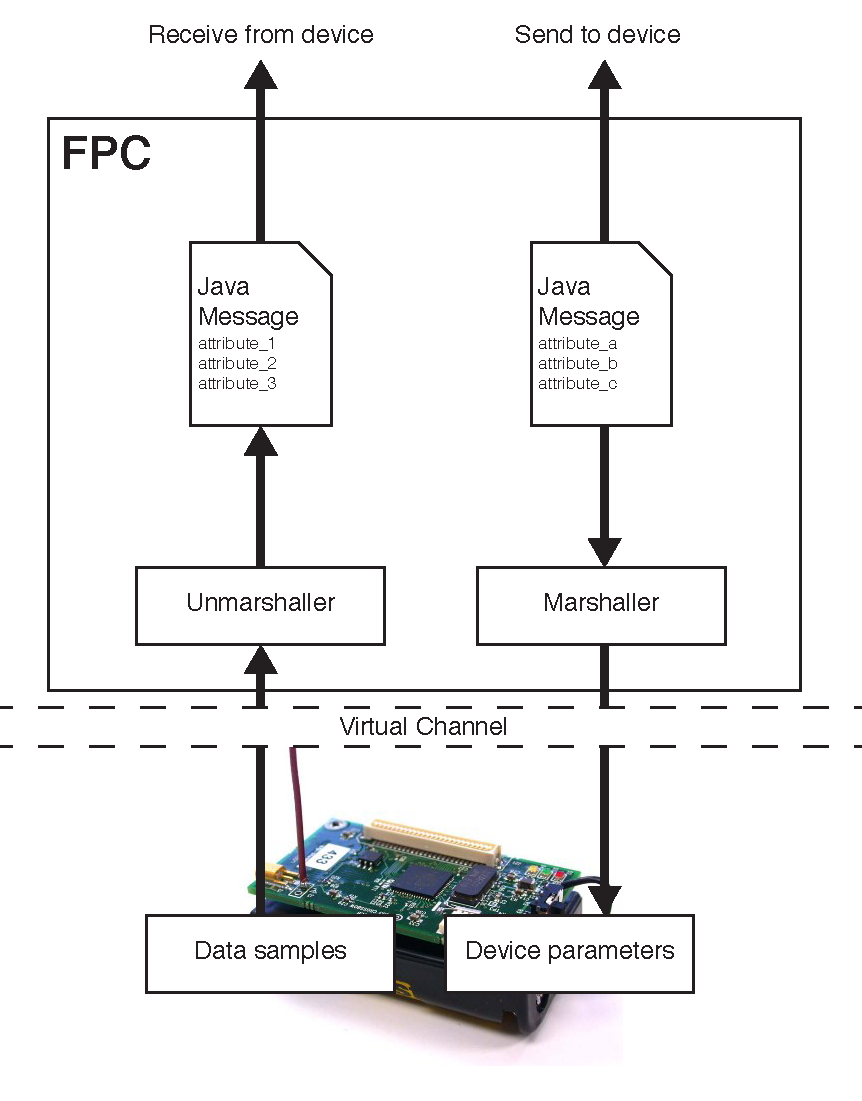
\includegraphics[width=0.6\textwidth]{imgs/classic_fpc.pdf}
\caption{The Classic FPC design}
\label{fig:classic_fpc}
\end{figure}

All data elements accessible through an \texttt{FPC} are abstracted using the
concept of \textit{Device Attribute}, namely a single piece of information
produced or consumed by a node in the Pervasive System. By design, device
attributes are not tied to a particular technology, and can therefore be used
to represent any primitive value, regardless of the method employed for its
generation (physical sampling, read from main memory, etc.). Device Attributes
are one of the defining aspects of the PerLa Middleware, as any operation
performed through the \texttt{FPC} interface has to be specified in terms of
reading or writing a specific set of attributes.

\begin{figure}[h!]
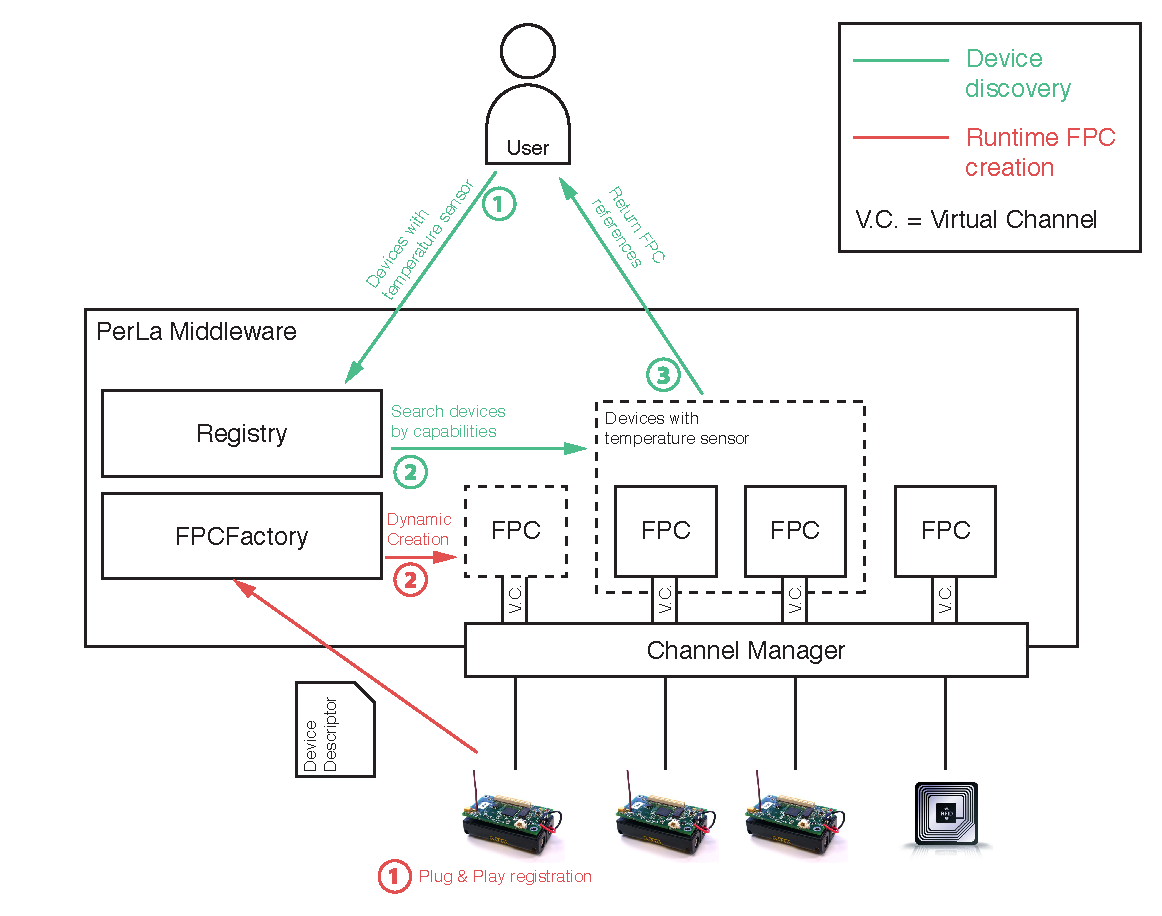
\includegraphics[width=\textwidth]{imgs/classic_middleware_overview.pdf}
\caption{The Classic PerLa Middleware architecture}
\label{fig:classic_architecture}
\end{figure}

In the Classic PerLa Middleware, the physical connection between an
\texttt{FPC} and its remote device is entirely managed by the \texttt{Channel
Manager} (see figure~\ref{fig:classic_architecture}). This component is
responsible for the creation of \texttt{Virtual Channels}, abstract network
interfaces that conceal the specific technologies required to hold a
communication link between two endpoints of a Pervasive System. By means of the
\texttt{Channel Manager}, \texttt{FPC}s and physical devices can exchange
information transparently, mutually ignoring all the differences that may exist
between them; The achievement of this goal, however, is strictly limited by the
capabilities of the \texttt{Channel Manager} itself, as the choice of protocols
available in the Classic Middleware is restricted to those that the original
PerLa Developers hard-coded into this component.

Sensing nodes can be added to a running instance of the PerLa Middleware
through a \textit{Plug \& Play} device registration mechanism. This operation
is performed at runtime by the \texttt{FPCFactory}, a software component tasked
with creating new \texttt{FPC} objects from a blueprint document called
\textit{Device Descriptor}. PerLa-enabled devices are programmed to send their
XML descriptor at startup; this allows them to be readily available for use, as
their controlling \texttt{FPC} object is dynamically instantiated by the
\texttt{FPCFactory} upon reception of the Device Descriptor.

As shown in figure~\ref{fig:classic_fpc}, the internal structure of the Classic
\texttt{FPC} is mainly composed of a \texttt{Marshaller}, an
\texttt{Unmarshaller}, and a selection of Java objects representing the
messages which can be exchanged with the remote endpoint. This early design is
enough to implements a simplified data collection mechanism, based on the
assumptions that every device attribute can be mapped to exactly one message
field. Under the Classic Middleware, a typical data collection request for a
well-defined set of attributes would then be executed as follows:

\begin{enumerate}

    \item Starting from a user's request, and leveragin the one-to-one
        relationship between attributes and message fields, the \texttt{FPC}
        compiles a list of data structures which are to be collected from the
        remote device;

    \item The remote device starts streaming data to the \texttt{FPC}. This
        information is unmarshalled into a high-level Java message, according
        to the directives specified inside the Device Descriptor;

    \item All message fields containing relevant information for the user are
        read in order to produce an output record.

\end{enumerate}

\begin{figure}[h!]
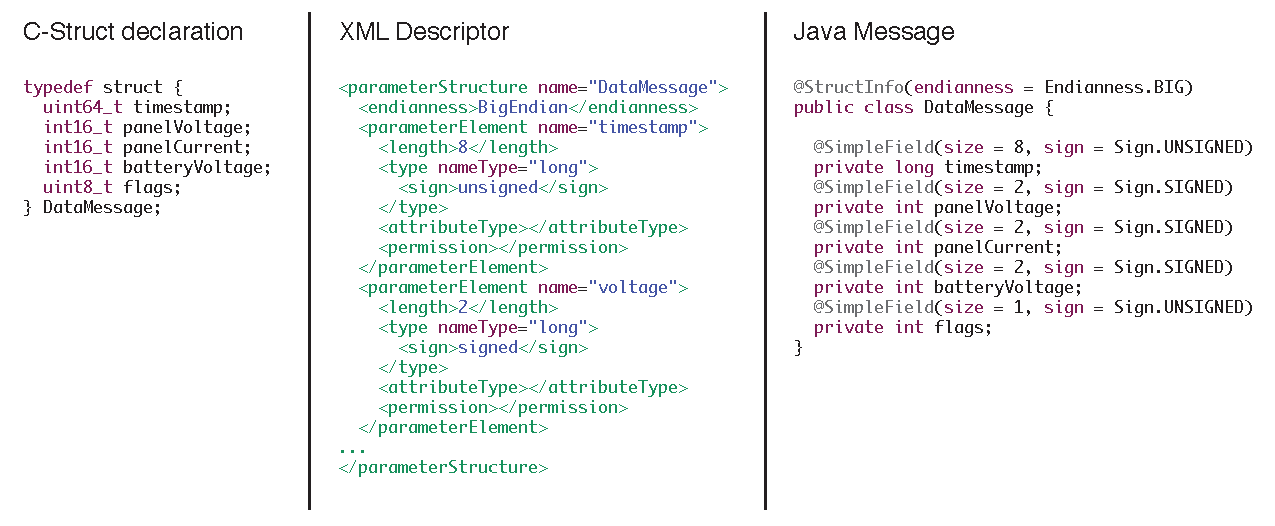
\includegraphics[width=\textwidth]{imgs/classic_descriptor.pdf}
\caption{Physical to logical attribute mapping in the Classic PerLa Middleware.
The annotations added to the Java Message allow the \texttt{Marshaller} and
\texttt{Unmarshaller} components to encode and decode the information exchanged 
with the remote device.}
\label{fig:classic_descriptor}
\end{figure}

All the information required to create the Java objects used during this
process, along with the corresponding attribute mappings and
\texttt{Marshaller}/\\texttt{Unmarshaller} directives, are extracted from the
Device Descriptor. Figure~\ref{fig:classic_descriptor} contains a typical
descriptor example, which highlights the correlations that exist between a
C-Struct declaration used in the sensing device, its corresponding Device
Descriptor, and the resulting Java class created by the \texttt{FPCFactory}.

Most of the concepts introduced in this brief description of the Classic PerLa
architecture will be subject of further discussion in
Chapter~\ref{cha:middleware_overview}, where they are going to be match
alongside their novel counterparts.

\section{The PerLa Query Language}
\label{sec:language}

The PerLa Query Language is a declarative, SQL-like language for interacting
with Pervasive Systems. A sensing network managed by PerLa is abstracted as a
large table in a streaming database, whose columns correspond to specific data
elements that can be retrieved from the devices connected to the Middleware.
This generalization allows final users to glean information out of a Pervasive
System without dealing with all the complications that stem from managing the
quirks of every single sensing node, as the intricate mesh of available data
sources is completely hidden by the database abstraction.

The PerLa Query Language is designed to be simple and easy to use. Its core
syntax is compact and reminiscent of other well-known database-oriented
languages as SQL. It provides a uniform interrogation mechanism that enables
the collection of data elements regardless of their origin. Information may be
sampled from a physical phenomena, read from the memory of an endpoint device
or estracted from a web service; whatever the source, the PerLa query pattern
is always the same.

PerLa queries allow the user to determine the exact behaviour of a data source
using a consice but powerful set of clauses. The reminder of this section will
provide an overview of the main syntactic and semantic features of the PerLa
Query Language, along with two examples excerpted from real-world use cases.

\subsection{The Data Management section}

Introduced by the \texttt{SELECT} clause, this section of the PerLa Query
Language should immediately result familiar to every person acquainted with the
SQL language. This clause achieves two purposes: first, it defines which data
elements (specifically, which data \texttt{Attributes}) are to be collected
from the Pervasive System; second, it indicates the operations and computations
that must be performed on the information extracted from the Pervasive System.

The need to manage a theoretically infinite stream of data elements coming from
the sensing network required the development of a custom syntax for aggregate
operations. Differently from standard SQL aggregates, which always operate on a
finite set of elements whose size is well-known at runtime, PerLa aggregates
must cope with an ever-flowing stream of records, and thus require users to
specify the scope of their intended computations. This is achieved through a
duration expression, an additional mandatory parameter that complements the
aggregation expression by limiting the number of records to be processed to a
limited amount. Duration expressions can be specified using two different
methods: a time-based syntax, that allows users to define the aggregation scope
in terms of time windows (\lstinline!SELECT AVG(TEMP, 10 SECONDS)!), and a
record-based syntax, that clearly indicates the number of records to be used
for the computation (\lstinline!SELECT AVG(TEMP, 30 SAMPLES)!).

\subsection{The Sampling section}

The Sampling section can be used to specify how and when the data elements
requested with the \texttt{SELECT} statement are to be extracted from the
network nodes. There are two different operating modes, both introduced by the
\texttt{SAMPLING} clause. \textit{Time-based} sampling can be used to collect
data at periodic intervals. The sampling frequency is specified by means of an
\texttt{IF-EVERY} syntax that enables users to specify different sampling
periods, along with the conditions for their activations. On the other hand,
the \textit{Event-based} sampling mode allows the acquisition of a data sample
each time the desired event is fired.

~\\
\begin{lstlisting}[caption={An example of time-based sampling, which shows how
the sampling frequency can be increased as the monitored phenomenon evolves.}]
SAMPLING
    IF temperature < 50 EVERY 10 MINUTES
    ELSE IF TEMPERATURE >= 50 EVERY 1 MINUTES
\end{lstlisting}

\subsection{The Conditional Execution section}

Introduced by the \texttt{EXECUTE IF} clause, this query section contains a
boolean expression that every sensing device must satisfy in order to be
considered as a candidate data source, and it's often employed when the user
requires its query to be executed on nodes with well-defined capabilities. This
section is not mandatory, and its omission implies that the PerLa query must be
executed on every device of the sensing network. An \texttt{EXECUTE IF}
statement can be optionally complemented by a \texttt{REFRESH} clause, which
specifies how often the execution condition is re-evaluated to update the list
of nodes involved in the evaluation of a query. 

\subsection{The Termination Condition section}

An optional clause that can be used to terminate the execution of a query, both
in terms of time (\lstinline!TERMINATE AFTER 1 DAY!) or number of selections
performed (\lstinline!TERMINATE AFTER 10 SELECTIONS!). This behaviour is useful
when perform a one-shot query, or when the monitoring period is known a priori.

\subsection{Query examples}

The following query initiates a temperature sampling operation on all
temperature sensors located in room number three. New data readings are
collected by the minute, as specified by the \texttt{SAMPLING} clause; however,
new output records are created every 5 minutes, as indicated in the
\texttt{EVERY} statement that guards the data management section. Finally, each
record produced by this query contains the maximum temperature value collected
in the previous 10 minutes of sampling.

\begin{lstlisting}
CREATE OUTPUT STREAM Table (Temperature FLOAT) AS:
EVERY 5 MINUTES
SELECT MAX(temp, 10 MINUTES)
SAMPLING
  EVERY 1 MINUTES
EXECUTE IF EXISTS(temp) AND EXISTS(room) AND room = 3
\end{lstlisting}


This second example illustrates how the PerLa Language can be used to collect
information in response to an event. First of all, this is a one-shot query, as
it terminates as soon as the first record is produced. The single output record
contains the number of times the RFID with identifier \texttt{0xDF445A} was
scanned in the last 10 minutes.

\begin{lstlisting}
CREATE OUTPUT STREAM Table (rfid STRING, counter INTEGER) AS:
EVERY 10 MINUTES
SELECT lastReaderId, COUNT(*, 10 MINUTES)
SAMPLING
  ON EVENT lastReaderChanged
EXECUTE IF ID=[0xDF445A]
TERMINATE AFTER 1 SELECTIONS
\end{lstlisting}


\section{Context management}


		\chapter{The New PerLa Middleware}
\label{cha:middleware_overview}

\section{Design goals}

Introduce the design goals of the new Middleware architecture

\section{Overview of the New Middleware Architecture}

As illustrated in the previous chapter, the PerLa Middleware is responsible for
managing the lifecycle of all devices connected to the PerLa framework, and for
providing a uniform API to interact with them. Its design revolves around the
Functionality Proxy Component (\texttt{FPC}), a self-contained proxy object
that embeds all the logic required to communicate with a single remote device.
The most prominent trait of the \texttt{FPC} is still its interface, an API
that allows PerLa users to interact with the sensing network through two
hardware-agnostic communication primitives, named get() and set(). Use of this
interface neither requires knowledge of the sensing network, nor of the device
that will ultimately perform the requested operation.

\subsection{The New FPC}

Differently from the Classic PerLa Middleware, the New \texttt{FPC} is formed
from the composition of various independent software units, each of which is
responsible for the management of a single aspect of the interaction with the
remote device (see figure~\ref{fig:fpc_overview}). This new modular design was
chosen to further promote reusability and foster future expandability through
composition of independent objects. The following remainder of this section
contains a summary of all modules that compose the new \texttt{FPC}
architecture.

\begin{figure}[h!]
\center
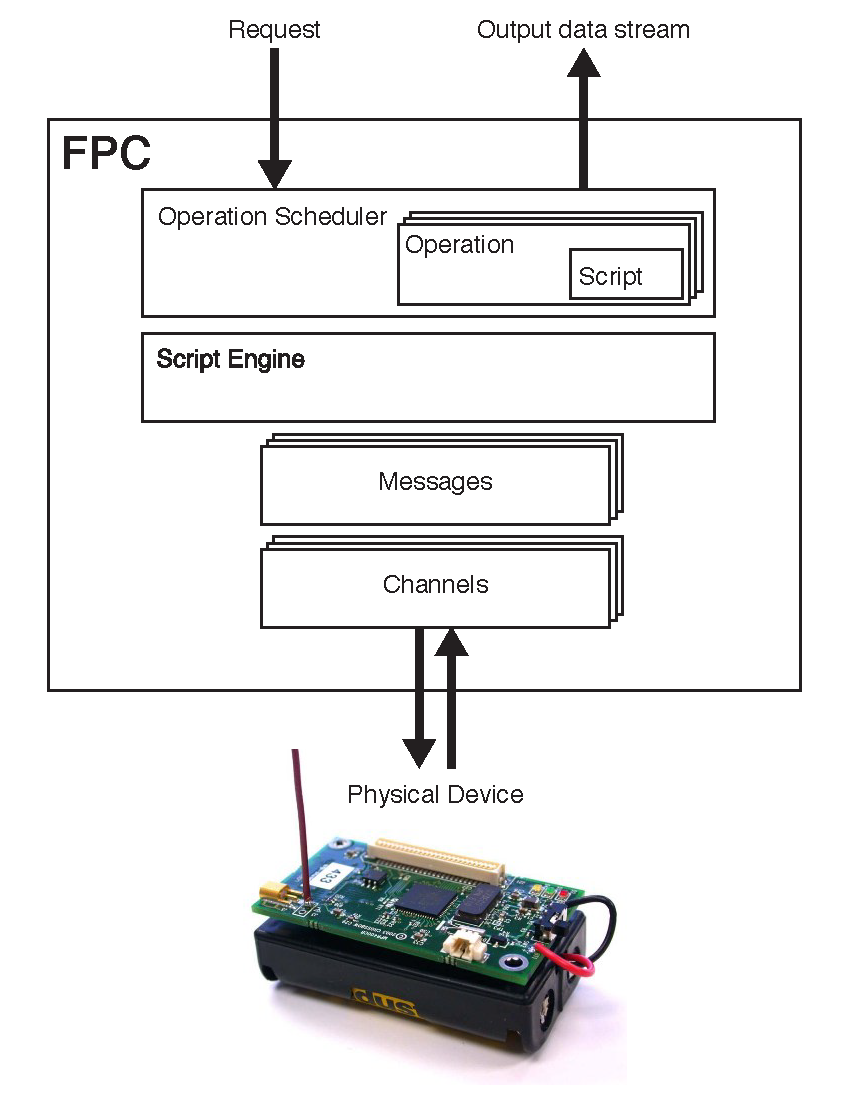
\includegraphics[width=0.6\textwidth]{imgs/fpc.pdf}
\caption{Internal structure of the new FPC component.}
\label{fig:fpc_overview}
\end{figure}

\subsubsection{Channel}

\texttt{Channel}s are software components capable of performing I/O operations.
They are commonly employed to manage the communication between PerLa and the
devices of a Pervasive System, and can be thought as a complete substitute of
the \texttt{Channel Manager}/\texttt{Virtual Channel} components. Unlike their
counterpart in the Classic architecture, \texttt{Channel}s are settled inside
the boundary of an \texttt{FPC}. This change of location has two important
consequences: first of all, it allows each \texttt{FPC} to make use of multiple
data transmission technologies for the exchange of information with the
controlled endpoint; second, it enhances the modularity of the entire PerLa
Middleware, as new communication systems and protocols can be introduced
without modifying any existing \texttt{Channel} implementations.

Every \texttt{Channel} is bundled with a collection of \texttt{IORequest}
objects, which are employed to initiate specific I/O tasks on the sensing
nodes. For example, the \texttt{HTTPChannel} --- a \texttt{Channel}
implementation of the HTTP protocol --- is bundled with four different
\texttt{IORequest}s, one for each of the principal HTTP methods (GET, POST, PUT
and DELETE).

\subsubsection{Mapper}

A software module for marshalling and unmarshalling data. \texttt{Mapper}s
allow the \texttt{FPC} to interpret byte streams received from a communication
\texttt{Channel}, and to serialize high-level data structures prior to
transmission. They perform as a more flexible alternative to the fixed
\texttt{Marshaller}-\texttt{Unmarshaller} components found in the Classic
\texttt{FPC} implementation.

Similarly to what already seen for the \texttt{Channel} component, every
\texttt{Mapper} implementation is responsible for managing a different
\texttt{Message} format, namely a different data encoding; therefore,
\texttt{FPC}s may employ different \texttt{Mapper} objects, each of which is
tasked with managing a well-defined data structure exchanged with the remote
device. This feature is in stark contrast with the Classic Middleware design,
which could only manage a single data format per device.

\subsubsection{Scripts and Operations}

\begin{itemize}

    \item \textbf{Script Engine:} An interpreter for executing PerLa
        \texttt{Scripts}, small programs written in a proprietary PerLa
        scripting language, which are used to dynamically bind high level data
        requests to native processing tasks performed on the remote device;

    \item \textbf{Operation Scheduler:} Schedules the execution of concurrent
        data collection operations on the remote device. The scheduler may
        simulate certain operations if the device connected to the FPC is not
        able to perform them natively (e.g., periodic sampling may be simulated
        by polling the remote device at regular intervals).

\end{itemize}

\begin{figure}[h!]
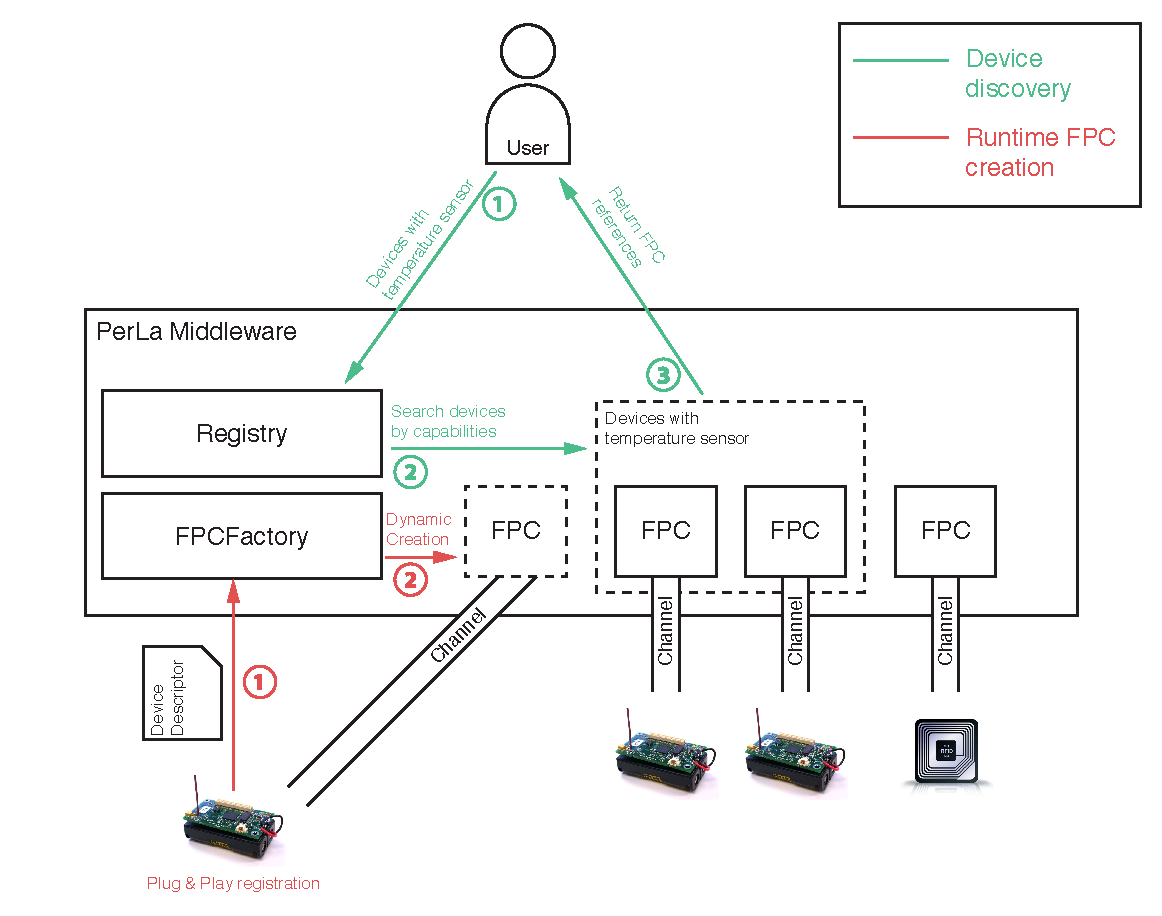
\includegraphics[width=\textwidth]{imgs/middleware_overview.pdf}
\caption{The PerLa Middleware architecture}
\end{figure}

New \texttt{FPC} objects are instantiated at runtime by the
\texttt{FPCFactory}. The starting point for the creation of an \texttt{FPC} is
the Device Descriptor, an XML document which contains a machine parseable
description of a single sensing device. Device Descriptors are organised in
different sections, each of which defines the configuration of one of the
aforementioned \texttt{FPC} modules. The \texttt{FPCFactory} can receive new
Device Descriptors directly from the node being connected (Plug\&Play
behaviour), or from another entity that acts on behalf of it (off-band
behaviour). The latter approach allows devices which are not capable of
autonomously transmit their Device Descriptor to be registered on the PerLa
Middleware.

A reference to each \texttt{FPC} is stored in the \texttt{Registry}, a
Middleware component that is responsible for maintaining a complete index of
all devices accessible through the PerLa framework. Thanks to the
\texttt{Registry}, PerLa user can discover sensing nodes through
capability-based queries, and retrieve the \texttt{FPC} objects that can be
used to interact with them.


\section{Differences with the Classic Middleware}

\subsection{Asynchronous interaction paradigm}
\label{sec:newmiddleware.async}

One of the major differences between the New and Classic Middleware
architectures lies in the technique employed to interconnect internal modules
of the PerLa software infrastructure. The New Middleware introduces a fully
asynchronous interaction paradigm based on non-blocking method invocations and
event-driven programming techniques, which deviates profoundly from the
mechanism previously promoted in the Classic design.

\begin{figure}[h!]
    \center
    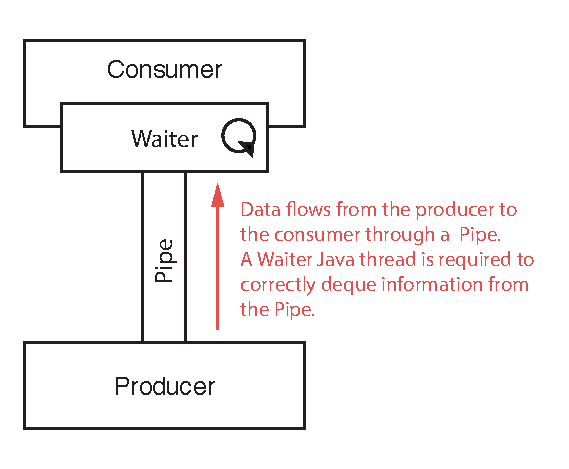
\includegraphics[width=0.5\textwidth]{imgs/pipe_waiter.pdf}
    \caption{A typical \texttt{Pipe}-\texttt{Waiter} connection in the Classic
        PerLa Middleware}
\end{figure}

Within the previous Middleware architecture, a connection between two different
modules was achieved by means of a decoupling element dubbed \texttt{Pipe}, a
one-way message queue designed to shuttle data elements from a software
component to its intended receiver. This system proved to be crucial in the
first development stages of PerLa, as its generic interface allowed the early
designers to experiment with several competing architectures and component
combinations. However, its flexibility came at a cost, both in terms of
performances and API readability. First of all, each \texttt{Pipe} allocated an
initial memory cache of 10 elements. Moreover, the receiving end of a
\texttt{Pipe}, namely the \texttt{Waiter}, was required to instantiate a Java
thread dedicated solely to the reception of data messages. The widespread use
of the \texttt{Pipe}-\texttt{Waiter} paradigm thus led to the proliferation of
threads and to an overuse of memory, which negatively impacted the overall
system efficiency. In addition, the loosely coupled interaction paradigm
promoted by the Classic Middleware resulted in a weak API that lacked intent
and semantic clarity.

The asynchronous, event-driven architecture implemented in the New Middleware
overcomes all aforementioned drawbacks, and improves system performances in
terms of both throughput and scalability. Differently from the deprecated
\texttt{Pipe}-driven system, this new design fosters a direct exchange of
information between data producers and data consumers; information is no more
delivered using a mandatory middleman (i.e., the \texttt{Pipe}), but is
explicitly handed over to the intended recipients. This interaction paradigm is
based on the \textit{Hollywood Principle}, a software design methodology whose
tenets are summarized by the motto ``\textit{don't call us, we call you}'',
that encourages the development of highly-cohesive, low-coupling APIs, 

\begin{figure}[h!]
\center
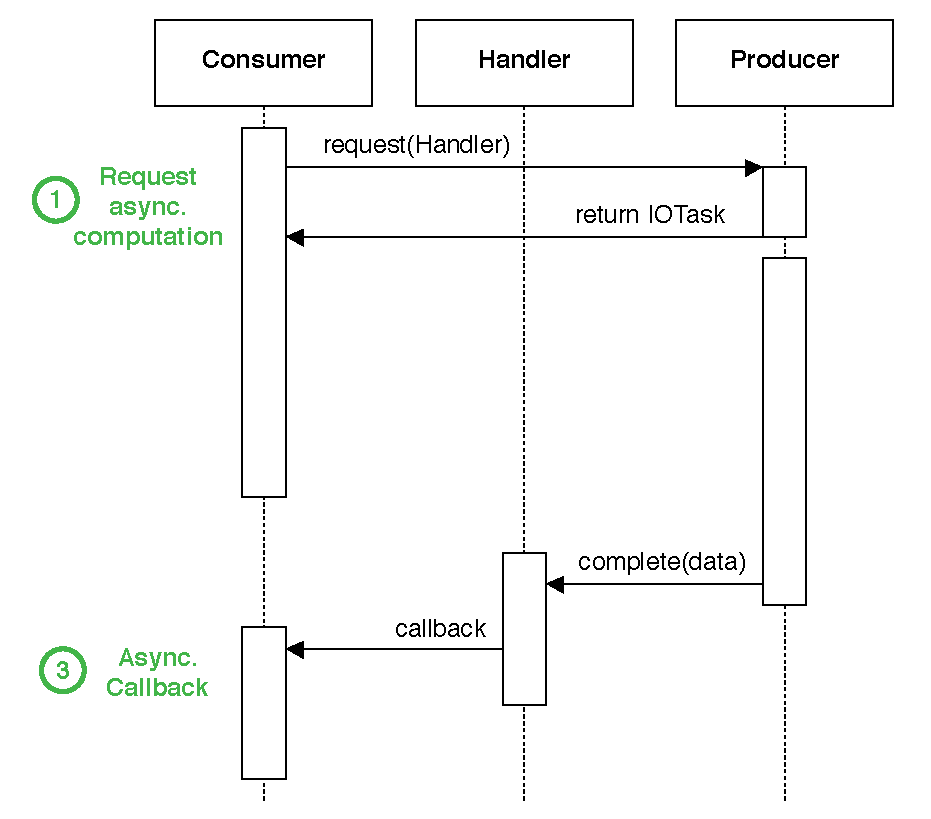
\includegraphics[width=0.8\textwidth]{imgs/async_paradigm.pdf}
\caption{Sequence diagram of an asynchronous method call. Note that the
consumer and the producer continue their execution in parallel.}
\label{fig:async_paradigm}
\end{figure}

Every asynchronous method call in the New PerLa Middleware is identified by the
following characteristics:

\begin{itemize}

    \item \textbf{Does not block:} Calls to an asynchronous method never block;
        control of the execution flow is immediately returned to the caller,
        and the requested computation is executed asynchronously. This
        characteristics reduces the number of Java threads that the caller
        module needs to instantiate;

    \item \textbf{Returns a Task object:} Asynchronous method calls do not
        return the immediate result of a computation. Instead, they return a
        \texttt{Task}, i.e., an object that can be employed to stop the ongoing
        operation or to query its current state of progress;

    \item \textbf{Defers the delivery of results:} The effective result of an
        asynchronous method is notified through a \texttt{Handler} function,
        which is invoked as soon as the computation terminates.

\end{itemize}

For an in-depth description of the actual asynchronous APIs implemented within
the PerLa Middleware, refer to chapter~\ref{cha:components}.


\subsection{FPCFactory Plugin System}
\label{sec:newmiddleware.factory}

The new \texttt{FPCFactory} is a modular software entity composed of multiple
factory components dedicated to the creation of a specific \texttt{FPC} module.
Its design is a significant departure from the original monolithic factory
structure, and allows final users to easily expand the base capabilities of the
PerLa Middleware without modifying its original source code. This modular
architecture, formally called \texttt{FPCFactory} Plugin System, is a direct
implementation of the \textit{Open/Close} principle: the \texttt{FPCFactory}
is open for extension, as its functionalities can be expanded by adding new
plugins, but closed for modification, since the addition of a new sub-factory
does not require any change to the Middleware's source code.

At the current state of implementation, the PerLa Middleware supports three
different \texttt{FPCFactory} plugin types, viz. \texttt{ChannelFactories},
\texttt{IORequestFactories} and \texttt{MapperFactories}, which are responsible
for the creation of new \texttt{Channels}, \texttt{IORequests} and
\texttt{Mappers} respectively. All implementations of a single plugin type are
tasked with creating the same class of \texttt{FPC} modules; for example, the
\texttt{HTTPChannelFactory} and the \texttt{TinyOSChannelFactory} both create
\texttt{Channel} objects, but the first are used to connect with RESTful web
APIs, whereas the second are interfaces to TinyOS networks.

The introduction of a new modular \texttt{FPCFactory} Plugin System resulted in
a complete redesign of the Device Descriptor itself, which changed its layout
to accomodate a modular structure that closely follows the new
\texttt{FPCFactory} architecture. The new Device Descriptor is composed of the
following elements:

\begin{itemize}

    \item \textbf{Preamble:} Represented by the root \lstinline!<device>! tag,
        this section contains a textual description of the endpoint, and a list
        of XML namespaces. As shown later, namespaces are employed to select
        the various Device Descriptor features and \texttt{FPCFactory} plugins
        required for the creation of an \texttt{FPC} object;

    \item \textbf{Attribute declarations:} A list of all the device
        \texttt{Attributes} exposed by the device. It must be enclosed in an
        \lstinline!<attribute>! XML tag;

    \item \textbf{Channel declarations:} This section contains the
        configuration options of all \texttt{Channel} objects required to
        communicate with the remote device. Its contents are parsed and
        interpreted by the \texttt{ChannelFactory} plugins, whose structure is
        discussed in section~\ref{sec:channel};

    \item \textbf{Message declarations:} A section reserved for the declaration
        of all data structures required to exchange information with a node of
        the network. Its contents are directly interpreted by the
        \texttt{MapperFactory} plugins to create new \texttt{Message}
        mappers, as described in section~\ref{sec:components.mapper};

    \item \textbf{Request declarations:} This part of the Device Descriptor is
        reserved for the declaration of all \texttt{IORequest} objects needed
        to communicate with a remote device. The elements hereby contained are
        processed by the \texttt{IORequestFactory} plugins, as per instructions
        given in section~\ref{sec:channel};

    \item \textbf{Operation declarations:} As shown in
        section~\ref{sec:components.fpc}, this final portion of the Device
        Descriptor contains all PerLa \texttt{Scripts} employed to control the
        remote device.

\end{itemize}

~\\
\lstset{language=XML}
\begin{lstlisting}[caption={The skeleton of the new XML Device Descriptor.}]
<?xml version="1.0" encoding="UTF-8"?>
<device type="test" xmlns="http://perla.dei.org/device">
  <attribute>
    <!-- Attribute declarations -->
  </attribute>
  <channel>
    <!-- Channel declarations -->
  </channel>
  <message>
    <!-- Message declarations -->
  </message>
  <request>
    <!-- IORequest declarations -->
  </request>
  <operation>
    <!-- Operation and Scripts -->
  </operation>
</device>
\end{lstlisting}

As briefly explained in previous paragraphs, XML namespaces constitute a
fundamental element of the \texttt{FPCFactory} Plugin System, since they are
used to select which factory component must be employed for the creation of a
specific \texttt{FPC} module. A practical example of this concept is available
in figure~\ref{fig:dd_namespace}: this Device Descriptor excerpt specifies two
plugin namespaces, one for a \texttt{HTTPChannel}
(\texttt{http://perla.dei.org/fpc/channel/http}), and the other for a
\texttt{JSONMapper} (\texttt{http://perla.dei.org/fpc/message/json}); these two
values, once processed by the texttt{FPCFactory}, are used for selecting the
specific plugin that will be used for constructing the corresponding
\texttt{FPC} components. It is important to note that the
\texttt{http://perla.dei.org/device} and
\texttt{http://perla.dei.org/device/instructions} namespaces are mandatory, as
they respectively define the Device Descriptor base elements and all available
\texttt{Script} instructions.

\begin{figure}[h!]
\center
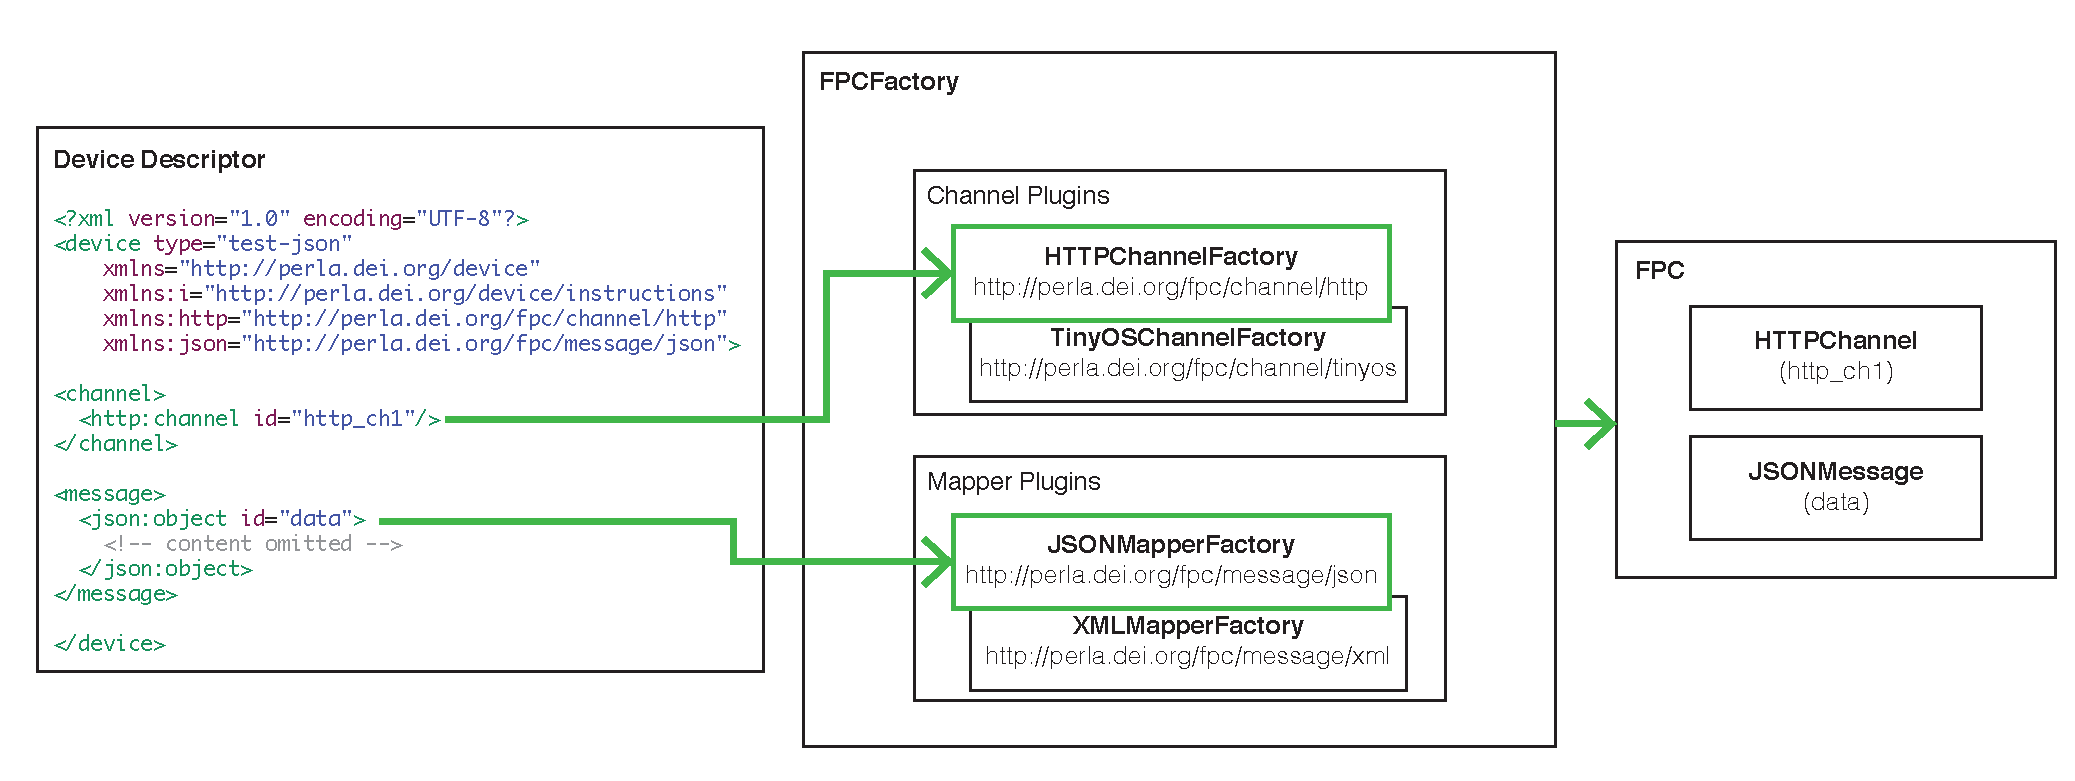
\includegraphics[width=\textwidth]{imgs/dd_namespace.pdf}
\caption{Namespace-guided FPC creation.}
\label{fig:dd_namespace}
\end{figure}

Every \texttt{FPCFactory} plugin is also responsible for defining the
particular XML syntax to be used in its Device Descriptor section. This feature
endows plugin authors with the opportunity to specify a custom set of options
to be used for the creation of their \texttt{FPC} modules. The possibility of
using a custom syntax is key to the new \texttt{FPCFactory} Plugin System,
since different types of plugins may require totally different configuration
values in order to be used or even initialized (e.g., communicating over a HTTP
\texttt{Channel} is considerably different than sending data on a low-power
mesh network).

\subsection{PerLa Scripting system}




		\chapter{In-depth component description}
\label{cha:components}

\section{Communicating with Channels}
\label{sec:channel}

\texttt{Channel} is an interface for performing I/O operations. It represents
the principal abstraction used by the middleware to communicate with hardware
devices and external software services.

\lstset{language=Java}
\begin{lstlisting}[float,caption=The Channel interface,label={lst:channel}]
public interface Channel {

	public String getId();
	
	public IOTask submit(IORequest request, IOHandler handler)
			throws ChannelException;
	
	public void setAsyncIOHandler(IOHandler handler)
			throws IllegalStateException;
			
	public boolean isClosed();
	
	public void close();
			
}
\end{lstlisting}

The \texttt{Channel} interface is not tied to any specific technology or
communication stack; as a result of this design choice, a wide variety of data
management tasks, including but not limited to, networking, file handling, and
automatic data generation can be implemented as \texttt{Channel}s.

The current Middleware architecture encourages the creation of several highly
specialized \texttt{Channel}s, which are usually developed around third-party
communication libraries. \texttt{HTTPChannel}, a \texttt{Channel} providing
support for HTTP communications, is an excellent example of the advantages of
this design strategy. Implemented as a simple wrapper around Apache's HTTP
Components toolkit, its development only required a basic understanding of the
HTTP protocol; yet \texttt{HTTPChannel} is a fully compliant HTTP/1.1 client.

Upon instantiation, \texttt{Channel}s are open and ready to be used. They may
be optionally closed to relinquish unused resources by invoking the
\texttt{close()} method. Once closed, a \texttt{Channel} cannot be re-opened,
and every subsequent attempt to perform an I/O operation will fail causing a
\texttt{ChannelException} to be thrown. The current state of a \texttt{Channel}
can be probed through its \texttt{isClosed()} method.

Bytes sent or received with a \texttt{Channel} are encapsulated in a
\texttt{Payload} object. As shown in listing~\ref{lst:payload}, the
\texttt{Payload} interface allows all Middleware components to handle different
data types with a common set of methods, regardless of their individual
encoding.  \texttt{Payload}s will be the subject of further discussion in
section~\ref{sec:components.mapper}

\lstset{language=Java}
\begin{lstlisting}[float,caption=The Payload interface,label={lst:payload}]
public interface Payload {

	public Charset getCharset();

	public InputStream asInputStream();

	public ByteBuffer asByteBuffer();

	public String asString();

}
\end{lstlisting}

All user-initiated I/O operations begin with an invocation of the
\texttt{Channel.submit()} method. As can be seen in listing~\ref{lst:channel},
\texttt{submit()} is a direct implementation of the asynchronous interaction
paradigm introduced in section~\ref{sec:newmiddleware.async}. The emphasis on
asynchronous execution is underscored by the absence of blocking operations in
the \texttt{Channel} interface. This aspect is of paramount importance for the
entire Middleware design, as implementing a truly asynchronous system would
prove impossible if such feature were not provided by its core data access
layer.


\subsection{Instantiating new Channels}

\texttt{Channel}s are created by means of the \texttt{ChannelFactory}
interface, a reification of the Factory design pattern that allows polymorphic
instantiation of new object classes.

By using a Factory instantiation model, the choice of a particular
\texttt{Channel} implementation can be postponed from compile time to run time.
This technique allows the Middleware to dynamically adapt in response to
environment changes, and to support extension through the addition of new
user-defined \texttt{Channel}s. For further information regarding the Factory
pattern and its other uses inside the PerLa Middleware, refer to
section~\ref{sec:newmiddleware.factory}.

All the information required to create a new \texttt{Channel} is stored inside
a \texttt{ChannelDescriptor}. As shown in listing~\ref{lst:channelFactory},
this configuration object is the only parameter required to correctly invoke
the \texttt{createChannel()} method.

\lstset{language=Java}
\begin{lstlisting}[float,caption=The ChannelFactory
interface,label={lst:channelFactory}]
public interface ChannelFactory {

	public Class<? extends ChannelDescriptor>
			acceptedChannelDescriptorClass();

	public Channel createChannel(ChannelDescriptor descriptor)
			throws InvalidDeviceDescriptorException;

}
\end{lstlisting}

\begin{figure}[h!]
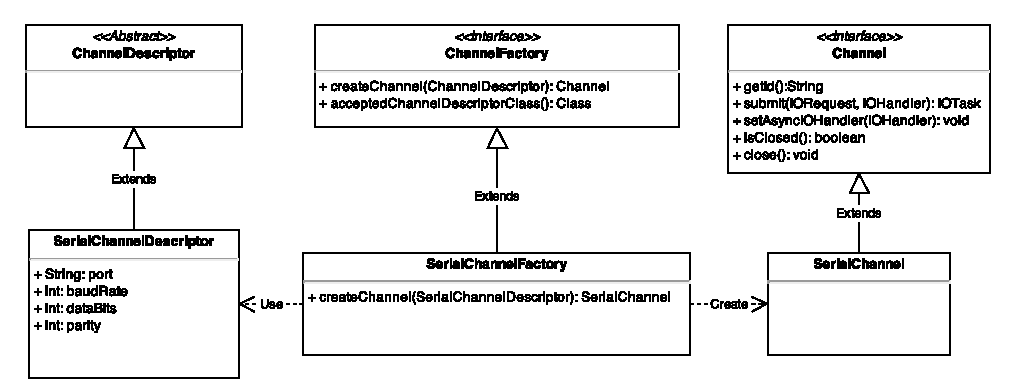
\includegraphics[width=\textwidth]{imgs/channel_factory.pdf}
\caption{Class diagram of the Channel layer}
\end{figure}

Each \texttt{ChannelFactory} is tied to a specific communication technology;
therefore, it can only accept a single class of \texttt{ChannelDescriptor}
objects. For example, the \texttt{HTTPChannelFactory} parses
\texttt{HTTPChannelDescriptor}s and creates \texttt{HTTPChannel}s, whereas an
hypothetical \texttt{SerialChannelFactory} would consume
\texttt{SerialChannelDescriptor}s to create \texttt{SerialChannel}s. Failure to
provide a suitable \texttt{ChannelDescriptor} object will cause the
\texttt{createChannel()} method to throw an
\texttt{InvalidDeviceDescriptorException}.

The \texttt{acceptedChannelDescriptorClass()} method can be used to dynamically
discover which \texttt{ChannelDescriptor} type is supported by a specific
\texttt{ChannelFactory}. This method is the fulcrum of the \texttt{Channel}
Plugin System, as it allows the Middleware to invoke the most appropriate
\texttt{ChannelFactory} using only information available at runtime.

\begin{figure}[!hbt]
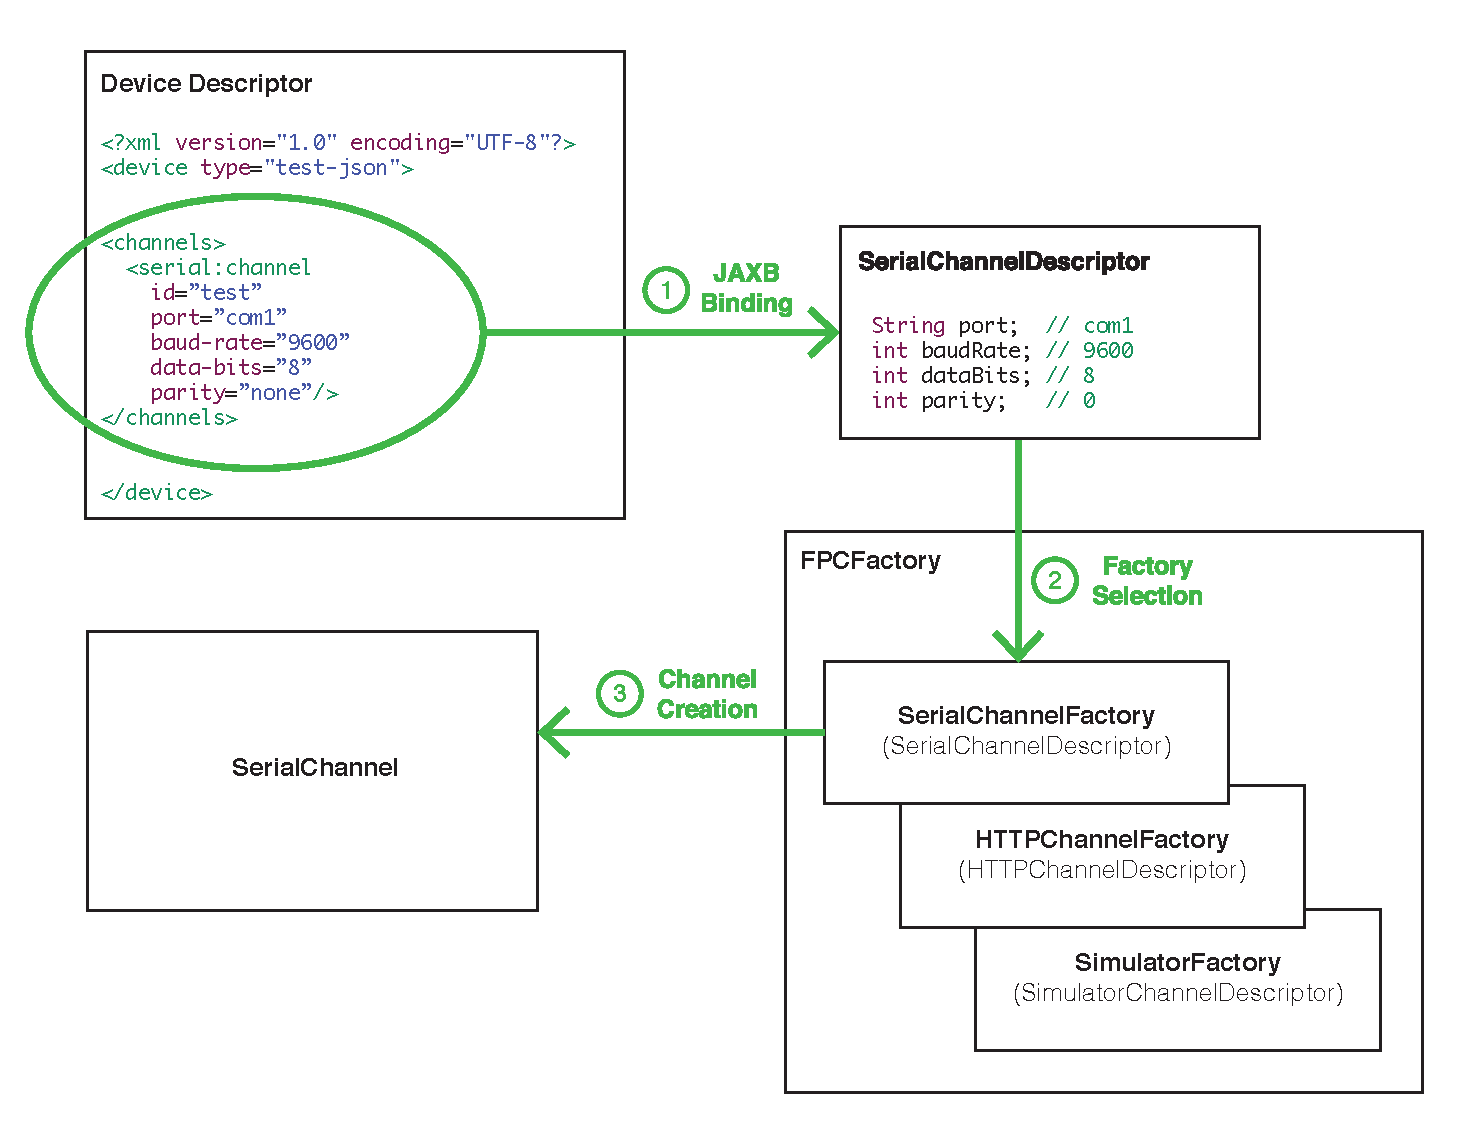
\includegraphics[width=\textwidth]{imgs/channel_creation_process.pdf}
\caption{The Channel creation process}
\label{fig:channel.creation}
{
\begin{figurenote}
This figure illustrates the \texttt{Channel} creation process executed by the
Middleware upon reception of a new Device Descriptor.
\begin{enumerate}
  \itemsep0em
  \item JAXB binds the XML Device Descriptor to an apropriate
\texttt{ChannelDescriptor} object using namespace information \item A suitable
\texttt{ChannelFactory} is selected at runtime using the
\texttt{acceptedChannelDescriptorClass()} method
  \item The information contained in the \texttt{SerialChannelDescriptor} is
used to create a new \texttt{SerialChannel}
\end{enumerate}
\end{figurenote}
}
\end{figure}

\texttt{ChannelDescriptor} objects are automatically created by the
Middleware using the information contained in the Device Descriptor XML files.
This binding process is performed by the JAXB library, which is also
responsible for instantiating the correct \texttt{ChannelDescriptor} class
using XML Namespace information. Figure~\ref{fig:channel.creation} illustrates
this technique, and ties it together with the other operations described in
this section.

It is important to note that a single JVM instance running the PerLa Middleware
may host several \texttt{Channel} objects of the same type, at the same time.
Several devices can use the same communication technology, and the
\texttt{ChannelFactory} may determine that it's best to create an individual
\texttt{Channel} for each one of them. This behaviour is fostered by the new
\texttt{ChannelFactory} architecture, and is considered idiomatic design;
hence, it would not be uncommon to implement the hypothetical
\texttt{SerialChannelFactory} introduced in the previous paragraphs so that
every serial port is handled by a different \texttt{SerialChannel} instance.


\subsection{IORequest management}

\texttt{IORequest} is the base object interface employed to interact with a
sensing node connected to the Middleware. It contains two types of information:
the payload to be transferred, and \texttt{Channel}-dependent data needed for a
correct communication with the endpoint device.

\lstset{language=Java}
\begin{lstlisting}[float,floatplacement=!hbt,caption=The IORequest
interface,label={lst:iorequest}]
public interface IORequest {

	public String getId();

	public void setParameter(String name, Payload payload);
	
}
\end{lstlisting}

Every \texttt{Channel} imlementation is bundled with its own custom
\texttt{IORequest} class. Following up on previous examples, the
\texttt{HTTPChannel} package contains a \texttt{HTTPIORequest} object, whereas
the fictitious \texttt{SerialChannel} would be supplied with a
\texttt{SerialIORequest} class of request objects. This additional level of
indirection is necessary since different communication technologies require
different settings to establish end-to-end connectivity; therefore, a universal
\texttt{IORequest} object would soon prove to be a limiting factor for the
extension of the Middleware.

As shown in listing~\ref{lst:iorequest}, payload data can be set in an
\texttt{IORequest} by means of the \texttt{setParameter()} method.
\texttt{Payload}s are addressed by name, and a single \texttt{IORequest}
implementation may support several at once. The exact set of \texttt{Payload}
parameters accepted by an \texttt{IORequest} class depends on the design of its
matching \texttt{Channel}; for example, the \texttt{HTTPChannel}
implementation supports three: an `entity' payload (request body), a `query'
payload (an URL-encoded string), and a `path' payload (a path component used to
identify a single resource accessible from the base URL).

\texttt{IORequest}s are disposable objects; they are created, submitted to a
\texttt{Channel}, and garbage collected once the communication is over.
Creation is performed by means of a factory interface dubbed
\texttt{IORequestBuilder}, which allows the Middleware to build new copies of
an \texttt{IORequest} from a fixed template. It is important to note that
request objects built using this technique do not contain \texttt{Payload}
parameters; these are to be added manually before subbmitting the
\texttt{IORequest} to a \texttt{Channel}.

Besides \texttt{IORequest} creation, the \texttt{IORequestBuilder} interface
can be used to dynamically discover which \texttt{Payload} parameters are
supported by an \texttt{IORequest}. This functionality, exposed through the
\texttt{getParameterList()} method, is a crucial component of the Middleware
Plugin System, as it allows \textit{Script} instructions to determine whether
an \texttt{IORequest} was populated with all the necessary \texttt{Payload}
parameters or not. This concept will be the subject of further analysis in
section~\ref{sec:components.script}.

A single device connected to the PerLa Middleware is generally managed using
several \texttt{IORequestBuilder}s, any one of which is responsible for
creating a request object suitable to control a single aspect of
the interaction with the endpoint. The main advantage brought by this
templating mechanism is that \texttt{Channel}-related configuration settings
are only specified once, hence the same \texttt{IORequest} structure can be
reused multiple times to transport different payload information.

~\\
\lstset{language=Java}
\begin{lstlisting}[floatplacement=!hbt,caption=The IORequestBuilder
interface,label={lst:iorequestbuilder}]
public interface IORequestBuilder {

	public String getRequestId();

	public IORequest create();

	public abstract List<IORequestParameter> getParameterList();

	public static class IORequestParameter {

		public String getName() {
			return name;
		}

		public boolean isMandatory() {
			return mandatory;
		}

	}
}
\end{lstlisting}

REST APIs are an excellent use case to demonstrate the aforementioned concept,
as every operation on a RESTful resource can be easily abstracted using an
appropriately configured request builder. By using
\texttt{HTTPIORequestBuilder} objects, HTTP protocol information (base URL,
method, header, \ldots) are specified one single time only for
every REST endpoint. Once this step is done, the API can be invoked just by
building new \texttt{IORequest}s and submitting them to a \texttt{HTTPChannel}.

\begin{figure}[!hbt]
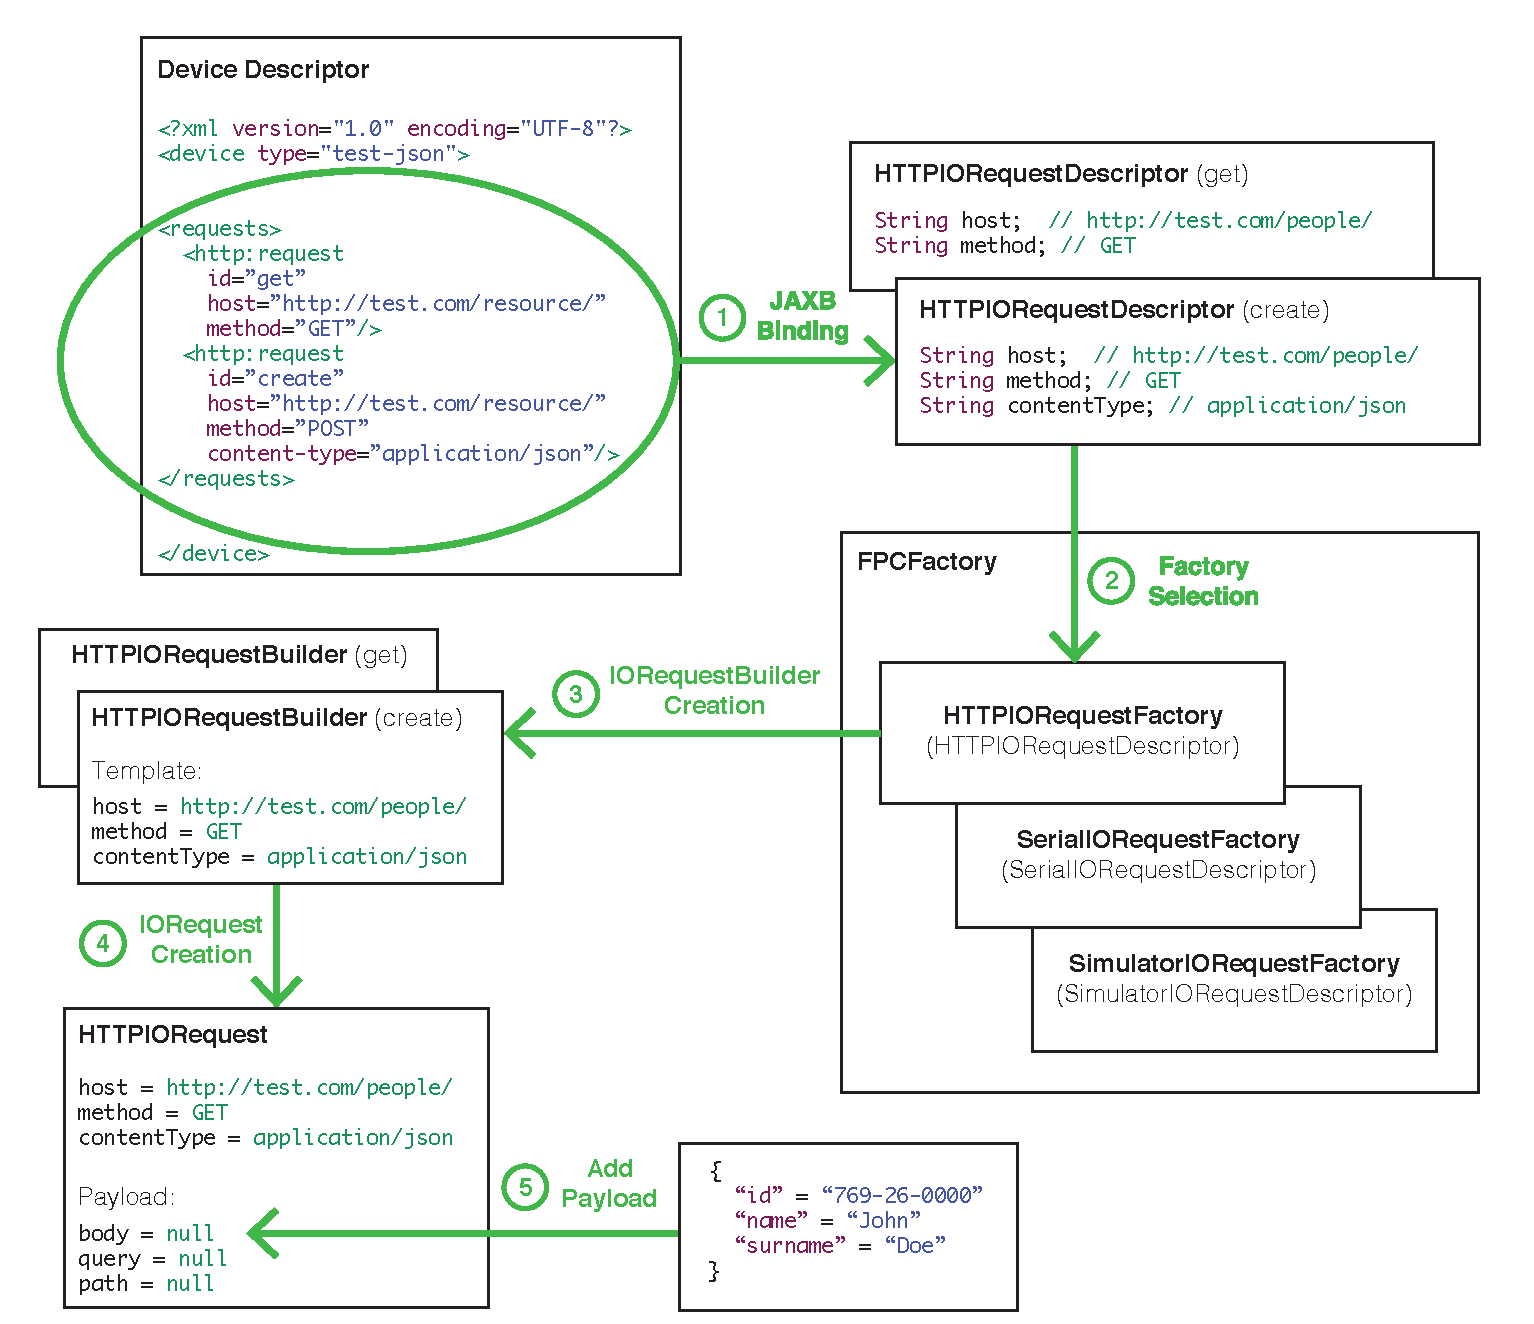
\includegraphics[width=\textwidth]{imgs/iorequest_creation_process.pdf}
\caption{The IORequest creation process}
\label{fig:iorequest.creation}
{
\begin{figurenote}
This figure illustrates the autonomous creation of \texttt{IORequest} objects.
Steps 1 to 3 are performed only once after receiving the Device Descriptor,
whereas steps 4 and 5 are repeated every time the REST API is to be invoked.
\begin{enumerate}
  \itemsep0em
  \item JAXB binds the XML Device Descriptor to an apropriate
\texttt{IORequestDescriptor} object using namespace information \item A
suitable \texttt{IORequestBuilderFactory} is selected at runtime using the
\texttt{acceptedIORequestDescriptorClass()} method
  \item The information contained in the \texttt{IORequestDescriptor} is used
to create a new \texttt{IORequestBuilder} \item The \texttt{IORequestBuilder}
is used to create new \texttt{IORequest} copies using the internal template
  \item The newly created \texttt{IORequest} objects can be populated with
\texttt{Payload} parameters as needed \end{enumerate}
\end{figurenote}
}
\end{figure}

\texttt{IORequestBuilder}s are created by means of an
\texttt{IORequestBuilderFactory}, an object that implements the now familiar
Factory design pattern. Creation proceeds as follows: the request template is
loaded from an XML Device Descriptor, bound to an appropriate
\texttt{IORequestDescriptor}, and processed by the
\texttt{IORequestBuilderFactory} to create the corresponding
\texttt{IORequestBuilder}. Similarly to what already seen in the previous
section, every \texttt{IORequestBuilderFactory} implements an
\texttt{acceptedIORequestDescriptorClass()} method, which can be used to
dynamically determine if a factory object can parse a specific type of
\texttt{IORequestDescriptor}. It should come as no surprise that every
\texttt{IORequestBuilder} class is provided with complementary
\texttt{IORequestBuilderFactory} and \texttt{IORequestDescriptor}
implementations.

\begin{figure}[!hbt]
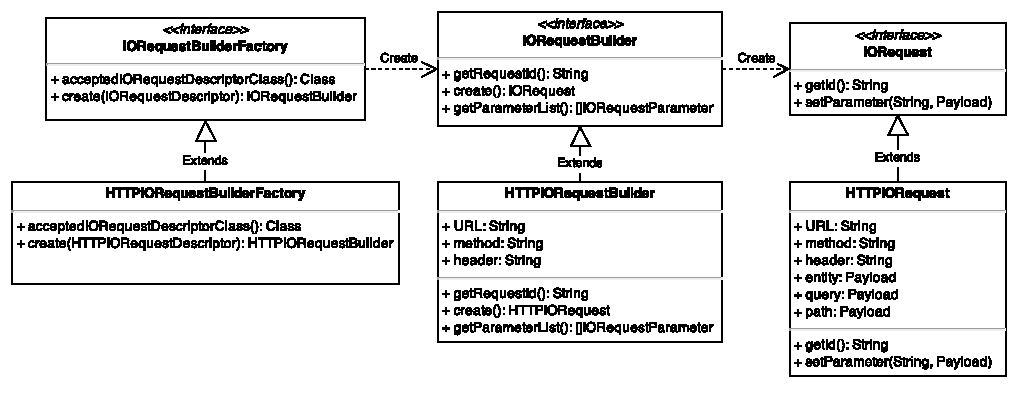
\includegraphics[width=\textwidth]{imgs/iorequest.pdf}
\caption{The extended IORequest class diagram. For additional information about
the IORequestParameter object consult listing 1.5.} \label{fig:iorequest.class}
\end{figure}


\subsection{Handling asynchronous I/O operations}

As mentioned in previous sections, communication with a device connected to the
PerLa Middleware is achieved by means of the \texttt{Channel.submit()} method.
Invocations of \texttt{submit()} are non-blocking; control flow is immediately
returned to the caller, thus allowing other computations to be performed while
the requested I/O operation is being processed.

As can be seen in listing~\ref{lst:channel}, \texttt{submit()} requires two
parameters: an \texttt{IORequest} and an \texttt{IOHandler} callback object.
The former specifies which I/O operation is to be performed, while the latter
allows the caller to be asynchronously notified of its completion.

The \texttt{IOHandler} interface is composed of two methods, namely
\texttt{complete()} and \texttt{error()}, which are invoked when processing of
an I/O operation comes to an end. It is important to note that both these
methods always carry context information in the form of an \texttt{IORequest},
which is guaranteed to be the same exact object used for starting the I/O
operation whose completion is being notified. For this reason,
\texttt{IOHandler} can be considered the nexus of the asynchronous invocation
model, as it connects \texttt{IORequest} objects with the outcome of the
corresponding I/O operation performed by the \texttt{Channel}.

\lstset{language=Java}
\begin{lstlisting}[float,floatplacement=H,caption=The IOHandler
interface,label={lst:iohandler}]
public interface IOHandler {
	public void complete(IORequest request, Optional<Payload> result);
	
	public void error(IORequest request, Throwable cause);
}
\end{lstlisting}

\lstset{language=Java}
\begin{lstlisting}[float,floatplacement=!hbt,caption=The IOTask
interface,label={lst:iotask}]
public interface IOTask {
	public void cancel();
	
	public IORequest getRequest();
	
	public boolean isCancelled();
	
	public boolean isDone();
}
\end{lstlisting}

Semantically, an invocation of the \texttt{complete()} method is always
associated with the successful termination of an I/O operation. As shown in
listing~\ref{lst:iohandler}, this method includes an optional \texttt{Payload}
object, that contains all data received from the endpoint device. A call to
\texttt{complete()} with an empty \texttt{Payload} indicates that the I/O
operation was completed without errors, but no data was received. Conversely,
an invocation of the \texttt{error()} method indicates that the I/O operation
was aborted before completion. In this case the cause of failure is always
notified through the \texttt{cause} parameter.

From the point of view the Java memory model, the \texttt{Channel.submit()}
creates a happens-before relationship with \texttt{IOHandler.complete()} and
\texttt{IOHandler.error()}, viz. any side effect generated by the code that led
to the \texttt{submit()} invocation is guaranteed to be visible in the
\texttt{complete()} and \texttt{error()} callback methods.

Asynchrous execution does not imply loss of control; ongoing I/O operations can
be monitored or cancelled by means of the \texttt{IOTask} object acquired upon
submitting an \texttt{IORequest}. Listing~\ref{lst:iotask} shows all methods of
the \texttt{IOTask} interface; method names are self explanatory, and the
reader should be able to deduce their purpose just by analyzing their 
signature. The only nuance worth mentioning is that
\texttt{isCancelled()} always implies \texttt{isDone()} (i.e., all cancelled
I/O operations are also complete), while the opposite does not hold (i.e., not
all complete I/O operations were cancelled).

\begin{figure}[!hbt]
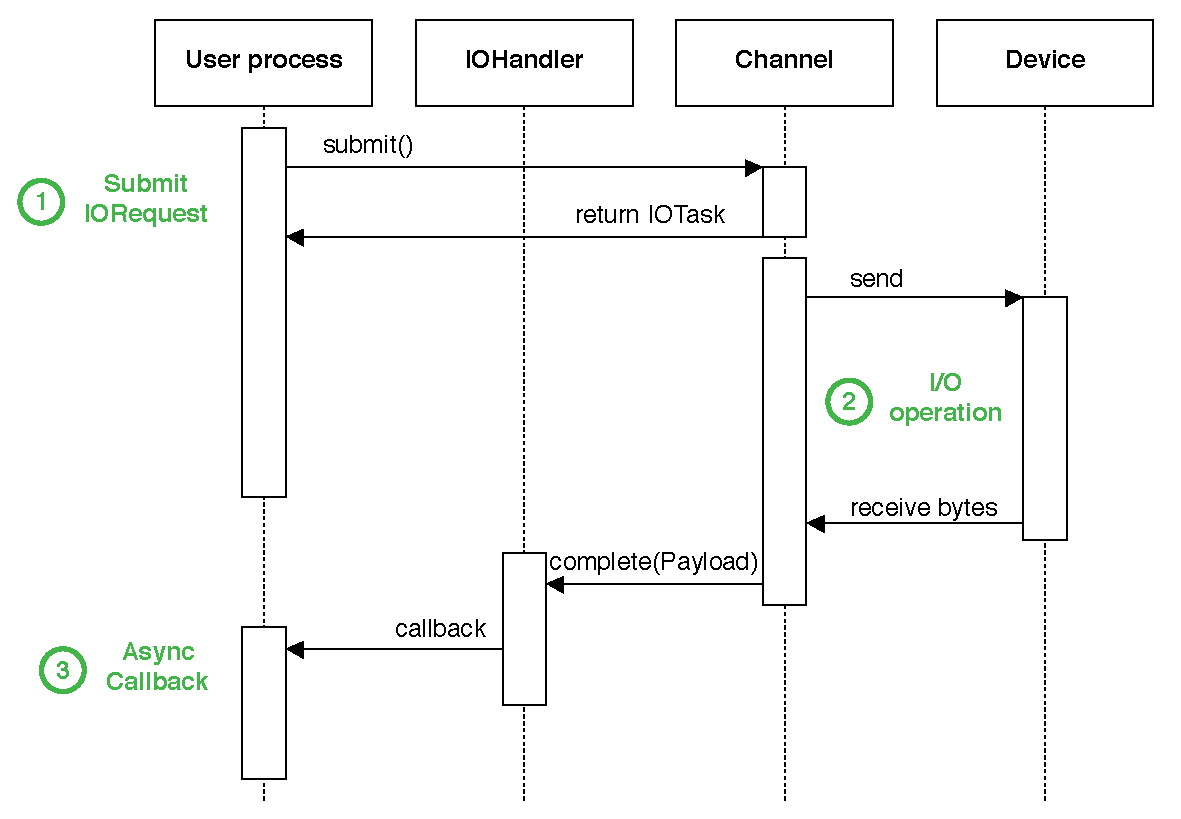
\includegraphics[width=\textwidth]{imgs/async_channel_sequence.pdf}
\caption{Sequence diagram of an asynchronous I/O operation. Note that the user
process and the I/O operation are executed in parallel.}
\label{fig:channel.async}
\end{figure}

The \texttt{Channel} interface is also designed to manage completely
asynchronous I/O operations, namely communication efforts spontaneously
initiated by the remote device. This communication model is popular among WSNs,
as it is often employed to handle periodic data streams or events happening
at irregular intervals. Such I/O operations can be handled through a catch-all
\texttt{IOHandler} set with the \texttt{setAsyncIOHandler()} method
(listing~\ref{lst:channel}). Since the communication is not initiated by the
Middleware, the \texttt{complete()} and \texttt{error()} callback methods will
be invoked with the \texttt{IORequest} parameter set to \texttt{null}.


\section{Handling data}
\label{sec:components.mapper}

\texttt{Payload} is a container for raw sequences of bytes. In spite of its
semplicity, this class forms the foundation of the entire PerLa Middleware, as
it is the vessel that conveys all information passing through the
\texttt{Channel} interface.

The data encapsulated in a \texttt{Payload} object is accessed one byte at a
time; this granularity level is ideal for the implemention of an I/O access
layer, whose sole concern consists in the transmission of information between
two endpoints, but is not suited to other forms of data management. Processing
the information contained in a \texttt{Payload} can be unwieldy and
unnecessarily complex; the byte-oriented interface doesn't provide any facility
for leveraging the underlying structure of the enclosed data, and even a simple
action like retrieving a value in a complex data structure can easily become a
daunting task.


\subsection{The Message interface}

\texttt{Message}s are structured data containers that enclose a group of
individual items called fields. The chief advantage that this data structure
provides over the simpler \texttt{Payload} object consists in the possibility
of addressing information by field name, a convenient feature that dispenses
with the burden of managing data in byte-sized chunks. The methods available in
the \texttt{Message} interface are shown in listing~\ref{lst:message}.

\begin{figure}[!hbt]
\center
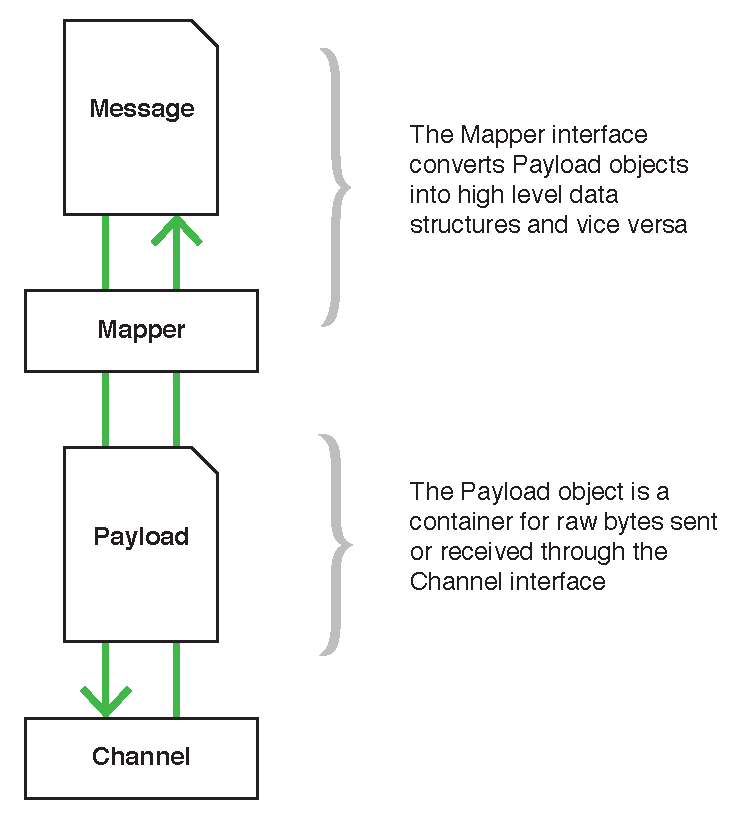
\includegraphics[width=0.6\textwidth]{imgs/mapper_payload.pdf}
\caption{Relationship between the \texttt{Channel}, \texttt{Payload},
\texttt{Mapper} and \texttt{Message} objects.}
\label{fig:channel.async}
\end{figure}

~\\
\lstset{language=Java}
\begin{lstlisting}[floatplacement=!hbt,caption=The Message
interface,label={lst:message}]
public interface Message {
    public String getType();

    public boolean hasField(String name);

    public Object getField(String name)
                throws IllegalArgumentException;

    public void setField(String name, Object value)
                throws IllegalArgumentException;

    public void appendElement(String name,Object element)
                throws IllegalArgumentException;

    public boolean validate();
}
\end{lstlisting}

The specific structure of a \texttt{Message} is defined by its type, which can
be queried through the \texttt{getType()} method. This property unequivocally
identifies the set of fields contained in a \texttt{Message} in terms of field
\textbf{name}, field \textbf{type} and field \textbf{qualifier}.

The field \textbf{name} is a textual attribute that uniquely identifies one
specific data item in the scope of a single \texttt{Message}. It can be used to
retrieve or set the value of a field through the \texttt{getField()} and
\texttt{setField()} methods respectively.

The \textbf{type} attribute defines the set of legal values that can be stored
in a field, together with the operations that are allowed on those values. It
is worth mentioning that this information is used to statically verify the type
safety of nearly all data management operations performed on a \texttt{Message}
(consult section~\ref{sec:components.script} for additional information). The
PerLa Middleware currently supports six primitive types:

\begin{itemize}

  \item \textbf{INTEGER}: a 32 bit signed two's complement integral data type

  \item \textbf{FLOAT}: a single-precision 32 bit IEEE 745 floating point

  \item \textbf{BOOLEAN}: a type with only two values, true or false

  \item \textbf{STRING}: a string of characters with UTF-16 encoding

  \item \textbf{TIMESTAMP}: a date with timezone, currently implemented using
      Java's \texttt{ZonedDateTime} class.

  \item \textbf{ID}: a unique label that identifies a single node connected in
      a PerLa managed network. The current implementation uses a 32 bit
      integer. 

\end{itemize}

Besides the data types presented above, fields can also be configured to hold
nested \texttt{Message}s. In this case, the type attribute must be set to the
particular type of \texttt{Message} that is to be stored in the field. 

The \textbf{qualifier} attribute is employed to define additional field
properties. It can be set to one of the following values:

\begin{itemize}

  \item \textbf{SIMPLE}: a normal field whose value can be altered and
      retrieved using the \texttt{setField()} and \texttt{getField()} methods
      respectively.

  \item \textbf{LIST}: a field that can hold multiple elements of the same
      type. New values can be added with the \texttt{appendElement()} method,
      and the entire list can be retrieved through the conventional
      \texttt{getField()} method. List-qualified fields preserve the order of
      insertion of the individual elements.

  \item \textbf{STATIC}: a field whose value is statically set when the
      \texttt{Message} type is declared. Any attempt to modify a
      statically-qualified field with either the \texttt{setField()} or the
      \texttt{appendElement()} methods will cause an exception to be thrown. It
      is important to note that static field values are set on a per-type
      basis; this means that all \texttt{Message}s of the same type will share
      the same field values for each static field (if any).
      
\end{itemize}


\subsection{Working with Messages: the Mapper interface}

\texttt{Message} objects are managed by the \texttt{Mapper} component. Its
interface, available in listing~\ref{lst:mapper}, groups all the
functionalities needed to handle a specific variety of structured information.
The one-to-one relationship between \texttt{Mapper}s and data types is
epitomized by the \texttt{getMessageType()} method, whose return value
indicates which \texttt{Message} class is supported by a particular
\texttt{Mapper}. This method is extensively employed by the Middleware to sift
through a collection of \texttt{Mapper}s, in order to find one that is best
suited for handling the information currently being processed.

~\\
\lstset{language=Java}
\begin{lstlisting}[floatplacement=!hbt,caption=The Mapper
interface,label={lst:mapper}]
public interface Mapper {

    public String getMessageType();

    public FieldDescriptor getFieldDescriptor(String name);

    public Collection<FieldDescriptor> getFieldDescriptors();

    public FpcMessage createMessage();

    public FpcMessage unmarshal(Payload payload);

    public Payload marshal(FpcMessage message);

}
\end{lstlisting}

Interactions with a \texttt{Mapper} usually begin with a call to the
\texttt{createMessage()} method, whose execution results in the creation of an
empty \texttt{Message} instance. Despite its unsuprising outcome, this method
draws once again our attention to the close relationship between
\texttt{Mapper}s and data types. Every \texttt{Mapper} instance is in fact
committed to the management of a precise class of information, hence all
\texttt{Message}s created with the \texttt{createMessage()} method will share
the same data type property, and, consequently, the same set of fields. The
interdependence between a \texttt{Mapper} and its assigned type is accentuated
even further by the \texttt{getFieldDescriptor()} and
\texttt{getFieldDescriptors()} methods, which can be used to analyze the
internal field structure characterizing all \texttt{Message} objects that the
\texttt{Mapper} creates. This introspective capability is extensively exploited
in the Execution Engine to check whether a \textit{Script} is type-safe or not
(see section~\ref{sec:components.script} for further details).

As explained in the introductory paragraphs of this section, \texttt{Message}
objects are a convenience introduced for simplifying data management operations
in the PerLa Middleware. They provide structured access to information, a
familiar set of primitive data types, and a selection of tools for combining
basic values into complex data structures. In spite of these advantages, the
\texttt{Message} interface is a high level abstraction that cannot be employed
where a \texttt{Payload} is expected, since its contents are not directly
accessible as a simple sequence of bytes; as a consequence, \texttt{Message}s
can't be used for any kind of I/O operation. This structural gap is bridged by
the \texttt{marshal()} and \texttt{unmarshal()} methods of the \texttt{Mapper}
interface. As can be seen by analyzing their respective signatures, these two
methods can be used to convert \texttt{Message} objects into \texttt{Payload}s
and vice-versa. This additional \texttt{Mapper} functionality brings to light
yet another aspect of the PerLa data management layer, namely its ability to
work with different representations of binary data.

Every \texttt{Mapper} is in fact created to support a single data format;
\texttt{JSONMapper} instances, for example, handle JSON-formatted byte streams,
whereas \texttt{URLEncodedMapper}s specialize in the conversion of URL-encoded
HTTP entities. The structure of the \texttt{Message}s created by a
\texttt{Mapper} and the data format they can be marshalled unto are not
orthogonal concerns, as the choice of a specific binary representation may
prevent the use of some of the previously discussed field attributes. The
URL-encoded format, for example, is defined as a flat collection of key-value
pairs, with no support for nested data structures; hence, the corresponding
\texttt{URLEncodedMapper} class could never be used to create and manage
\texttt{Message}s with nested fields. The close connection between a
\texttt{Message} and its corresponding binary format manifests itself in the
design of the \texttt{Mapper} component, specifically in the decision to
coalesce the marshalling/unmarshalling mechanism, and the more general
\texttt{Message} management methods (\texttt{createMessage()},
\texttt{getFieldDescriptors()}), under the same interface. The specific
methodology for creating \texttt{Mapper} objects, and for defining their
distinctive data format and \texttt{Message} type, will be subject of
additional discussion in the remainder of this chapter.

\begin{figure}[h!]
    \centering
    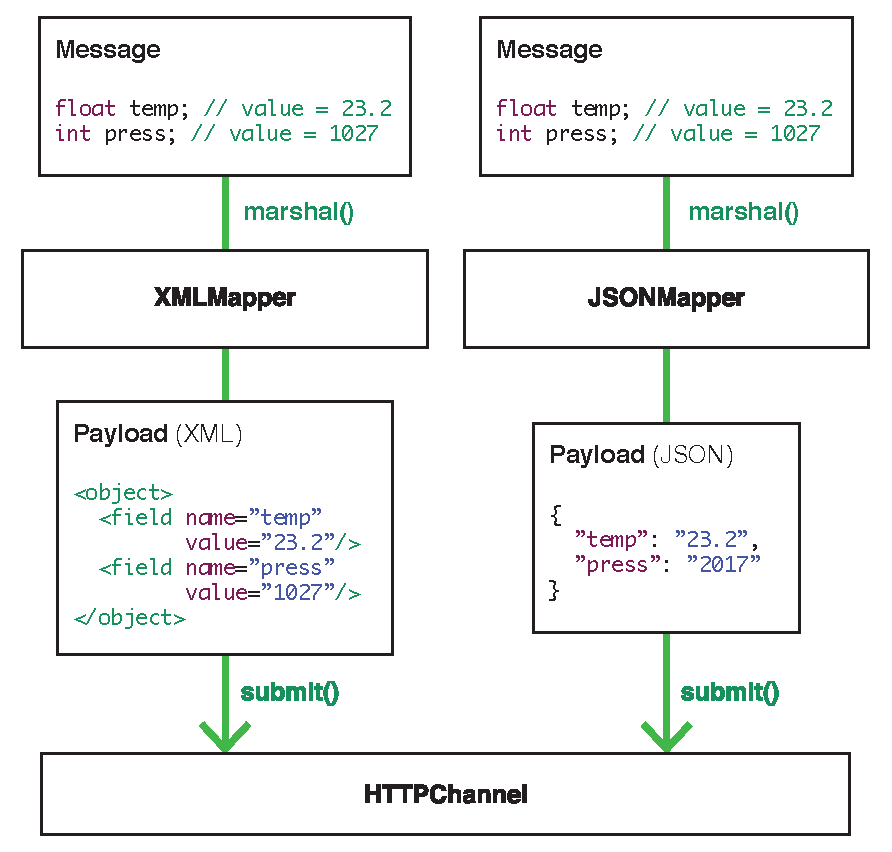
\includegraphics[scale=0.8]{imgs/mapper_channel.pdf}
    \caption{Using a single \texttt{Channel} to transmit data marshalled with
    different \texttt{Mapper}s}
    \label{fig:mapper_channel}
\end{figure}

Before this section comes to an end, it is worth putting into context the role
occupied by the \texttt{Mapper} inside the PerLa Middleware. The additional
decoupling provided by the \texttt{Mapper} builds over the pluggable
\texttt{Channel} interface, thus allowing the payload format to be selected
independently of the I/O stack.  This is an important characteristic of the
Middleware design, as even the simplest communication protocol usually requires
several \texttt{Message} structures, viz. several \texttt{Mapper}s, for
exchanging data between two endpoints.


\subsection{Creating Mappers and defining Message structures}

New \texttt{Mapper} objects are created by means of the \texttt{MapperFactory}
interface.

\lstset{language=Java}
\begin{lstlisting}[float,floatplacement=!hbt,caption=The Mapper Factory
interface,label={lst:mapperFactory}]
public interface MapperFactory {

    public Class<? extends MessageDescriptor>
        acceptedMessageDescriptorClass();

    public Mapper createMapper(MessageDescriptor descriptor,
        Map<String, Mapper> mapperMap, ClassPool classPool)
                    throws InvalidDeviceDescriptorException;

}
\end{lstlisting}

Its design follows the same concepts explained in previous sections; the
\texttt{acceptedMessageDescriptorClass()} method returns the type of
\texttt{MessageDescriptor} objects that can be used with the
\texttt{MapperFactory}, while the \texttt{createMapper()} method consumes a
\texttt{MessageDescriptor} to create a \texttt{Mapper}. However, differently
from all factory components described so far, the creation of a new object
calls for two additional parameters other than the descriptor itself: a
\texttt{ClassPool}, and a map of \texttt{Mapper}s. These extra items contain a
reference to previously built \texttt{Mapper}s, and can be used to check
whether nested \texttt{Message} fields are properly declared or not.

The \texttt{MapperFactory} interface is an additional extension point available
to PerLa users, and can be leveraged to introduce support for new binary
formats and information encoding schemes. As a consequence, every installation
of the Middleware will contain a wide variety of \texttt{MapperFactory}
implementations, each of which is dedicated to a single data format. Instances
of the previously introduced JSON and URL-Encoded mappers, for example, are
created by two distinct \texttt{MapperFactory} objects, namely
\texttt{JSONMapperFactory} and \texttt{URLEncodedMapperFactory}. This design is
a substantial improvement on the previous middleware architecture, as it
ensures that every \texttt{MapperFactory} object is responsible for managing
the quirks of only a single data format.

Moreover, every \texttt{MapperFactory} implementation is bundled with a custom
\texttt{MessageDescriptor} object, whose class name is exposed by the
aforementioned \texttt{acceptedMessageDescriptorClass()} method. The additional
complexity deriving from this design choice is more than made up for in type
safety and flexibility, as each different \texttt{MessageDescriptor} may be
implemented to closely represent the idiosyncratic characteristics of its
corresponding data format. A concrete example of this concept comes from the
\texttt{URLEncodedMessageDescriptor} class, which prevents the creation of
\texttt{Message}s that don't comply with the URL-encoded format by disallowing
non-primitive fields. Having multiple \texttt{MessageDescriptor}s also means
that different \texttt{Message}s are not forced to abide by the same set of
rules; the limits imposed on URL-encoded messages are not universal, and in
fact the \texttt{JSONMessageDescriptor} refrains from applying them.
Furthermore, \texttt{MessageDescriptor} objects can adopt a custom lexicon for
expressing the PerLa-specific concepts of \textit{message}, \textit{field} and
\textit{field type}. Take for example listings \ref{lst:jsonmessage} and
\ref{lst:urlencodedmessage}. These two XML snippets show how the vocabulary
employed in message declarations varies with the data format (field are dubbed
\textit{member} in JSON, and \textit{parameter} in URL-Encoded strings). Using
a terminology that best suits the actual data format makes \texttt{Message}
declarations idiomatic, reminiscent of the corresponding real-world objects and
therefore easier to use.

\lstset{language=XML}
\begin{lstlisting}[float,floatplacement=!hbt,caption={A compound JSON message
        declared using the JSONMessageDescriptor (XML notation). Note that the
        data type of all fields inside \texttt{weather} message is a reference
        to a previously declared \texttt{Message}.
},label={lst:jsonmessage}]

<js:object id="coord">
    <js:member name="lon" type="string"/>
    <js:member name="lat" type="string"/>
</js:object>

<js:object id="main">
        <js:member name="temp" type="float"/>
        <js:member name="pressure" type="float"/>
        <js:member name="humidity" type="float"/>
        <js:member name="temp_min" type="float"/>
        <js:member name="temp_max" type="float"/>
</js:object>

<js:object id="wind">
        <js:member name="speed" type="float"/>
        <js:member name="deg" type="float"/>
</js:object>

<js:object id="weather">
        <js:member name="coord" type="coord"/>
        <js:member name="main" type="main"/>
        <js:member name="wind" type="wind"/>
</js:object>

\end{lstlisting}


\lstset{language=XML}
\begin{lstlisting}[float,floatplacement=!hbt,caption={An URLEncoded message
declaration. Thanks to the custom \texttt{URLEncodedMessageDescriptor}, trying
to create a non-primitive field results in an exception. Note the custom
\texttt{format} attribute on the timestamp field, which is employed to define
the encoding format for dates and times},label={lst:urlencodedmessage}]

<ue:message id="urlencoded_message">
        <ue:parameter name="temperature" type="float"/>
        <ue:parameter name="pressure" type="float"/>
        <ue:parameter name="location" type="string"/>
        <ue:parameter name="key" qualifier="static" type="integer" value="5"/>
        <ue:parameter name="timestamp" type="timestamp" format="d MMM uuuu HH:mm"/>
</ue:message>

\end{lstlisting}


\subsection{Managing multiple message types}

It is not uncommon for a single device to communicate using multiple message
formats; developers may choose to encapsulate different information inside
different data structures, which the receiver must correctly identify to
decipher their contents. In such cases, every \texttt{Message} exchanged
between the two endpoints is tagged with a data type value, i.e., a common
field that advertises the type of information being transferred. This technique
is widespread among firmware developers, since it can be easily implemented
with most programming languages (C/C++ support it by design through
\texttt{tagged unions}).

The PerLa Middleware implements various techniques to cope with sensor nodes
that communicate using multiple message formats. First of all, only the data
structures that can actually be received are considered when unmarshalling a
byte stream; if under the current conditions a device only sends a subset of
its available message types, then the Middleware can immediately rule out the
unmatching ones. As it will be discussed later, a collection of expected data
formats is automatically curated by the \texttt{FPC} by cross-comparing
information excerpted from the Device Descriptor with the current device
status. It should be clear that this technique alone is not enough to cover all
practical use cases, as it falls short as soon as a device starts sending two
or more message varieties concurrenty; in such scenarios, PerLa needs to search
for clues that will help it recognize how the bytes being received are
structured. These clues take the form of \textit{static} fields. When faced
with an ambiguous situation, the \texttt{FPC} will try unmarshal the bytes
received into all expected data types. A congruency check will then be
performed on the resulting \texttt{Message}s: the data can be considered
correctly decoded only when all its static fields match the corresponding
Device Descriptor declaration. This methodology can be employed to interact
with sensor nodes that make use of tagged data structures. 


\section{Data management: Scripts}
\label{sec:components.script}

\texttt{Channel}s, \texttt{Payload}s, \texttt{Mapper}s and \texttt{Message}s
are the core components used by PerLa to exchange data with nodes of a
Pervasive System. They provide the supporting infrastructure through which
information can be serialized, transmitted and faithfully reconstructed at the
receiving endpoint. Taken together, these components implement an adaptable
transport layer, whose features can be tailored around each device connected to
the Middleware: combine a \texttt{HTTPChannel} with a \texttt{JSONMapper} to
obtain a network stack for RESTful services; swap the data layer with an
\texttt{XMLMapper} if the format changes; add a \texttt{ZigbeeChannel} and a
\texttt{StructMapper} to communicate with low-powered devices in a mesh
network. In spite of their individual capabilities, all these components are
not enough to glean information from a Sensor Network. The interaction with a
sensor node requires far more than a transport layer; in fact it can only occur
when data transfer operations follow a strict set of rules, i.e., an
\textit{application protocol}. \texttt{Channel}s, \texttt{Mapper}s and
\texttt{Message}s provide no more than the basic building blocks needed for the
interaction, but their use is to be tightly orchestrated before any purposeful
exchange of information can take place.

PerLa \textit{Script}s, just referred as \textit{Script}s in the remainder of
this document, implement the kind of structural scaffolding required to
organize a series of primitive data management operations into a
self-contained, reusable procedure. Their purpose in the PerLa Middleware is
twofold: first, to issue commands that conform to the specific protocols used
in a Pervasive Systems; second, to act as an impedance matcher between the
structured information collected from a sensor network and the record-oriented
output of an \texttt{FPC}. The PerLa scripting language is one of the most
distinctive features of the new Middleware design; a procedural programming
tool that can be used to complement and enrich the declarative nature of the
Device Descriptor. \textit{Script}s improve the reusability of all existing and
future Middleware components, as they can be used to adjust the output of a
computation before it's used as the input of another one.

\begin{figure}[h!]
    \centering
    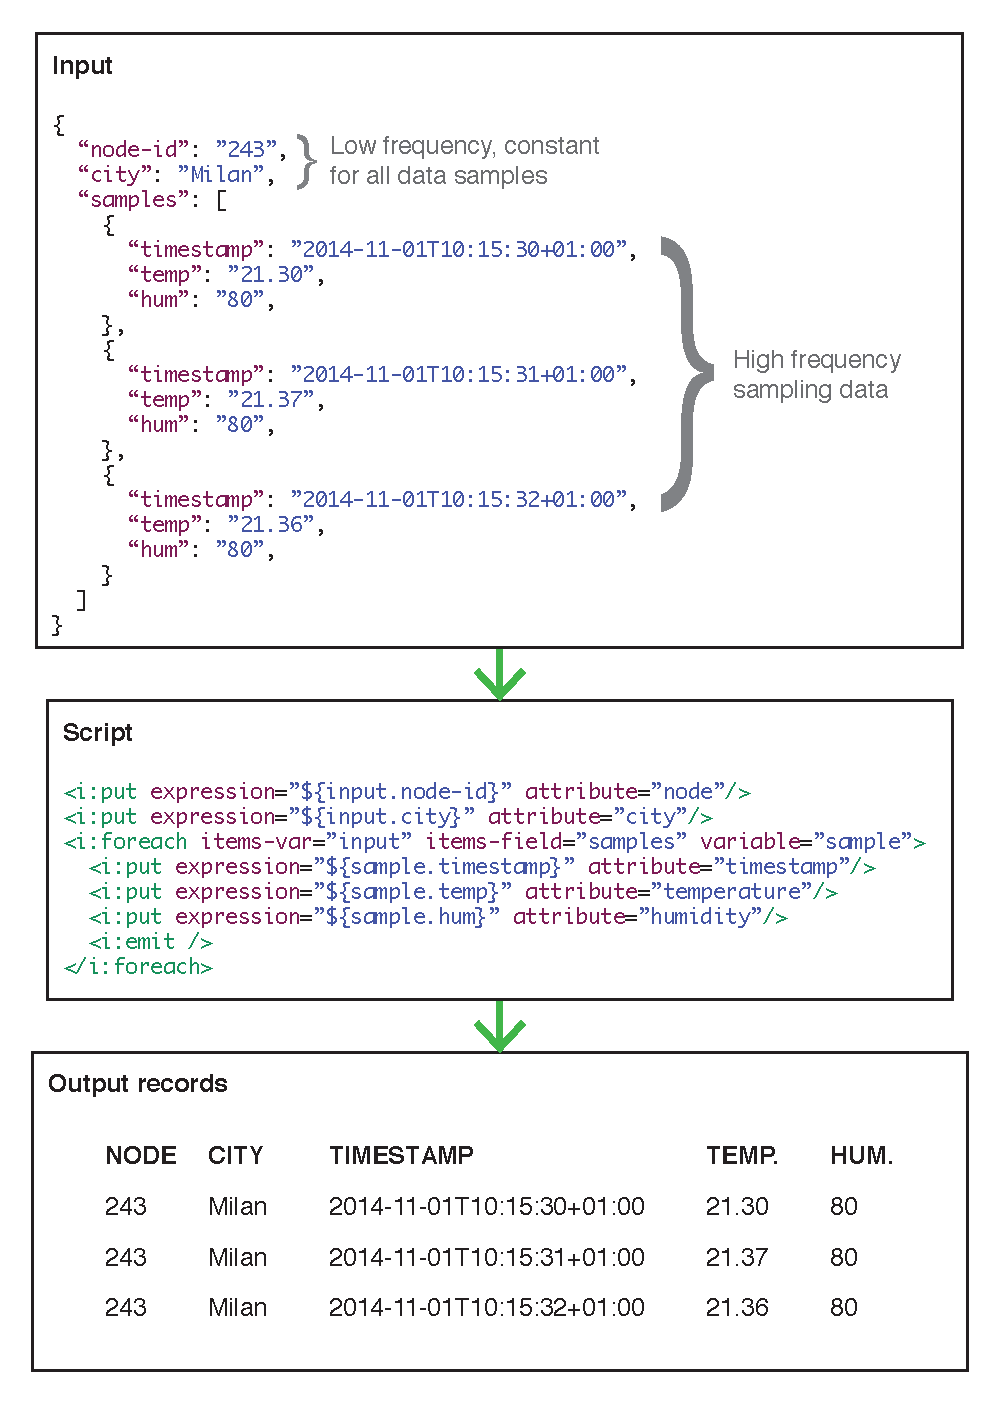
\includegraphics[scale=0.8]{imgs/script_unrolling.pdf}
    \caption{Flattening the content of a nested JSON data structure with a
    PerLa \texttt{Script}}
    \label{fig:script_unrolling}
\end{figure}

An archetypal example of this concept is given in
figure~\ref{fig:script_unrolling}. This \textit{Script} solves a recurring
impedance matching problem: a device that stores multiple samples into a common
data structure, and sends them with a single transmission in order to conserve
battery power. The result of such aggregation can't be coerced into a sequence
of records as-is, as more often than not it contains a mixture of both high
frequency and low frequency information (and indeed it does in the current
example). The PerLa scripting language can be used to unroll the high frequency
content, complement it with the information that remains constant for all
samples, and output the resulting records one by one; all without having to
resort to a bespoken \texttt{Mapper} implementation, as it would prove
necessary if the former Middleware were used instead. Moreover, this same
script can be easily employed to handle similar aggregation patterns with
little or none modifications, as it doesn't depend on any particular
\texttt{Channel}, \texttt{Mapper} or \texttt{Message} implementation.

PerLa \textit{Scripts} are also used to address minor compatibility problems
that may arise when authoring new Device Descriptors; they can wrap an existing
Middleware component and adapt its behaviour to handle an unforseen usage
scenario, convert information between different units of measure, alter a
\texttt{Message} before it is sent to the intended recipient, or compute
aggregations. It is important to note that \textit{Scripts} are slower than
pure Java code; an excessive usage in data intensive, real-time applications
should be carefully avoided, as it may negatively affect the performance of the
entire Middleware. End users are therefore invited to thoroughly test and
benchmark their Device Descriptors to eliminate any potential bottleneck before
deployment.


\subsection{Anatomy of a PerLa Script}

PerLa \texttt{Script} is a full-fledged imperative programming language
composed of data management instructions, control flow statements and a
powerful expression language. Procedures written in PerLa \texttt{Script} are
processed by the \texttt{Script Engine}, a Middleware module that reads,
interprets and executes script instructions. Instructions are specified using a
proprietary XML syntax, specifically designed to allow PerLa \texttt{Scripts}
to be directly embedded in a Device Descriptor. Conflicts with potentially
similar XML tags and attributes are avoided through the
\texttt{http://perla.dei.org/device/instructions} namespace, which is commonly
associated with the ``\texttt{<i:}'' prefix. PerLa developers are invited to
follow this convention, as the use of a different namespace prefix may create
confusion among end users and future Device Descriptor maintainers. 

Every \texttt{Script} instruction is composed of a \textit{name}, a textual
property that identifies a specific type of computation, and a list of
\textit{parameters}, name-value pairs that customize its runtime behaviour.
With the exception of the \texttt{submit} instruction, whose unconventional
characteristics are described in the remainder of this section, parameters are
always defined using the standard XML attribute syntax.  PerLa \texttt{Scripts}
currently support two different types of parameter values: \textit{literals}
and \textit{expressions}. Literals are simple textual strings, which are used
as-is by the execution engine to express constant concepts like variable names
or immutable values. Expressions, on the other hand, are combinations of
variables, operators, functions and constants, whose evaluation produces a new
result value. Differently from literals, expressions are prefixed by the \$
sign and enclosed in curly braces (\lstinline!${ ... }!); this cue is employed
by the execution engine to determine whether an instruction parameter has to be
pre-processed or not prior to being used.  Expressions can be used to perform
the following actions:

\begin{itemize}
        
    \item Arithmetic operations (sum, subtration, product, division, modulo)

    \item Logical operations (or, and, not)

    \item Comparisons (\lstinline$<, >, !=, <=, >=$)

    \item Access \texttt{Message} fields (dot operator). Multiple dot operators
        may be applied in succession to access a specific value buried inside a
        complex data structure (e.g., the expression
        \lstinline!${result.environment.temperature}! is used to traverse 3
        nesting levels).

    \item Retrieve \texttt{Script} arguments through the built-in \texttt{args}
        associative array. This feature can be leveraged to create parametric
        \texttt{Script}s that dynamically adapt to the user's requests.

\end{itemize}

Whether a certain parameter can be specified as a literal, as an expression, or
both, depends entirely on the instruction in which it is employed. This
information, along with other useful details regarding the PerLa Scripting
language, is available in the following instruction compendium.

\subsubsection{\texttt{var} instruction}

\textbf{Description}

Declares a new variable. This instruction requires two mandatory parameters:

\begin{itemize}

    \item \textbf{name:} The variable name, namely a textual identifier used to
        reference the variable in later instructions. It must be unique in the
        scope of a single script.

    \item \textbf{type:} The type of data that can be stored inside the newly
        created variable. It can be set to one of the six PerLa primitive data
        types, or to a user-defined  message type.

\end{itemize}

\textbf{Usage examples}

Creates a new variable named \texttt{count} of primitive type \texttt{integer}.

\lstset{language=XML}
\begin{lstlisting}
<i:var name="count" type="integer"/>
\end{lstlisting}

Creates a new variable named \texttt{cmd} of complex type
\texttt{node\_command}, whose declaration is omitted for brevity reasons.

\lstset{language=XML}
\begin{lstlisting}
<i:var name="cmd" type="node_command"/>
\end{lstlisting}

\subsection{\texttt{set} instruction}

\textbf{Description}

Sets the contents of a variable to a new value. The optional \texttt{field}
parameter can be used whenever the user needs to modify a specific field in a
variable of complex type.

\begin{itemize}

    \item \textbf{variable:} Name of the variable to be modified.

    \item \textbf{field (optional):} An optional parameter that can be used to
        select the specific field to set in a variable of complex type.

    \item \textbf{value:} The new value of the variable. This parameter may
        be either a literal value or an expression.

\end{itemize}

\textbf{Usage examples}

Sets the previously defined \texttt{count} variable to the literal value \texttt{5}.

\lstset{language=XML}
\begin{lstlisting}
<i:set variable="count" value="5"/>
\end{lstlisting}

Sets the field \texttt{operation} of the previously defined \texttt{cmd}
variable to the literal value \texttt{sample}.

\lstset{language=XML}
\begin{lstlisting}
<i:set variable="cmd" field="operation" value="sample"/>
\end{lstlisting}

Converts a temperature reading from Celsius to Fahreheit degrees, and stores it
in the \texttt{temp\_f} field of a hypothetical variable named \texttt{result}.

\lstset{language=XML}
\begin{lstlisting}
<i:set variable="result" field="temp_f"
    value="${result.temp_c * 9/5 + 32}"/>
\end{lstlisting}

Deep copy. The content of the source variable is accessed with the
``\lstinline!${original}!'' expression.

\lstset{language=XML}
\begin{lstlisting}
<i:set variable="copy" value="${original}"/>
\end{lstlisting}


\subsubsection{\texttt{append} instruction}

\textbf{Description}

Appends a new element to the end of a list-qualified field.

\begin{itemize}

    \item \textbf{variable:} Name of the variable to be modified.
    
    \item \textbf{field:} Name of the list-qualified field to which the new
        value is to be appended.

    \item \textbf{value:} The new value to be inserted. This parameter may
        either be a literal value or an expression.

\end{itemize}

\textbf{Usage examples}

Appends the literal value ``\texttt{5}'' to a list field.

\lstset{language=XML}
\begin{lstlisting}
<i:append variable="result" field="temp_list" value="5"/>
\end{lstlisting}


\subsubsection{\texttt{submit} instruction}

\textbf{Description}

Submits an \texttt{IORequest} on a \texttt{Channel}. This instruction supports
the following parameters:

\begin{itemize}

    \item \textbf{request:} Identifier of the \texttt{IORequest} to be
        submitted.

    \item \textbf{channel:} Identifier of the \texttt{Channel} on which the
        request has to be submitted

    \item \textbf{variable (optional):} Name of the variable used to store the
        result of the I/O operation. If present, the complementary
        \textbf{type} parameter must be set. It is important to note that the
        result variable is automatically declared by the \texttt{submit}
        instruction; therefore, the final user must not create it with an
        explicitly \texttt{var} instruction.

    \item \textbf{type (optional):} Type of the variable used to store the
        result of the I/O operation. Its presence is subordinated to the
        aforementioned \textbf{type} parameter.

\end{itemize}

Additional \texttt{IORequest} parameters may be specified by supplying an
appropriate list of \texttt{param} XML tags, each of which must contain the
name of the parameter being set, and a reference to a variable containing the
desired value (see the usage example section below for further syntax
information). Upon submission, this instruction will automatically handle every
\texttt{Mapper} operation required to convert the parameter value into a
\texttt{Payload} object suited to the I/O operation.

\textbf{Usage examples}

Basic usage, submits the ``\texttt{start\_sampling}'' request to a
\texttt{SerialChannel}. All information received during the I/O operation is
discarded, since no result variable is specified for this instruction.

\lstset{language=XML}
\begin{lstlisting}
<i:submit request="start_sampling" channel="serial"/>
\end{lstlisting}

Submits the ``\texttt{get\_data}'' request to a \texttt{HTTPChannel}. All
bytes received from the remote server are stored in the \texttt{result}
variable.

\lstset{language=XML}
\begin{lstlisting}
<i:submit request="get_data" channel="http"
  variable="result" type="json_result"/>
\end{lstlisting}

Submits the ``\texttt{send\_command}'' request to a \texttt{SerialChannel}.
The \texttt{command} variable is set as an \texttt{IORequest} parameter.

\lstset{language=XML}
\begin{lstlisting}
<i:submit request="get_data" channel="http">
  <i:param name="payload" variable="command"/>
</i:submit>
\end{lstlisting}


\subsubsection{\texttt{stop} instruction}

\textbf{Description}

Stops the \texttt{Script}. This instruction is usually employed in conjunction
with the \texttt{if} control structure to implement advanced halt conditions
based on information available only at runtime.

\textbf{Usage example}

Immediately stops the execution of the \texttt{Script}.

\lstset{language=XML}
\begin{lstlisting}
<i:stop/>
\end{lstlisting}

Guarded stop. Halts the execution of the \texttt{Script} only when a certain
condition holds true.

\lstset{language=XML}
\begin{lstlisting}
<i:if condition="${temp_c > 25}"> 
  <i:then>
    <i:stop/>
  </i:then>
</i:if>
\end{lstlisting}


\subsubsection{\texttt{error} instruction}

\textbf{Description}

Aborts the \texttt{Script}, signalling an abnormal execution condition. This
instruction must be supplied with a \textbf{message} parameter that indicates
the cause of failure. Similarly to the \texttt{stop} instruction,
\texttt{error} invocations are commonly guarded by an \texttt{if} control
structure to implement advanced error management behaviours.

\textbf{Usage examples}

The following code excerpt throws an error when the humidity level falls
outside the acceptable range. This example combines the \texttt{stop} and
\texttt{error} instructions to demonstrate a typical PerLa \texttt{Script}
error management pattern.

\lstset{language=XML}
\begin{lstlisting}
<i:if condition="${humidity >= 0 && humidity <= 100}"> 
  <i:then>
    <i:put expression="${humidity}" attribute="humidity"/>
    <i:emit/>
    <i:stop/>
  </i:then>
  <i:else>
    <i:error message="humidity out of range"/>
  </i:else>
</i:if>
\end{lstlisting}


\subsubsection{\texttt{put} instruction}

\textbf{Description}

Adds a field into the staging area, viz. a temporary storage location used
for the incremental creation of new output records. This instruction requires
two mandatory parameters:

\begin{itemize}

    \item \textbf{attribute:} Name of the attribute corresponding to the value
        being added in the staging area. The purpose of this parameter is
        twofold: first, it defines the name through which the new data can be
        retrieved (record field names always correspond to device attribute
        names); second, it is used to confirm that the value being added in the
        staging area has the correct data type (record field types always
        correspond to device attribute types).

    \item \textbf{expression:} Value of the new record field.

\end{itemize}

This instruction is intended to be called multiple times in the lifetime of a
single \texttt{Script} execution, as a single \texttt{put} operation can only
be used to set one record field at a time. As soon as all the desired values
are staged, the content of the entired staging area can be flushed into a new
record by means of the \texttt{emit} instruction.

It is worth noting that the content of the staging area is not deleted once
\texttt{emit} is invoked. Though this may seem counterintuitive or even
undesirable, such behaviour allows for a simpler and more efficient management
of aggregated data. The ability to retain all field values set with previous
invocations of the \texttt{put} instruction is key to the example of
figure~\ref{fig:script_unrolling}, where low frequency information --- namely
the \textit{name-id} and the \textit{city} records --- is set only once, and
only the high-frequency samples are continuously replaced with new calls to the
\texttt{put} instruction. This optimization technique would not be possible if
the staging area were not provided with the aforementioned memory-retaining
mechanism.

\textbf{Usage Examples}

Refer to section~\ref{sec:emit_instruction} for combined usage examples of the
instructions \texttt{put} and \texttt{emit}.


\subsubsection{\texttt{emit} instruction}
\label{sec:emit_instruction}

\textbf{Description}

Creates a new record using the field values stored in the staging area. All
records created by the \texttt{emit} instruction are released to the user only
if the \texttt{Script} terminates without errors.

\textbf{Usage Examples}

Creates a record containing two literal fields.

\lstset{language=XML}
\begin{lstlisting}
<i:put attribute="temperature" expression="25"/>
<i:put attribute="humidity" expression="85"/>
<i:emit/>
\end{lstlisting}

Maps a flat data structure into a record. Differently from the previous
example, record values are dynamically read from the \texttt{sample} variable,
hypothetically received from a remote sensor node.

\lstset{language=XML}
\begin{lstlisting}
<i:put attribute="temperature" expression="${sample.temperature}"/>
<i:put attribute="humidity" expression="${sample.humidity}"/>
<i:put attribute="timestamp" expression="${sample.timestamp}"/>
<i:emit/>
\end{lstlisting}

\texttt{Script} expressions can also be used to create new record values at
runtime. In the following code snippet, a simple conversion formula is employed
to derive the \texttt{temp\_fahrenheit} record field from other information
sent by the sensor node.

\lstset{language=XML}
\begin{lstlisting}
<i:put attribute="temp_centigrade" expression="${sample.temp_cent}"/>
<i:put attribute="temp_fahrenheit"
  expression="${sample.temp_centigrade * 9/5 + 32}"/>
<i:put attribute="humidity" expression="${sample.humidity}"/>
<i:put attribute="timestamp" expression="${sample.timestamp}"/>
<i:emit/>
\end{lstlisting}

Looping over multiple samples stored in a list. The following example creates a
new record for each element contained in the \texttt{data.samples} field. 

\lstset{language=XML}
\begin{lstlisting}
<i:foreach items-var="data" items-field="samples" variable="sample">
  <i:put expression="${sample.timestamp}" attribute="timestamp"/>
  <i:put expression="${sample.temp}" attribute="temperature"/>
  <i:put expression="${sample.hum}" attribute="humidity"/>
  <i:emit/>
</i:foreach>
\end{lstlisting}

Exploiting the characteristic memory-retention feature of the \texttt{put}
instruction to efficiently combine high-frequency and low-frequency
information. Note that the \texttt{node} and \texttt{city} fields are staged
only once, while all other fast changing information requires the execution of
a \texttt{put} instruction for each list element.

\lstset{language=XML}
\begin{lstlisting}
<i:put expression="${input.node-id}" attribute="node"/>
<i:put expression="${input.city}" attribute="city"/>
<i:foreach items-var="input" items-field="samples" variable="sample">
  <i:put expression="${sample.timestamp}" attribute="timestamp"/>
  <i:put expression="${sample.temp}" attribute="temperature"/>
  <i:put expression="${sample.hum}" attribute="humidity"/>
<i:emit />
</i:foreach> 
\end{lstlisting}

\subsubsection{\texttt{if} control structure}

\textbf{Description}

A conditional control structure for executing different \texttt{Script} branches
depending on whether a user-specified \textbf{condition} expression evaluates
to true or false.

\textbf{Usage example}

\texttt{If..then} example. Sets the variable \texttt{alarm} to TRUE when the
temperature rises above 25\degree~C.

\lstset{language=XML}
\begin{lstlisting}
<i:if condition="${temp_c > 25}"> 
  <i:then>
    <i:set variable="alarm" value="true"/>
  </i:then>
</i:if>
\end{lstlisting}

\texttt{If..then..else} example. Sets the variable \texttt{tropical} to TRUE
when the temperature rises above 30\degree~C and the humidity is greater than
90\%, to false otherwise.

\lstset{language=XML}
\begin{lstlisting}
<i:if condition="${temp_c > 25 && hum > 90}"> 
  <i:then>
    <i:set variable="tropical" value="true"/>
  </i:then>
  <i:else>
    <i:set variable="tropical" value="true"/>
  </i:else>
</i:if>
\end{lstlisting}


\subsubsection{\texttt{foreach} control structure}

\textbf{Description}

A control structure for traversing list-qualified \texttt{Message} fields. It
can be used to repeat a given block of code for every element of a collection.
The \texttt{foreach} control structure supports the following parameters:

\begin{itemize}

    \item \textbf{items-var:} Name of the source variable.

    \item \textbf{items-field:} Name of the source field, namely the
        list-qualified field inside the \textbf{items-var} on which to loop
        over.

    \item \textbf{variable:} Name of the variable through which the current
        item is exposed.

    \item \textbf{index (optional):} Index of the current item.

\end{itemize}

\textbf{Usage examples}

Computing the average of all temperatures received from a remote sensor node.

\lstset{language=XML}
\begin{lstlisting}
<i:var name="count" type="integer"/>
<i:set variable="count" value="0"/> 
<i:var name="avg" type="float"/>
<i:set variable="avg" value="0"/>
<i:foreach items-var="data" items-field="samples" variable="sample">
  <i:set variable="avg" value="${avg + sample.temperature}"/>
  <i:set variable="count" value="${count + 1}"/>
</i:foreach>
<i:set variable="avg" value="${avg / cont}"/>
\end{lstlisting}

\subsection{Script Engine architecture and execution model}

The \texttt{Script Engine} is the Middleware component responsible for the
execution of PerLa \texttt{Scripts}. It is currently implemented as a program
interpreter that parses and executes an intermediate PerLa \texttt{Script}
representation generated by the \texttt{FPCFactory}, dubbed SIR (Script
Intermediate Representation). SIR programs are directed graphs, where each node
is an instruction, and each arc is a potential evolution of the program status;
thus, SIR-encoded \texttt{Scripts} can be run by simply traversing the source
data structure until a \texttt{stop} instruction is encountered, or an error is
thrown. Thanks to this intermediate representation, the \texttt{Script Engine}
architecture is lean and efficient; the core execution loop need not be
concerned with the continuous interpretation of textual instructions or with
complex error-checking procedures, as these two operations are only performed
once, by the \texttt{FPCFactory}, when a \texttt{Script} is translated in its
corresponding SIR form. Moreover, as a result of the additional decoupling
provided by this intermediate code representation, the introduction of a new
PerLa \texttt{Script} format does not entail any modification to the
\texttt{Script Engine}, as long as a suitable SIR translator is provided for
the new syntax.

\begin{figure}[h!]
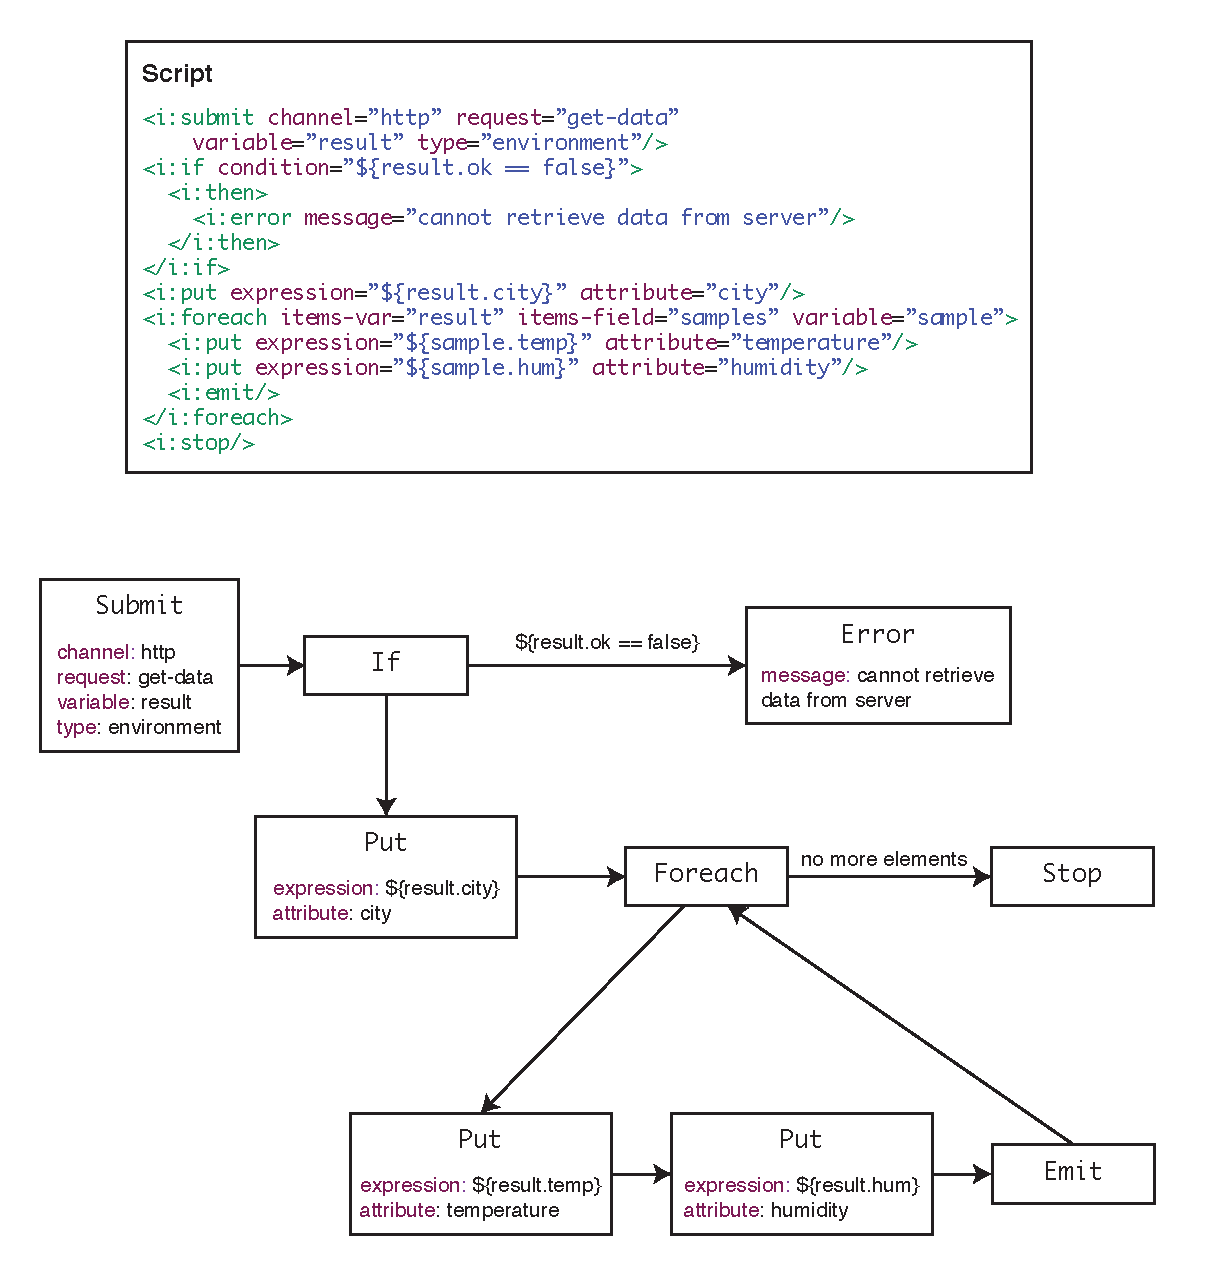
\includegraphics[width=\textwidth]{imgs/script_sir.pdf}
\caption{A PerLa \texttt{Script} and its corresponding SIR representation}
\end{figure}

Once started, PerLa \texttt{Scripts} are sandboxed in a dedicated thread of
execution. For better isolation, the current status of each running
\texttt{Script} instance is stored inside a private \texttt{ExecutionContext}
object, which contains the following elements:

\begin{itemize}

    \item \textbf{Program Counter:} A reference to the current instruction;

    \item \textbf{Variable Map:} An associative array that stores the current
        value of all declared variables;

    \item \textbf{Record staging area:} Temporary working area used to create
        new records;

    \item \textbf{Output records:} List of records to be returned when a
        \texttt{stop} instruction is encountered. 

\end{itemize}

This design ensures that all changes a single \texttt{Script} makes to its
environment will remain private, that its status won't be altered by any
other rogue routine, and that several \texttt{Scripts} can run simultaneously
without interfering with each other.

The execution of a \texttt{Script} is always subordinated to an external event,
like the submission of a new user request or the arrival of information from a
sensing device. In particular, PerLa \texttt{Scripts} associated with the
management of sensor data tend to run frequently and for a relatively short
period of time, as their execution is triggered by each sample collected from
the sensing network. To better cope with such usage scenario, the
\texttt{Script Engine} implements a thread caching mechanism that reduces
memory usage and startup times by reclaiming the runtime environment of each
terminated \texttt{Script}, and repurposing it for a new execution. This
caching technique greatly reduces the overall number of objects allocated by
the Java Virtual Machine, and guarantees that the overhead due to the
initialization of new \texttt{ExecutionContext} instances is shared between
multiple \texttt{Script} runs.

Moreover, the \texttt{Script Engine} can preemptively pause I/O bound
computations to optimize the usage of available system resources. This feature,
implemented by leveraging the asynchronous I/O design of the PerLa Middleware,
is totally transparent to the \texttt{Script} developer, who should not worry
with matters of concurrent programming; \texttt{Scripts} are automatically
paused after an \texttt{IORequest} is submitted to a \texttt{Channel}, and
their execution resumes as soon as the I/O activity terminates. These
two operations --- pause and resume --- are performed within the
\texttt{submit} instruction, which interrupts the \texttt{Script} after
an I/O request is submitted, and restarts it once the associated response is
available.


\section{Putting it all together: the FPC}

The \texttt{FPC} (Functionality Proxy Component) is the main data access
interface available to the PerLa Middleware. Its chief duty is to provide a
high-level abstraction of a Pervasive System by exposing the functionalities of
all devices of the network through a single consistent API. Every instance of
the PerLa Middleware hosts multiple \texttt{FPCs}, one for each sensing node.
This one-to-one relationship --- the fulcrum of the PerLa philosophy --- is a
fundamental architectural feature that endows the Middleware with utmost
flexibility and the finest granularity of control, as it presents final users
with the possibility to manage heterogeneous networks of sensing devices, down
to the single node, through a uniform set of high-level functions.

\begin{figure}[h!]
\center
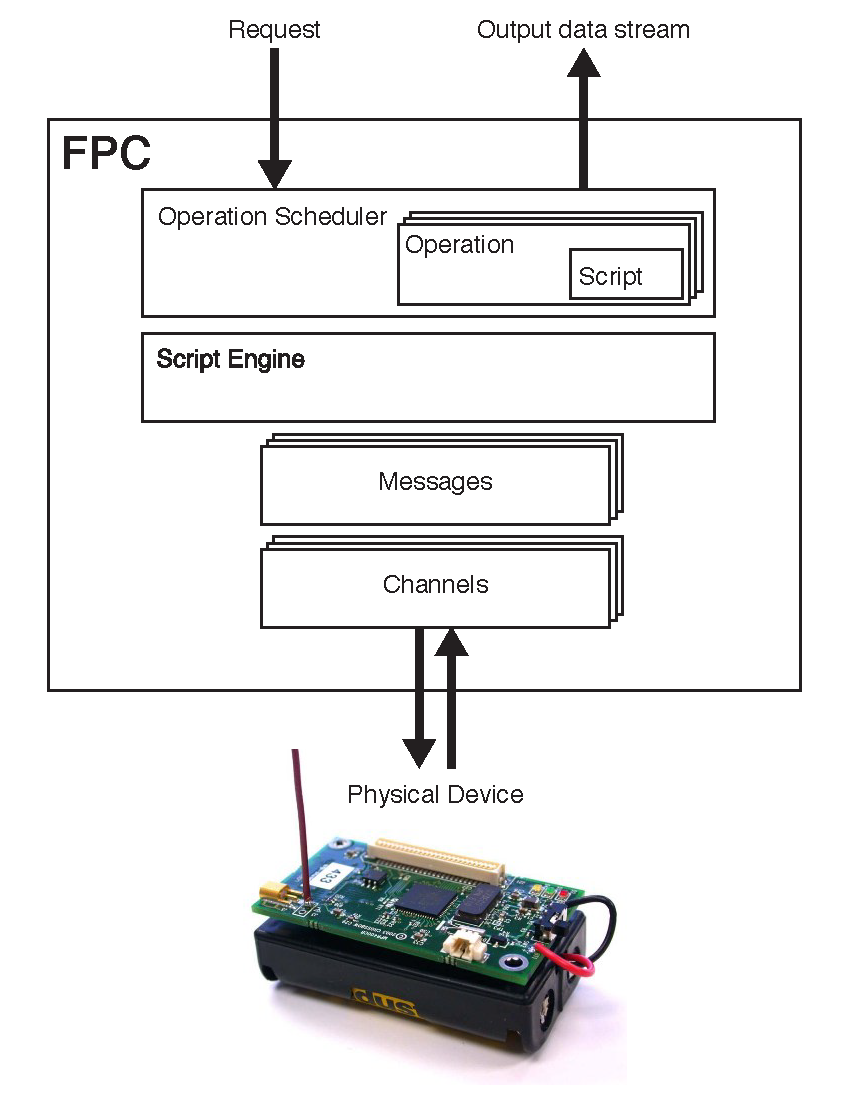
\includegraphics[width=0.6\textwidth]{imgs/fpc.pdf}
\caption{Internal structure of the Functionality Proxy Component}
\label{fig:fpc}
\end{figure}

\texttt{FPCs} are created from the composition of all Middleware components
described in the former sections of this chapter. As shown in
figure~\ref{fig:fpc}, these software modules are complemented by a set of
\texttt{Operations} and an \texttt{Operation Scheduler}. An \texttt{Operation}
is a collection of \texttt{Scripts} committed to the management of a well
defined aspect of an endpoint device, such as the retrieval of a specific data
sample at periodic intervals of time. In total, there are four different
\texttt{Operation} types available in the PerLa Middleware, each of which
corresponds to a \texttt{FPC} action (get, set, periodic sampling and
asynchronous event handling). Each of these \texttt{Operations} is associated
with the list of device \texttt{Attribute} that can be modified or generated
with it; this list is automatically inferred by the PerLa Middleware by
analyzing the associated data access \texttt{Scripts}.

\subsubsection{Get Operation}

A single \texttt{Script} that retrieves information from the remote device. It
can be used to perform a single-shot sampling operation or to read software
parameters stored on the connected endpoint.

This \texttt{Operation} type is introduced by the \lstinline!<get>! XML tag,
and contains a single PerLa \texttt{Script} that is responsible for connecting
with the remote device, retrieving the information requested by the user, and
creating an output record. The following example shows a textbook
implementation of the \texttt{Get Operation}, which demonstrates how all the
aforementioned operations can be performed in a few lines of PerLa
\texttt{Script}.

\lstset{language=XML}
\begin{lstlisting}
<get id="single-temp-sample">
  <i:submit request="temperature-request" channel="serial"
            variable="result" type="temperature-msg"/>
  <i:put expression="${result.temperature}" attribute="temperature"/>
  <i:emit/>
</get>
\end{lstlisting}

\subsubsection{Set Operation}

A single \texttt{Script} that sends information to the controlled device. It
can be used to dispatch commands, activate mechanisms, or change software
parameters on a remote sensing node.

All \texttt{Set Operation} \texttt{Scripts} must be enclosed in a
\lstinline!<set>! XML tag, and are required to define a series of actions
resulting in the transmission of data to the remote device. An example of this
\texttt{Operation} is available in the code excerpt below, which retrieves the
current time from a parameter passed by the \texttt{FPC} user
(\lstinline!arg['timestamp']!), and delivers it by means of a
\texttt{SerialChannel}.

\lstset{language=XML}
\begin{lstlisting}
<set id="set-clock">
  <i:create variable="settings" type="settings-msg"/>
  <i:set variable="settings" field="time" value="${arg['timestamp']}"/>
  <i:submit request="send-settings" channel="serial">
    <i:param name="payload" variable="settings"/>
  </i:submit>
</set>
\end{lstlisting}

\subsubsection{Periodic Operation}

A collection of \texttt{Scripts} for managing an unattended, periodic stream of
information. The \texttt{Periodic Operation} is more complicated than previous
\texttt{Operation} types, both from a syntactic and an operative point of view,
as it requires the device developer to specify three different classes of
\texttt{Scripts}.

The first of these is the \lstinline!<start>! \texttt{Script}, which is
employed to initialize the sampling operation. It normally contains a series of
instruction that parse the signal rate requested by the user, configure the
device to start the sampling operation, and handle potential error conditions.
By default, the sampling period exposed to the \texttt{Script} by means of the
\lstinline!arg['period']! argument is expressed in milliseconds; it is the
developer's duty to convert this value into whichever format is required by the
remote device. The code extract available below is worthy of note, since it is
employed to initialize two different sampling operations at once, one for
temperature, and one for humidity.

After the sampling operation is correctly initialized, the sensing node will
begin sending data packets towards its controlling \texttt{FPC}. All the
instructions required to convert these raw information into a record suitable
for further processing have to be specified inside an \lstinline!<on>! tag. As
shown below, each \texttt{Periodic Operation} is to be equipped with an
\lstinline!<on>! \texttt{Script} for each different type of \texttt{Message}
sent by the device.

Finally, the \texttt{Periodic Operation} is required to contain a
\lstinline!<stop>! \texttt{Script} that can be used to terminate the sampling
operation and undo any action performed at startup.

\lstset{language=XML}
\begin{lstlisting}
<periodic id="weather-periodic">
  <start>
    <i:create variable="period" type="sampling-period"/>
    <i:set variable="period" field="period" value="${arg['period']}"/>
    <i:submit request="temperature-request" channel="simulator">
            <i:param name="period" variable="period"/>
    </i:submit>
    <i:submit request="humidity-request" channel="simulator">
            <i:param name="period" variable="period"/>
    </i:submit>
  </start>
  <stop>
    <i:create variable="period" type="sampling-period"/>
    <i:set variable="period" field="period" value="0"/>
    <i:submit request="temperature-request" channel="simulator">
            <i:param name="period" variable="period"/>
    </i:submit>
    <i:submit request="humidity-request" channel="simulator">
            <i:param name="period" variable="period"/>
    </i:submit>
  </stop>
  <on message="temperature-msg" variable="result">
    <i:put expression="${result.temperature}" attribute="temperature" />
    <i:emit />
  </on>
  <on message="humidity-msg" variable="result">
    <i:put expression="${result.humidity}" attribute="humidity" />
    <i:emit />
  </on>
</periodic>
</periodic>
\end{lstlisting}

\subsubsection{Async Operation}

A collection of \texttt{Scripts} that handles an asynchronous stream of
information from the device, i.e. a series of events that are received at
irregular intervals of time. Similarly to the \texttt{Periodic Operation}, the
\texttt{Async Operation} features a \lstinline!<start>! \texttt{Script}
(optional), and a \lstinline!<on>! \texttt{Script} for each different type of
event message that may be received from the sensing node.

\lstset{language=XML}
\begin{lstlisting}
<async id="event-async">
  <start>
    <i:create variable="period" type="sampling-period"/>
    <i:set variable="period" field="period" value="200"/>
    <i:submit request="event-request" channel="simulator">
      <i:param name="period" variable="period"/>
    </i:submit>
  </start>
  <on message="event-msg" variable="result">
    <i:put expression="${result.event}" attribute="event"/>
    <i:emit />
  </on>
</async>
\end{lstlisting}


\subsection{The FPC interface}

The \texttt{FPC} interface, whose signature is available in
listing~\ref{lst:fpc}, represents one of the defining features of the PerLa
Middleware. Its technology-agnostic data access methods provide an easy and
intuitive way to access the information generated by a Pervasive System, and
require no knowledge of the underlying hardware layer in order to be used.

~\\
\lstset{language=java}
\begin{lstlisting}[caption=The FPC interface,label={lst:fpc}]
public interface Fpc {
    public int getId();

    public String getType();

    public Collection<Attribute> getAttributes();

    public Task set(Map<Attribute, Object> valueMap, TaskHandler handler);

    public Task get(Collection<Attribute> attributes, TaskHandler handler);

    public Task periodic(Collection<Attribute> attributes, long periodMs,
            TaskHandler handler);

    public Task async(Collection<Attribute> attributes, TaskHandler handler);
}
\end{lstlisting}

The first three methods of this interface --- \texttt{getId()},
\texttt{getType()} and \texttt{getAttributes()} --- are designed to retrieve a
series of basic information concerning the remote endpoint. The first one,
\texttt{getId()}, returns a numeric identifier that can be used to address the
single specific node connected to the current \texttt{FPC} object. The second
one, \texttt{getType()}, is employed to retrieve a brief textual description of
the remote endpoint. Lastly, the \texttt{getAttributes()} method returns a
comprehensive list of all device \texttt{Attributes} that can be sampled or
modified using an \texttt{FPC}, qualified in terms of name, data type
(\texttt{id}, \texttt{integer}, \texttt{float}, \texttt{string},
\texttt{boolean} or \texttt{timestamp}) and access permissions
(\texttt{read-only}, \texttt{read-write} or \texttt{write-only}).

\texttt{Attribute} values can be retrieved or set using the \texttt{FPC}'s data
access methods, namely \texttt{get()}, \texttt{periodic()}, \texttt{set()}, and
\texttt{async()}, each of which correspond to a specific type of
\texttt{Operation}. Similarly to what already seen for other Middleware
components described in this document, all these methods implement the
asynchronous interaction paradigm introduced in
section~\ref{sec:newmiddleware.async}. As shown in listing~\ref{lst:fpc}, their
immediate return type is in fact a \texttt{Task} object, which can be employed
to control the status of the ongoing data access operation. The actual data
samples and events generated by the \texttt{FPC} are notified asynchronously
through a \texttt{TaskHandler} using the following methods:

\begin{itemize}

    \item \textbf{complete():} Signals that the operation associated with the
        \texttt{TaskHandler} has just been completed. It is employed to notify
        the successful completion of a \texttt{set()} operation, or to indicate
        that a \texttt{get()} operation has been stopped and will not produce
        any new record;

    \item \textbf{newRecord():} Delivers a new record;

    \item \textbf{error():} Indicates that the operation associated to the
        \texttt{TaskHandler} was aborted due to an error.
\end{itemize}

~\\
\lstset{language=java}
\begin{lstlisting}[caption={The \texttt{Task} and \texttt{TaskHandler}
interfaces.},label={lst:task}]
public interface Task {
    public Collection<? extends Attribute> getAttributes();

    public boolean isRunning();

    public void stop();
}

public interface TaskHandler {
    public void complete(Task task);

    public void newRecord(Task task, Record record);

    public void error(Task task, Throwable cause);
}
\end{lstlisting}

The user is always required to list all \texttt{Attributes} to be sampled when
invoking one of the available data retrieval methods; this information is
employed by the \texttt{FPC} to check whether the requested information can be
gathered through the remote device or not, and to select an \texttt{Operation}
that best suits the user's demands. Both these activities are performed by the
\texttt{OperationScheduler}, a Middleware component tasked with managing all
data handling \texttt{Operations} available in an \texttt{FPC}. This component
is also responsible for the management of concurrent operations occurring at
different sampling rates, a common use case that requires the
\texttt{OperationScheduler} to start a single periodic \texttt{Operation} using
the highest requested sampling frequency, and to distribute the resulting
records according to the requirements of each single user.

An additional thing of note regarding the \texttt{OperationScheduler} is its
ability perform several types of \texttt{Operations} even if the endpoint
device does not support them natively; periodic sampling activities can be
simulated from a simple \texttt{Get Operation} simply by executing a
single-shot request at regular intervals, whereas starting a \texttt{Periodic
Operation} and stopping it after the arrival of the first data sample is
tantamount to a \texttt{Get Operation}.


\subsection{FPC Factory}

As suggested by its name, the \texttt{FPCFactory} is the Middleware component
responsible for creating new \texttt{FPC} objects. It plays a fundamental role
in the Middleware's Plug-and-Play device addition mechanism, since its primary
task consists in the creation and final assembly of all constituent parts of an
\texttt{FPC} object.

The creation of an \texttt{FPC} is a complex process that begins with the
reception of a Device Descriptor, a declarative document containing a
machine-parseable blueprint of the newly connected sensor node. Device
Descriptors are composed of several parts, the contents of which have been
thoroughly explained in previous sections of this document: 

\begin{itemize}

    \item \textbf{Device Attributes:} Declaration of all data items supported
        by the device;

    \item \textbf{Channels and Requests:} Configuration of all
        \texttt{Channels} and \texttt{IORequest} objects required to
        communicate with the endpoint device;

    \item \textbf{Messages:} Contains the declaration of all data structures
        employed during the communication with the endpoint device, along with
        the strategies to be followed for serializing and deserializing
        high-level information into \texttt{Channel}-ready \texttt{Payload}
        objects;

    \item \textbf{Operations:} Definition of the PerLa \texttt{Script}
        procedures that are to be used for interacting with the remote device.
    
\end{itemize}

During the installation of a new PerLa instance, users must guarantee that
every available \texttt{Channel} has the possibility to relay new Device
Descriptors towards an active \texttt{FPCFactory}; failure to do so may prevent
some portions of the sensing network from establishing an autonomous connection
with the Middleware. This configuration is to be done according to the
characteristics of each specific \texttt{Channel}, since every communication
mechanism may enforce a different connection paradigm. For example, the
\texttt{HTTPChannel} module can't be connected to the \texttt{FPCFactory}, as
web services and REST APIs are not able to initiate a spontaneous connection to
the Middleware, and thus can't send their Device Descriptors;
\texttt{SerialChannels}, on the other hand, expose a dedicated handler method
designed to broadcast Device Descriptor data to any interested
\texttt{FPCFactory}.


\begin{figure}[h!]
    \center
    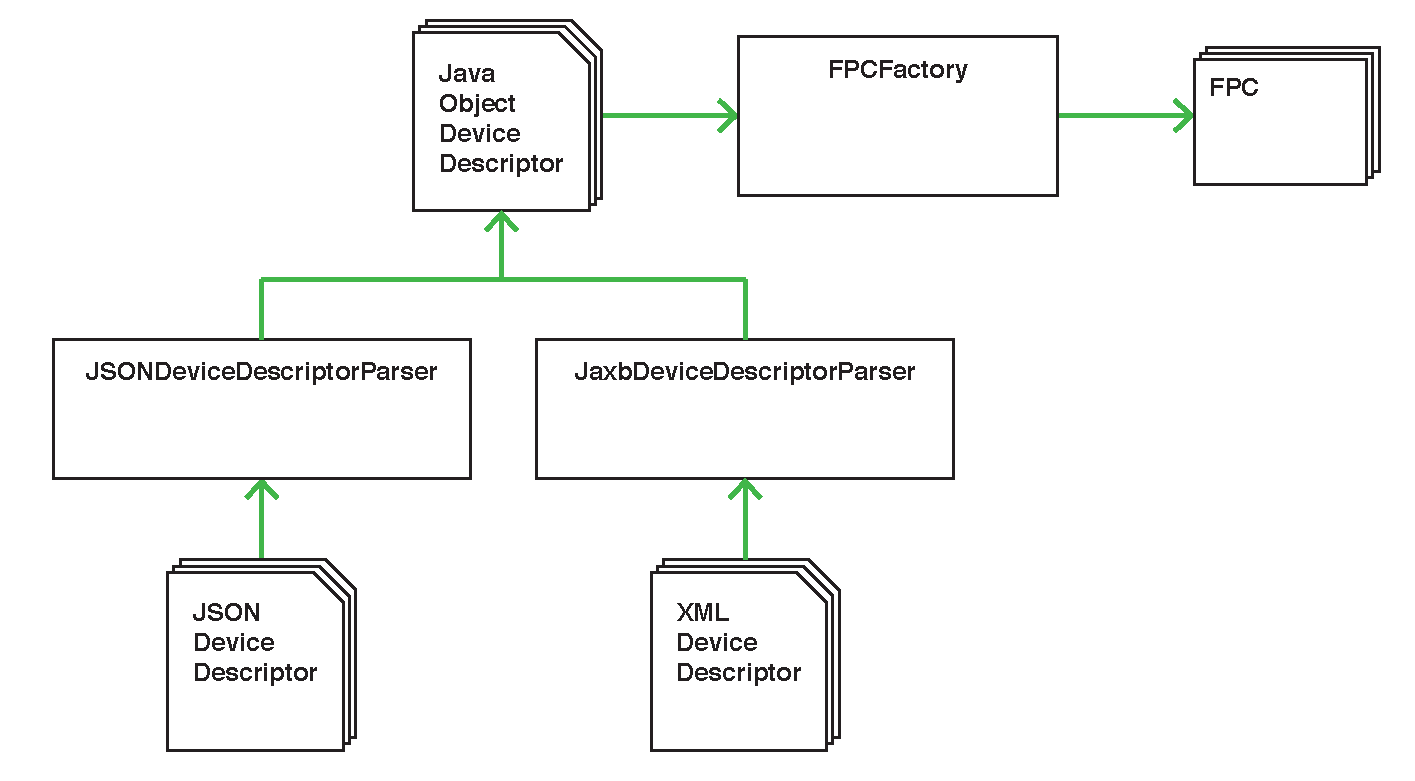
\includegraphics[width=\textwidth]{imgs/descriptorparser.pdf}
    \caption{Translation of different Device Descriptor formats into an
    intermediary Java representation}
    \label{fig:descriptorparser}
\end{figure}


Figure~\ref{fig:descriptorparser} shows a section of a hypothetical Middleware
setup. As can be seen, Device Descriptors are parsed and transliterated into
an intermediate Java representation before being handed over to the
\texttt{FPCFactory}. This decoupling process, performed by the
\texttt{DeviceDescriptorParser} interface, ensures that the \texttt{FPCFactory}
is not directly tied to any particular Device Descriptor format; as a result,
the introduction of a new descriptor syntax does not entail any change to the
\texttt{FPCFactory} itself, but only the creation of an approriate
\texttt{DeviceDescriptorParser} class. At the present moment, the PerLa
Middleware includes a \texttt{JaxbDeviceDescriptParser} implementation, which
is responsible for translating the XML Device Descriptor syntax shown in
previous sections of this document into the corresponding
\texttt{DeviceDescriptor} Java class required by the \texttt{FPCFactory}.

~\\
\lstset{language=java}
\begin{lstlisting}[caption={The DeviceDescriptorParser interface. The only
method exposed by this module is responsible for converting Device Descriptors
received from the sensing nodes into an intermediate Java object
representation.}]
public interface DeviceDescriptorParser {
    public DeviceDescriptor parse(InputStream is)
            throws DeviceDescriptorParseException;
}
\end{lstlisting}

The \texttt{FPCFactory}, in its essence, is a coordinator object that delegates
the actual construction of all \texttt{FPC} components to the various factory
modules described in the former sections of this chapter. This feature is an
essential characteristics of the new Middleware architecture, and constitutes
the basic building block of the PerLa pluggable module system. New
\texttt{Channels}, \texttt{IORequests}, and \texttt{Messages} can be added
simply by means of the \texttt{FPCFactory} constructor method (see
listing~\ref{lst:fpcfactory}), and don't require any modification to the
existing Middleware code; PerLa is open for extension but closed for
modification.

In addition to the creation of all \texttt{FPC} component modules, the
\texttt{FPCFactory} performs the following tasks:

\begin{itemize}

    \item Parses the \lstinline!<operation>! Device Descriptor section and
        compiles all PerLa \texttt{Scripts} in their intermediate SIR form;

    \item Associates every declared device \texttt{Attribute} to the
        \texttt{Operation} that is responsible for its management;

    \item Assembles the various component modules, \texttt{Operations} and
        \texttt{Scripts} inside a single \texttt{FPC} object.

\end{itemize}

~\\
\lstset{language=java}
\begin{lstlisting}[caption={The FPCFactory class methods},label={lst:fpcfactory}]
public class FPCFactory { 
   public BaseFpcFactory(List<MapperFactory> mapperFactoryList,
            List<ChannelFactory> channelFactoryList,
            List<IORequestBuilderFactory> requestBuilderFactoryList)
    
    public Fpc createFpc(DeviceDescriptor descriptor, int id)
            throws InvalidDeviceDescriptorException;
}
\end{lstlisting}


\subsection{Registry}

The \texttt{Registry} is a simple in-memory database that stores \texttt{FPC}
objects. It is primarily employed for the discovery of sensing devices
registered in a running PerLa instance, and its services are extensively
exploited by the Query Executor component for the management of \texttt{EXECUTE
IF} statements. Its interface, available in listing~\ref{lst:registry}, is
straightforward and easy to use. It is composed of two data manipulation
methods, namely \texttt{add()} and \texttt{remove()}, and three data retrieval
methods, \texttt{get()}, \texttt{getAll()} and \texttt{getByAttribute}.

\texttt{add()} and \texttt{remove()} allow PerLa users to respectively insert
and delete \texttt{FPC} objects from the \texttt{Registry}. The first method is
primarily used by the \texttt{FPCFactory}, which is responsible for registering
newly connected devices, whereas the second is invoked from the \texttt{FPC}
itself when the controlled node stops operating.

The data retrieval section of the \texttt{Registry} interface comprises three
methods with different semantics. \texttt{get()} can be used to retrieve a
single \texttt{FPC} object with a specific identifier, and is usually invoked
when the user needs to address a certain device in a Pervasive Network.
\texttt{getAll()} is a shortcut that returns a list with all the \texttt{FPC}
objects connected to PerLa. The last method, \texttt{getByAttribute()}, allows
PerLa users to select a subset of devices with well-defined characteristics;
its two parameters can in fact be used to indicate the precise set of data
\texttt{Attributes} that a remote node must possess in order to be considered
in the selection.

~\\
\lstset{language=java}
\begin{lstlisting}[caption={The Registry interface},label={lst:registry}]
public interface Registry {
    public Fpc get(int id);
    
    public Collection<Fpc> getAll();

    public Collection<Fpc> getByAttribute(Collection<Attribute> with,
        Collection<Attribute> without);
    
    public void add(Fpc fpc);
    
    public void remove(Fpc fpc);
}
\end{lstlisting}



		\chapter{Conclusions}
\label{cha:conclusions}

This thesis described the design and implementation of an asynchronous data
access middleware for Pervasive Systems. As shown in previous chapters, this
process began with an analysis aimed at identifying the weaknesses and
strengths of the Classic PerLa Middleware architecture, which was later used to
outline a basic set of goals to be followed during the development of the
software hereby described. From these goals ensued a New Middleware design
(chapter~\ref{cha:middleware_overview}), and a concrete implementation
(chapter~\ref{cha:components}). The most important contributions that the
development of this new data access middleware brought to the PerLa System can
be classified into three categories: modularization of the Plug \& Play device
registration process, asynchronous data flow management, and an improved
\texttt{FPC}. 

The new Plug \& Play device registration process was enhanced with three
distinct measures: first, the internal structure of the \texttt{FPC} component
was split into independent modules; second, the \texttt{FPCFactory} itself was
partitioned into several sub-factory units, one for each \texttt{FPC} module;
third, a Plugin System was designed to allow the addition of new \texttt{FPC}
fragments without requiring any direct modification to the \texttt{FPCFactory}
itself. The advantages and merits of this new modular design were tested and
validated with the implementation of five different modules, three created by
the author of this thesis (\texttt{JSONMapper}, \texttt{URLEncodedMapper} and
\texttt{SimulatorChannel}), and two by other graduate student
(\texttt{HTTPChannel} and \texttt{TinyOSChannel}).

Another crucial aspect of the New PerLa Middleware design is represented by the
asynchronous data flow management paradigm. As explained in
section~\ref{sec:newmiddleware.async}, all components of the new architecture
implement an asynchronous event-driven API that improves both memory usage and
global reaction times of the entire system. An example of the benefits brought
by this new paradigm can be derived by analysing the number of threads
instantiated for each \texttt{FPC}. In the Classic Middleware, each
\texttt{FPC} was composed of four distinct Java threads: one dedicated to
reading incoming messages, one for the \texttt{Unmarshaller}, one for the
\texttt{Marshaller}, and one for the creation of output records. Conversely,
within the New Middleware infrastructure, a single Java thread located in the
\texttt{Channel} module is enough to drive all data handoffs occurring inside
an entire \texttt{FPC}. Although additional threads may be instantiated during
the execution of PerLa \texttt{Script}s, it is worth noting that these are
managed by the \texttt{Script Engine}, and are always shared among all running
\texttt{FPC}s; as a consequence, the New Middleware can dynamically adjust its
resource consumption figures to match the actual workload (see
chapter~\ref{cha:components} for additional details).

The \texttt{FPC} benefits from another improvement brought by the New
Middleware design, namely the PerLa Scripting Language. This new feature
complements the declarative nature of the Device Descriptor, enabling the
definition of advanced mappings between device capabilities and data
\texttt{Attributes} exposed by the \texttt{FPC} component. The imperative
programming paradigm fostered by the PerLa Scripting Language proved to be a
key addition to the Middleware architecture, as it enhanced the flexibility and
versatility of the entire PerLa System; \texttt{Script}s have in fact been used
to define complex device initialization procedures, to aggregate the
information collected from a sensing network, and to reshape the contents of
hierarchical data structures into the one-dimensional record pattern produced
by the \texttt{FPC} component. It is in the author's view that the former
Device Descriptor structure could not be used to adequately model the
aforementioned applications, as its inherently declarative essence embodied a
fixed set of behavioural assumption which were forced on all nodes of the
Pervasive Network.  The PerLa Scripting Language proposes itself as a less
opinionated tool that can be used by node developers to better specify the
functioning mechanisms of their devices.


\section{Future work}

\subsection{Implementation of new plugins}

The New PerLa Middleware is designed to be extended through the addition of new
modules, and it should come as no surprise that one of its intended evolution
paths consists in fact in the development of new Plugins. As described in
chapter~\ref{cha:components}, there are two main types of modules that can be
added to the PerLa Plugin System: \texttt{Channels} and \texttt{Mappers}.

The possibility to add new \texttt{Channel} implementations is a distinguishing
feature of the New Middleware design that should be effectively exploited to
expand the range of supported endpoint devices. At the time of writing the
selection of Plugins shipped with the core Middleware distribution allows PerLa
to connect with HTTP services and TinyOS motes. This initial line-up should be
only considered as a starting point, since a larger assortment of communication
systems is required to manage even the most rudimentary Pervasive System. The
following list contains a choice of protocols and networking technologies for
which a dedicated \texttt{Channel} implementation is advised:

\begin{itemize}

    \item \textbf{TCP/IP:} Widely employed in a vast variety of devices,
    ranging from high-end personal computers to low power devices;

\item \textbf{Bluetooth LE (Low Energy):} One of the leading technologies for
    wireless personal area networks. Currently supported by all major operating
    systems, Bluetooth LE found its way into many devices and appliances, like
    fitness bands, smartphones, healthcare instruments, home entertainment sets
    and localization beacons;

    \item \textbf{IEEE 802.15.4 based protocols:} IEEE 802.15.4 is a physical
    layer widely employed in many personal area network protocols. It is the
    foundation of several networking specifications like Zigbee, Xbee and MiWi;

    \item \textbf{RS232:} Serial port communication. Its implementation should
    be considered in order to connect with legacy devices and other low power
    systems (e.g., Arduino).

\end{itemize}

\texttt{Mapper}s represent another extension point of the PerLa Middleware
infrastructure that can be used to manage additional data formats and
encodings. The only \texttt{Mapper} components available as of December 2014 in
the core Middleware distribution provide support for JSON and URL-encoded data
structures. Analogously to what already stated for the \texttt{Channel}
component, future PerLa developers should consider implementing new
\texttt{Mapper}s for handling the following data formats:

\begin{itemize}

    \item \textbf{C/C++ structs:} Its implementation should be a simple
    backport from the Classic Middleware architecture;

    \item \textbf{XML:} A markup language for document encoding;

    \item \textbf{CSV (Comma-Separated Values):} A simple format for the
    transmission and storage of tabular data.

\end{itemize}

\subsection{Alternative Device Descriptor forms}

As introduced in chapter~\ref{cha:components}, the new Plug \& Play node
registration system is comprised of two separate elements: a
\texttt{DeviceDescriptorParser} front-end, which analyzes the Device Descriptor
to build a format-agnostic Java representation of the descriptor itself, and
the \texttt{FPCFactory}, which consumes this intermediate Java representation
to assemble the final \texttt{FPC}. This new architecture was conceived to
facilitate the future addition of alternative Device Descriptor formats by only
requiring the development of an appropriate \texttt{DeviceDescriptorParser}
module.

There are two main reasons for adding a new Device Descriptor representation:
first, to support a different data format that may be more convenient for some
devices (e.g., a JSON Device Descriptor); second, to create \texttt{FPC}s using
readily available industry standard device description technologies. This
former motivation leads us to one future development of the PerLa
infrastructure, namely the possibility of introducing a
\texttt{DeviceDescriptorParser} for the \textit{SensorML} \cite{sensorml}
sensor description format. Through this effort the PerLa Middleware would be
immediately compatible with all devices for which a SensorML description is
already available.

\subsection{Distributed PerLa}

Future development of the PerLa Middleware should aim at implementing
in-network processing capabilities in order to better exploit the resources
available in a Pervasive System. Such efforts must focus on the definition of a
software distribution infrastructure that can be used to divide a high-level
computation into smaller, independent units of work to be executed on the
individual nodes of the sensing network.

		\chapter{In-depth component description}

\section{Communicating with Channels}
\label{sec:channel}

\texttt{Channel} is an interface for performing I/O operations. It represents
the principal abstraction used by the middleware to communicate with hardware
devices and external software services.

\lstset{language=Java}
\begin{lstlisting}[float,caption=The Channel interface,label={lst:channel}]
public interface Channel {

	public String getId();
	
	public IOTask submit(IORequest request, IOHandler handler)
			throws ChannelException;
	
	public void setAsyncIOHandler(IOHandler handler)
			throws IllegalStateException;
			
	public boolean isClosed();
	
	public void close();
			
}
\end{lstlisting}

The \texttt{Channel} interface is not tied to any specific technology or
communication stack; as a result of this design choice, a wide variety of data
management tasks, including but not limited to, networking, file handling, and
automatic data generation can be implemented as \texttt{Channel}s.

The current Middleware architecture encourages the creation of several highly
specialized \texttt{Channel}s, which are usually developed around third-party
communication libraries. \texttt{HTTPChannel}, a \texttt{Channel} providing
support for HTTP communications, is an excellent example of the advantages of
this design strategy. Implemented as a simple wrapper around Apache's HTTP
Components toolkit, its development only required a basic understanding of the
HTTP protocol; yet \texttt{HTTPChannel} is a fully compliant HTTP/1.1 client
(see section~\ref{sec:channel.implementations} for additional details).

Upon instantiation, \texttt{Channel}s are open and ready to be used. They may
be optionally closed to relinquish unused resources by invoking the
\texttt{close()} method. Once closed, a \texttt{Channel} cannot be re-opened,
and every subsequent attempt to perform an I/O operation will fail causing a
\texttt{ChannelException} to be thrown. The current state of a \texttt{Channel}
can be probed through its \texttt{isClosed()} method.

Bytes sent or received with a \texttt{Channel} are encapsulated in a
\texttt{Payload} object. As shown in listing~\ref{lst:payload}, the
\texttt{Payload} interface allows all Middleware components to handle different
data types with a common set of methods, regardless of their individual
encoding.  \texttt{Payload}s will be the subject of further discussion in
section~\ref{sec:components.mapper}

\lstset{language=Java}
\begin{lstlisting}[float,caption=The Payload interface,label={lst:payload}]
public interface Payload {

	public Charset getCharset();

	public InputStream asInputStream();

	public ByteBuffer asByteBuffer();

	public String asString();

}
\end{lstlisting}

All user-initiated I/O operations begin with an invocation of the
\texttt{Channel.submit()} method. As can be seen in listing~\ref{lst:channel},
\texttt{submit()} is a direct implementation of the asynchronous interaction
paradigm introduced in section~\ref{sec:newmiddleware.async}. The emphasis on
asynchronous execution is underscored by the absence of blocking operations in
the \texttt{Channel} interface. This aspect is of paramount importance for the
entire Middleware design, as implementing a truly asynchronous system would
prove impossible if such feature were not provided by its core data access
layer.


\subsection{Instantiating new Channels}

\texttt{Channel}s are created by means of the \texttt{ChannelFactory}
interface, a reification of the Factory design pattern that allows polymorphic
instantiation of new object classes.

By using a Factory instantiation model, the choice of a particular
\texttt{Channel} implementation can be postponed from compile time to run time.
This technique allows the Middleware to dynamically adapt in response to
environment changes, and to support extension through the addition of new
user-defined \texttt{Channel}s. For further information regarding the Factory
pattern and its other uses inside the PerLa Middleware, refer to
section~\ref{sec:newmiddleware.factory}.

All the information required to create a new \texttt{Channel} is stored inside
a \texttt{ChannelDescriptor}. As shown in listing~\ref{lst:channelFactory},
this configuration object is the only parameter required to correctly invoke
the \texttt{createChannel()} method.

\lstset{language=Java}
\begin{lstlisting}[float,caption=The ChannelFactory
interface,label={lst:channelFactory}]
public interface ChannelFactory {

	public Class<? extends ChannelDescriptor>
			acceptedChannelDescriptorClass();

	public Channel createChannel(ChannelDescriptor descriptor)
			throws InvalidDeviceDescriptorException;

}
\end{lstlisting}

\begin{figure}[h!]
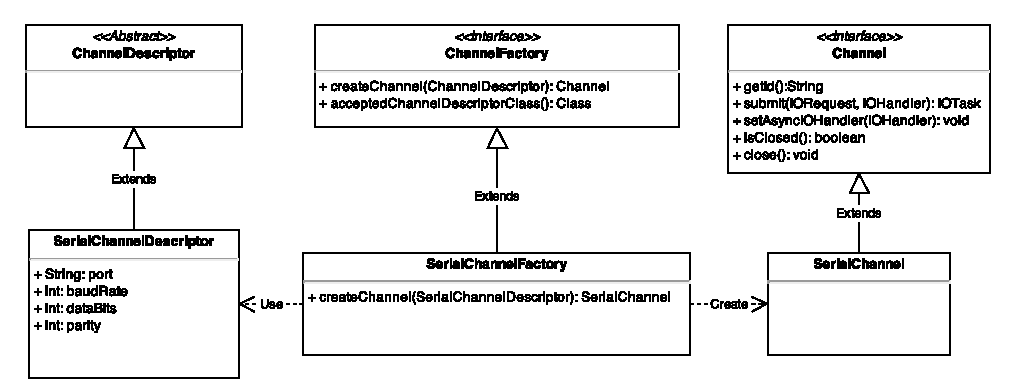
\includegraphics[width=\textwidth]{imgs/channel_factory.pdf}
\caption{Class diagram of the Channel layer}
\end{figure}

Each \texttt{ChannelFactory} is tied to a specific communication technology;
therefore, it can only accept a single class of \texttt{ChannelDescriptor}
objects. For example, the \texttt{HTTPChannelFactory} parses
\texttt{HTTPChannelDescriptor}s and creates \texttt{HTTPChannel}s, whereas an
hypothetical \texttt{SerialChannelFactory} would consume
\texttt{SerialChannelDescriptor}s to create \texttt{SerialChannel}s. Failure to
provide a suitable \texttt{ChannelDescriptor} object will cause the
\texttt{createChannel()} method to throw an
\texttt{InvalidDeviceDescriptorException}.

The \texttt{acceptedChannelDescriptorClass()} method can be used to dynamically
discover which \texttt{ChannelDescriptor} type is supported by a specific
\texttt{ChannelFactory}. This method is the fulcrum of the \texttt{Channel}
Plugin System, as it allows the Middleware to invoke the most appropriate
\texttt{ChannelFactory} using only information available at runtime.

\begin{figure}[!hbt]
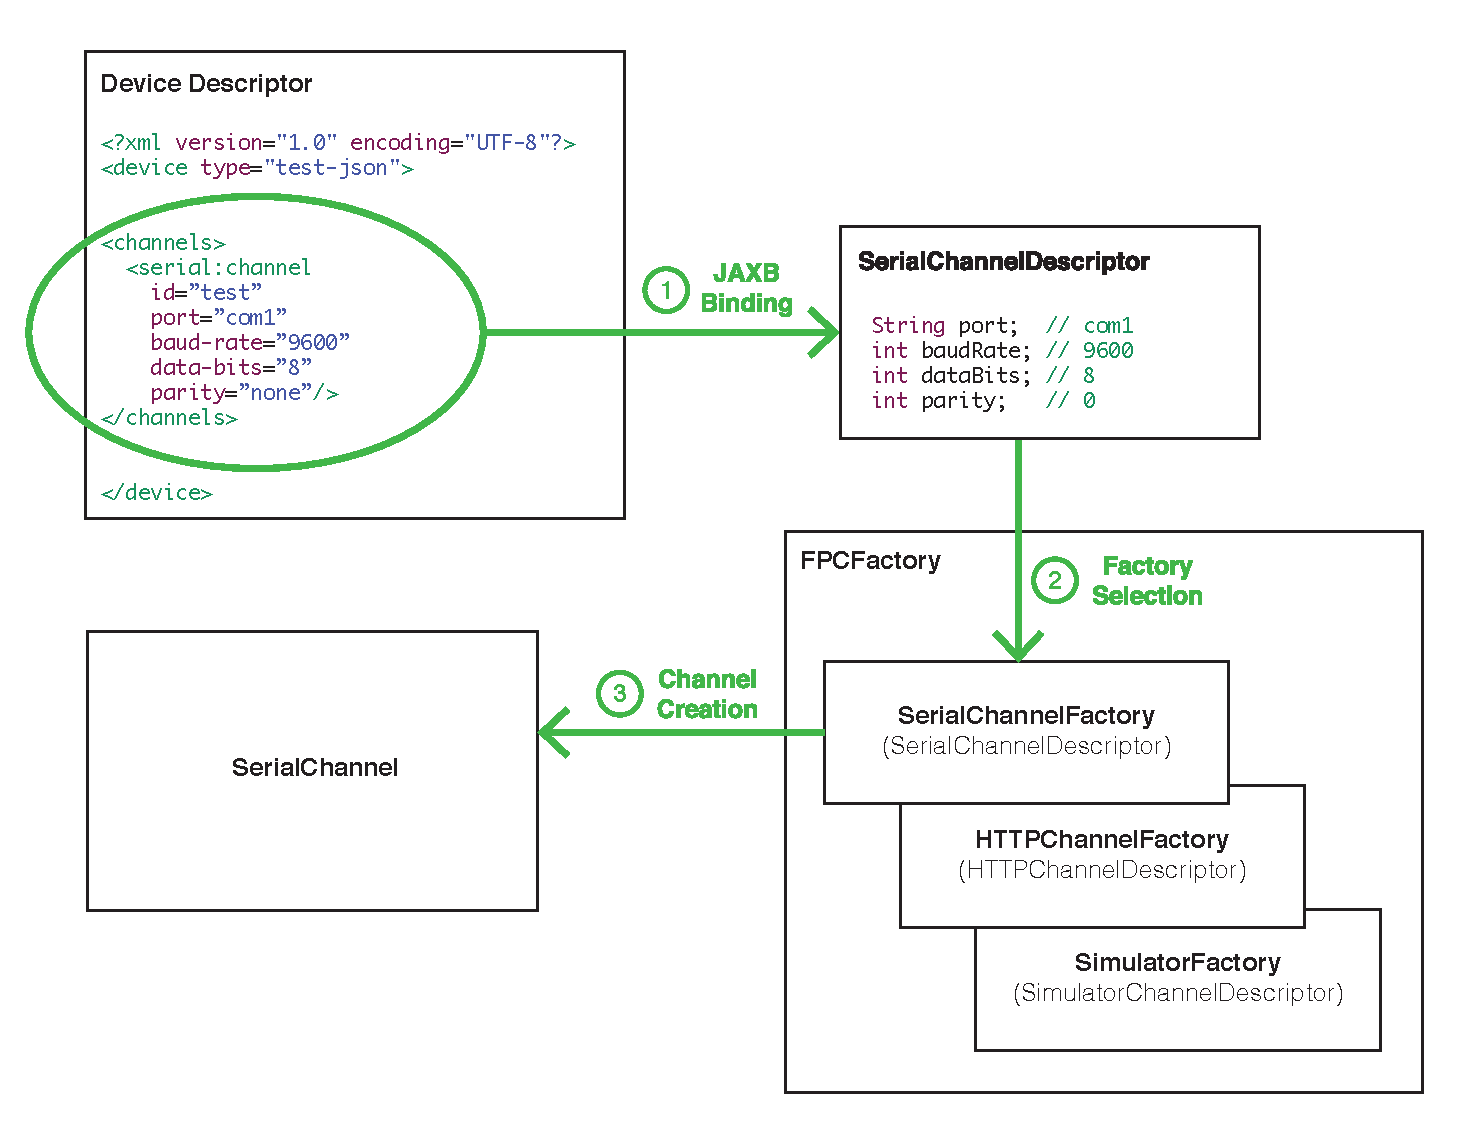
\includegraphics[width=\textwidth]{imgs/channel_creation_process.pdf}
\caption{The Channel creation process}
\label{fig:channel.creation}
{
\begin{figurenote}
This figure illustrates the \texttt{Channel} creation process executed by the
Middleware upon reception of a new Device Descriptor.  \begin{enumerate}
  \itemsep0em
  \item JAXB binds the XML Device Descriptor to an apropriate
\texttt{ChannelDescriptor} object using namespace information \item A suitable
\texttt{ChannelFactory} is selected at runtime using the
\texttt{acceptedChannelDescriptorClass()} method
  \item The information contained in the \texttt{SerialChannelDescriptor} is
used to create a new \texttt{SerialChannel} \end{enumerate}
\end{figurenote}
}
\end{figure}

\texttt{ChannelDescriptor} objects are automatically created by the
Middleware using the information contained in the Device Descriptor XML files.
This binding process is performed by the JAXB library, which is also
responsible for instantiating the correct \texttt{ChannelDescriptor} class
using XML Namespace information. Figure~\ref{fig:channel.creation} illustrates
this technique, and ties it together with the other operations described in
this section.

It is important to note that a single JVM instance running the PerLa Middleware
may host several \texttt{Channel} objects of the same type, at the same time.
Several devices can use the same communication technology, and the
\texttt{ChannelFactory} may determine that it's best to create an individual
\texttt{Channel} for each one of them. This behaviour is fostered by the new
\texttt{ChannelFactory} architecture, and is considered idiomatic design;
hence, it would not be uncommon to implement the hypothetical
\texttt{SerialChannelFactory} introduced in the previous paragraphs so that
every serial port is handled by a different \texttt{SerialChannel} instance.


\subsection{IORequest management}

\texttt{IORequest} is the base object interface employed to interact with a
sensing node connected to the Middleware. It contains two types of information:
the payload to be transferred, and \texttt{Channel}-dependent data needed for a
correct communication with the endpoint device.

\lstset{language=Java}
\begin{lstlisting}[float,floatplacement=!hbt,caption=The IORequest
interface,label={lst:iorequest}]
public interface IORequest {

	public String getId();

	public void setParameter(String name, Payload payload);
	
}
\end{lstlisting}

Every \texttt{Channel} imlementation is bundled with its own custom
\texttt{IORequest} class. Following up on previous examples, the
\texttt{HTTPChannel} package contains a \texttt{HTTPIORequest} object, whereas
the fictitious \texttt{SerialChannel} would be supplied with a
\texttt{SerialIORequest} class of request objects. This additional level of
indirection is necessary since different communication technologies require
different settings to establish end-to-end connectivity; therefore, a universal
\texttt{IORequest} object would soon prove to be a limiting factor for the
extension of the Middleware.

As shown in listing~\ref{lst:iorequest}, payload data can be set in an
\texttt{IORequest} by means of the \texttt{setParameter()} method.
\texttt{Payload}s are addressed by name, and a single \texttt{IORequest}
implementation may support several at once. The exact set of \texttt{Payload}
parameters accepted by an \texttt{IORequest} class depends on the design of its
matching \texttt{Channel}; for example, the \texttt{HTTPChannel}
implementation supports three: an `entity' payload (request body), a `query'
payload (an URL-encoded string), and a `path' payload (a path component used to
identify a single resource accessible from the base URL).

\texttt{IORequest}s are disposable objects; they are created, submitted to a
\texttt{Channel}, and garbage collected once the communication is over.
Creation is performed by means of a factory interface dubbed
\texttt{IORequestBuilder}, which allows the Middleware to build new copies of
an \texttt{IORequest} from a fixed template. It is important to note that
request objects built using this technique do not contain \texttt{Payload}
parameters; these are to be added manually before subbmitting the
\texttt{IORequest} to a \texttt{Channel}.

Besides \texttt{IORequest} creation, the \texttt{IORequestBuilder} interface
can be used to dynamically discover which \texttt{Payload} parameters are
supported by an \texttt{IORequest}. This functionality, exposed through the
\texttt{getParameterList()} method, is a crucial component of the Middleware
Plugin System, as it allows \textit{Script} instructions to determine whether
an \texttt{IORequest} was populated with all the necessary \texttt{Payload}
parameters or not. This concept will be the subject of further analysis in
section~\ref{sec:components.script}.

A single device connected to the PerLa Middleware is generally managed using
several \texttt{IORequestBuilder}s, any one of which is responsible for
creating a request object suitable to control a single aspect of
the interaction with the endpoint. The main advantage brought by this
templating mechanism is that \texttt{Channel}-related configuration settings
are only specified once, hence the same \texttt{IORequest} structure can be
reused multiple times to transport different payload information.

\lstset{language=Java}
\begin{lstlisting}[float,floatplacement=!hbt,caption=The IORequestBuilder
interface,label={lst:iorequestbuilder}]
public interface IORequestBuilder {

	public String getRequestId();

	public IORequest create();

	public abstract List<IORequestParameter> getParameterList();

	public static class IORequestParameter {

		public String getName() {
			return name;
		}

		public boolean isMandatory() {
			return mandatory;
		}

	}
}
\end{lstlisting}

REST APIs are an excellent use case to demonstrate the aforementioned concept,
as every operation on a RESTful resource can be easily abstracted using an
appropriately configured request builder. By using
\texttt{HTTPIORequestBuilder} objects, HTTP protocol information (base URL,
method, header, \ldots) are specified one single time only for
every REST endpoint. Once this step is done, the API can be invoked just by
building new \texttt{IORequest}s and submitting them to a \texttt{HTTPChannel}.

\begin{figure}[!hbt]
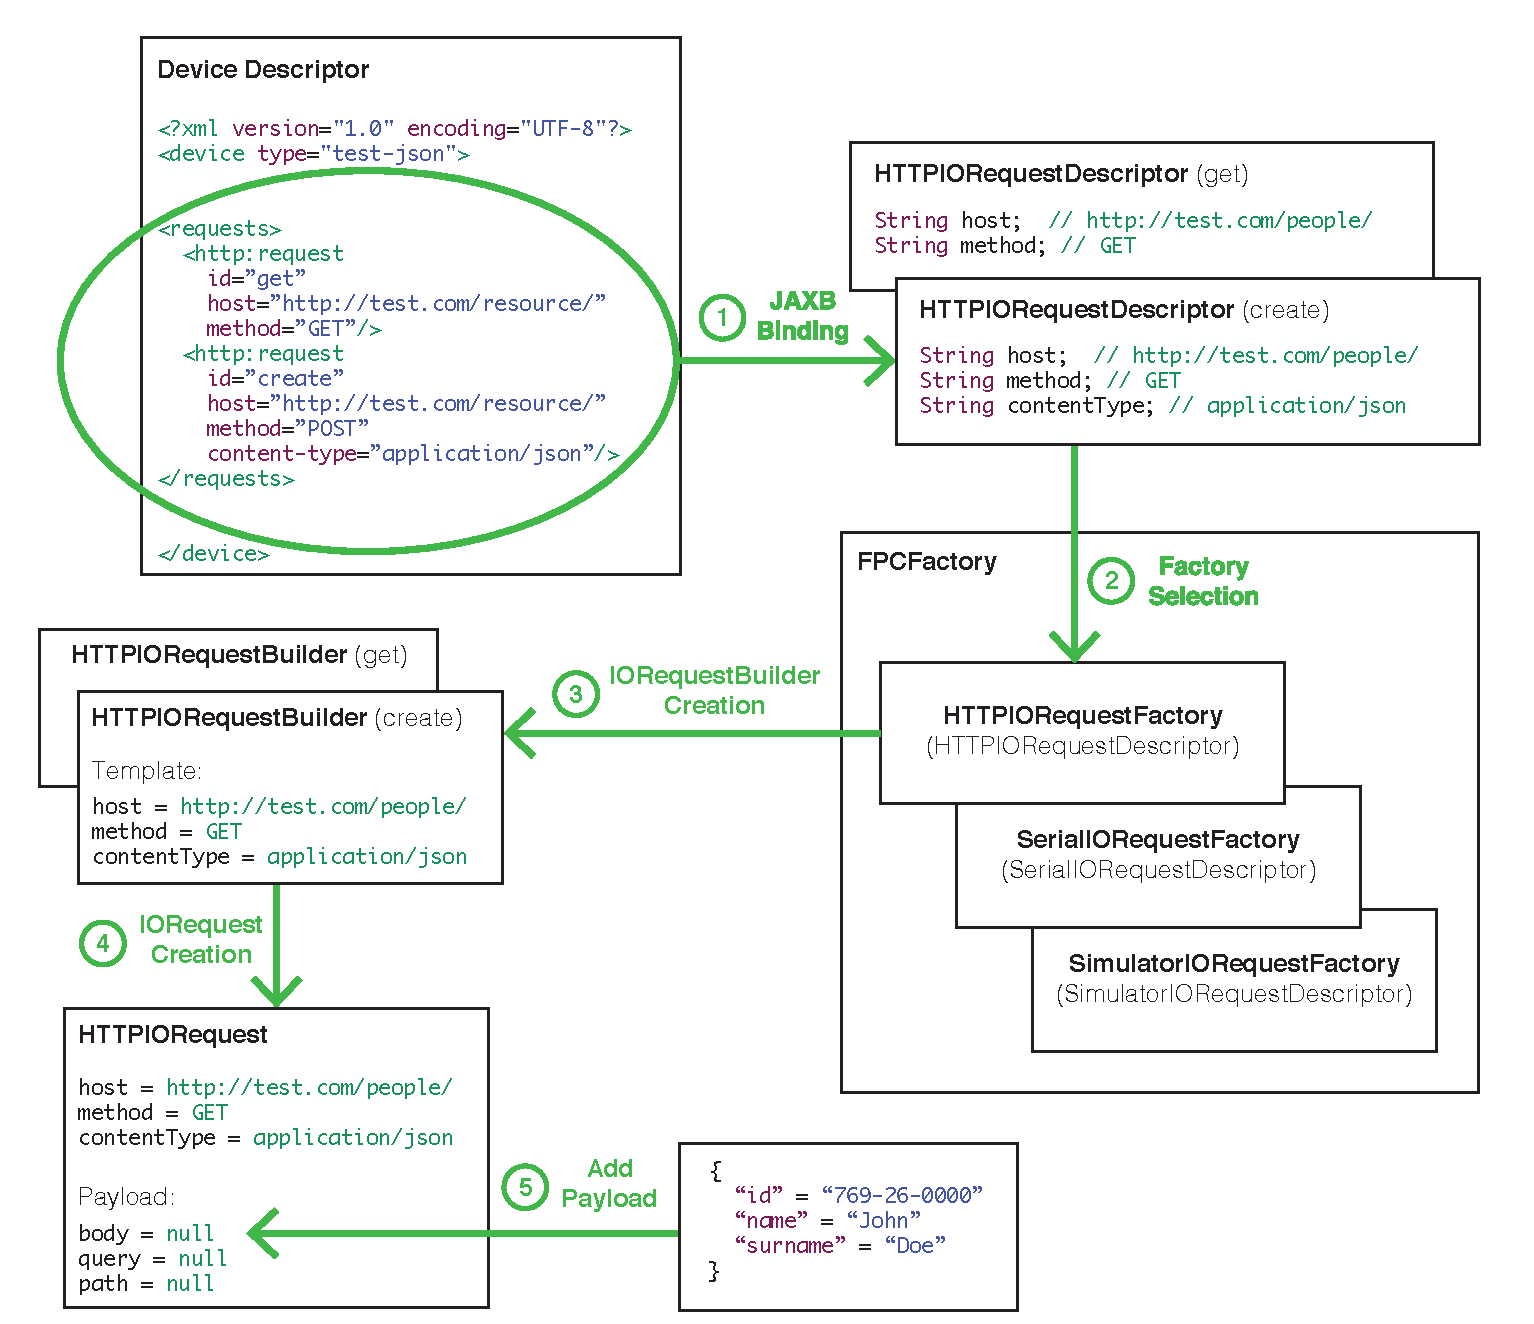
\includegraphics[width=\textwidth]{imgs/iorequest_creation_process.pdf}
\caption{The IORequest creation process}
\label{fig:iorequest.creation}
{
\begin{figurenote}
This figure illustrates the autonomous creation of \texttt{IORequest} objects.
Steps 1 to 3 are performed only once after receiving the Device Descriptor,
whereas steps 4 and 5 are repeated every time the REST API is to be invoked.
\begin{enumerate}
  \itemsep0em
  \item JAXB binds the XML Device Descriptor to an apropriate
\texttt{IORequestDescriptor} object using namespace information \item A
suitable \texttt{IORequestBuilderFactory} is selected at runtime using the
\texttt{acceptedIORequestDescriptorClass()} method
  \item The information contained in the \texttt{IORequestDescriptor} is used
to create a new \texttt{IORequestBuilder} \item The \texttt{IORequestBuilder}
is used to create new \texttt{IORequest} copies using the internal template
  \item The newly created \texttt{IORequest} objects can be populated with
\texttt{Payload} parameters as needed \end{enumerate}
\end{figurenote}
}
\end{figure}

\texttt{IORequestBuilder}s are created by means of an
\texttt{IORequestBuilderFactory}, an object that implements the now familiar
Factory design pattern. Creation proceeds as follows: the request template is
loaded from an XML Device Descriptor, bound to an appropriate
\texttt{IORequestDescriptor}, and processed by the
\texttt{IORequestBuilderFactory} to create the corresponding
\texttt{IORequestBuilder}. Similarly to what already seen in the previous
section, every \texttt{IORequestBuilderFactory} implements an
\texttt{acceptedIORequestDescriptorClass()} method, which can be used to
dynamically determine if a factory object can parse a specific type of
\texttt{IORequestDescriptor}. It should come as no surprise that every
\texttt{IORequestBuilder} class is provided with complementary
\texttt{IORequestBuilderFactory} and \texttt{IORequestDescriptor}
implementations.

\begin{figure}[!hbt]
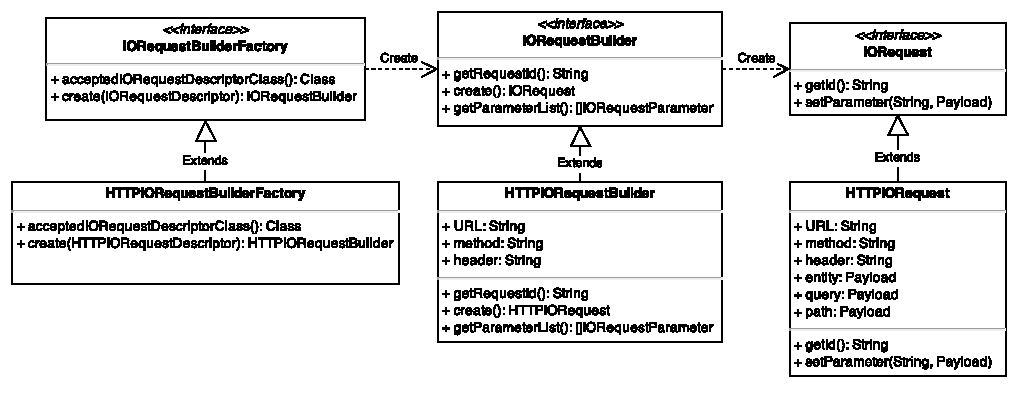
\includegraphics[width=\textwidth]{imgs/iorequest.pdf}
\caption{The extended IORequest class diagram. For additional information about
the IORequestParameter object consult listing 1.5.} \label{fig:iorequest.class}
\end{figure}


\subsection{Handling asynchronous I/O operations}

As mentioned in previous sections, communication with a device connected to the
PerLa Middleware is achieved by means of the \texttt{Channel.submit()} method.
Invocations of \texttt{submit()} are non-blocking; control flow is immediately
returned to the caller, thus allowing other computations to be performed while
the requested I/O operation is being processed.

As can be seen in listing~\ref{lst:channel}, \texttt{submit()} requires two
parameters: an \texttt{IORequest} and an \texttt{IOHandler} callback object.
The former specifies which I/O operation is to be performed, while the latter
allows the caller to be asynchronously notified of its completion.

The \texttt{IOHandler} interface is composed of two methods, namely
\texttt{complete()} and \texttt{error()}, which are invoked when processing of
an I/O operation comes to an end. It is important to note that both these
methods always carry context information in the form of an \texttt{IORequest},
which is guaranteed to be the same exact object used for starting the I/O
operation whose completion is being notified. For this reason,
\texttt{IOHandler} can be considered the nexus of the asynchronous invocation
model, as it connects \texttt{IORequest} objects with the outcome of the
corresponding I/O operation performed by the \texttt{Channel}.

\lstset{language=Java}
\begin{lstlisting}[float,floatplacement=H,caption=The IOHandler
interface,label={lst:iohandler}]
public interface IOHandler {
	public void complete(IORequest request, Optional<Payload> result);
	
	public void error(IORequest request, Throwable cause);
}
\end{lstlisting}

\lstset{language=Java}
\begin{lstlisting}[float,floatplacement=!hbt,caption=The IOTask
interface,label={lst:iotask}]
public interface IOTask {
	public void cancel();
	
	public IORequest getRequest();
	
	public boolean isCancelled();
	
	public boolean isDone();
}
\end{lstlisting}

Semantically, an invocation of the \texttt{complete()} method is always
associated with the successful termination of an I/O operation. As shown in
listing~\ref{lst:iohandler}, this method includes an optional \texttt{Payload}
object, that contains all data received from the endpoint device. A call to
\texttt{complete()} with an empty \texttt{Payload} indicates that the I/O
operation was completed without errors, but no data was received. Conversely,
an invocation of the \texttt{error()} method indicates that the I/O operation
was aborted before completion. In this case the cause of failure is always
notified through the \texttt{cause} parameter.

From the point of view the Java memory model, the \texttt{Channel.submit()}
creates a happens-before relationship with \texttt{IOHandler.complete()} and
\texttt{IOHandler.error()}, viz. any side effect generated by the code that led
to the \texttt{submit()} invocation is guaranteed to be visible in the
\texttt{complete()} and \texttt{error()} callback methods.

Asynchrous execution does not imply loss of control; ongoing I/O operations can
be monitored or cancelled by means of the \texttt{IOTask} object acquired upon
submitting an \texttt{IORequest}. Listing~\ref{lst:iotask} shows all methods of
the \texttt{IOTask} interface; method names are self explanatory, and the
reader should be able to deduce their purpose just by analyzing their 
signature. The only nuance worth mentioning is that
\texttt{isCancelled()} always implies \texttt{isDone()} (i.e., all cancelled
I/O operations are also complete), while the opposite does not hold (i.e., not
all complete I/O operations were cancelled).

\begin{figure}[!hbt]
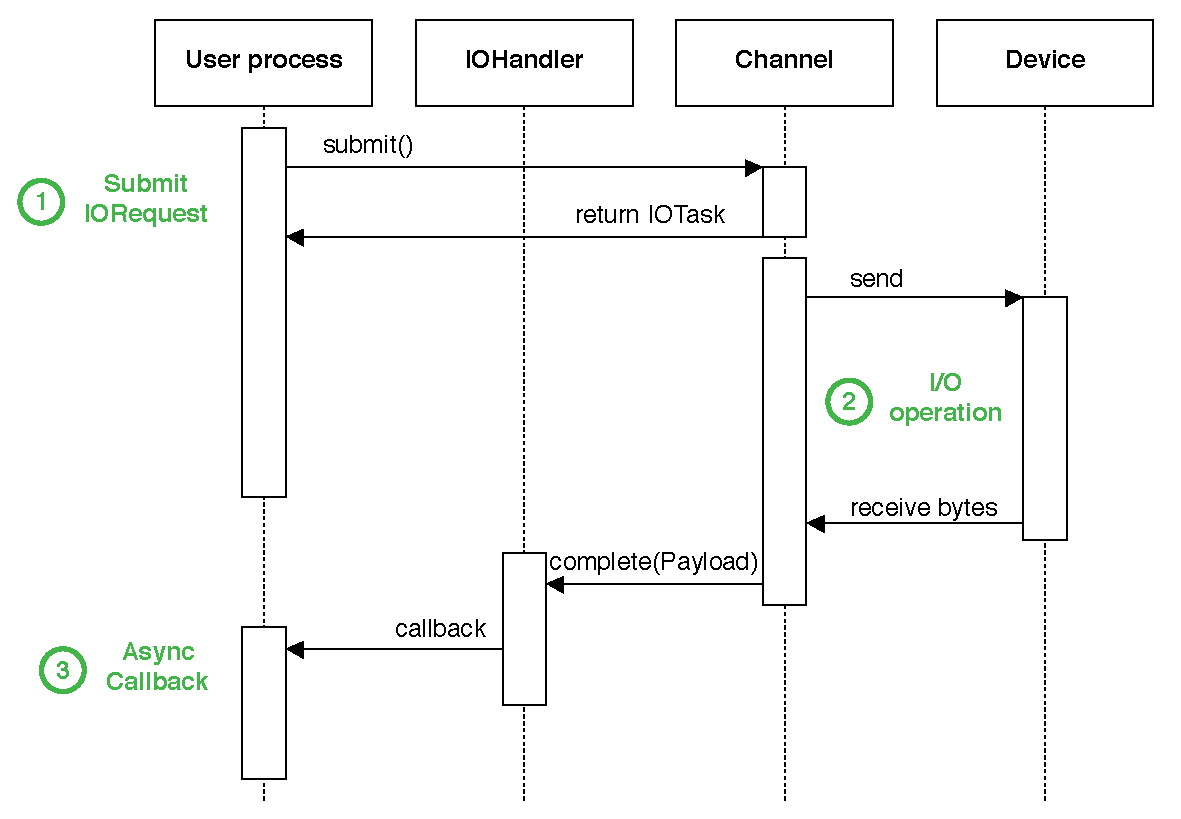
\includegraphics[width=\textwidth]{imgs/async_channel_sequence.pdf}
\caption{Sequence diagram of an asynchronous I/O operation. Note that the user
process and the I/O operation are executed in parallel.}
\label{fig:channel.async}
\end{figure}

The \texttt{Channel} interface is also designed to manage completely
asynchronous I/O operations, namely communication efforts spontaneously
initiated by the remote device. This communication model is popular among WSNs,
as it is often employed to handle periodic data streams or events happening
at irregular intervals. Such I/O operations can be handled through a catch-all
\texttt{IOHandler} set with the \texttt{setAsyncIOHandler()} method
(listing~\ref{lst:channel}). Since the communication is not initiated by the
Middleware, the \texttt{complete()} and \texttt{error()} callback methods will
be invoked with the \texttt{IORequest} parameter set to \texttt{null}.


\section{Handling data}
\label{sec:components.mapper}

\texttt{Payload} is a container for raw sequences of bytes. In spite of its
semplicity, this class forms the foundation of the entire PerLa Middleware, as
it is the vessel that conveys all information passing through the
\texttt{Channel} interface.

The data encapsulated in a \texttt{Payload} object is accessed one byte at a
time; this granularity level is ideal for the implemention of an I/O access
layer, whose sole concern consists in the transmission of information between
two endpoints, but is not suited to other forms of data management. Processing
the information contained in a \texttt{Payload} can be unwieldy and
unnecessarily complex; the byte-oriented interface doesn't provide any facility
for leveraging the underlying structure of the enclosed data, and even a simple
action like retrieving a value in a complex data structure can easily become a
daunting task.


\subsection{The Message interface}

\texttt{Message}s are structured data containers that enclose a group of
individual items called fields. The chief advantage that this data structure
provides over the simpler \texttt{Payload} object consists in the possibility
of addressing information by field name, a convenient feature that dispenses
with the burden of managing data in byte-sized chunks. The methods available in
the \texttt{Message} interface are shown in listing~\ref{lst:message}.

\lstset{language=Java}
\begin{lstlisting}[float,floatplacement=!hbt,caption=The Message
interface,label={lst:message}]
public interface Message {

    public String getType();

    public boolean hasField(String name);

    public Object getField(String name)
                throws IllegalArgumentException;

    public void setField(String name, Object value)
                throws IllegalArgumentException;

    public void appendElement(String name,Object element)
                throws IllegalArgumentException;

    public boolean validate();

}
\end{lstlisting}

The specific structure of a \texttt{Message} is defined by its type, which can
be queried through the \texttt{getType()} method. This property unequivocally
identifies the set of fields contained in a \texttt{Message} in terms of field
\textbf{name}, field \textbf{type} and field \textbf{qualifier}.

The field \textbf{name} is a textual attribute that uniquely identifies one
specific data item in the scope of a single \texttt{Message}. It can be used to
retrieve or set the value of a field through the \texttt{getField()} and
\texttt{setField()} methods respectively.

The \textbf{type} attribute defines the set of legal values that can be stored
in a field, together with the operations that are allowed on those values. It
is worth mentioning that this information is used to statically verify the type
safety of nearly all data management operations performed on a \texttt{Message}
(consult section~\ref{sec:components.script} for additional information). The
PerLa Middleware currently supports six primitive types:

\begin{itemize}

  \item \textbf{INTEGER}: a 32 bit signed two's complement integral data type

  \item \textbf{FLOAT}: a single-precision 32 bit IEEE 745 floating point

  \item \textbf{BOOLEAN}: a type with only two values, true or false

  \item \textbf{STRING}: a string of characters with UTF-16 encoding

  \item \textbf{TIMESTAMP}: a date with timezone, currently implemented using
      Java's \texttt{ZonedDateTime} class.

  \item \textbf{ID}: a unique label that identifies a single node connected in
      a PerLa managed network. The current implementation uses a 32 bit
      integer. 

\end{itemize}

Besides the data types presented above, fields can also be configured to hold
nested \texttt{Message}s. In this case, the type attribute must be set to the
particular type of \texttt{Message} that is to be stored in the field. 

The \textbf{qualifier} attribute is employed to define additional field
properties. It can be set to one of the following values:

\begin{itemize}

  \item \textbf{SIMPLE}: a normal field whose value can be altered and
      retrieved using the \texttt{setField()} and \texttt{getField()} methods
      respectively.

  \item \textbf{LIST}: a field that can hold multiple elements of the same
      type. New values can be added with the \texttt{appendElement()} method,
      and the entire list can be retrieved through the conventional
      \texttt{getField()} method. List-qualified fields preserve the order of
      insertion of the individual elements.

  \item \textbf{STATIC}: a field whose value is statically set when the
      \texttt{Message} type is declared. Any attempt to modify a
      statically-qualified field with either the \texttt{setField()} or the
      \texttt{appendElement()} methods will cause an exception to be thrown. It
      is important to note that static field values are set on a per-type
      basis; this means that all \texttt{Message}s of the same type will share
      the same field values for each static field (if any).
      
\end{itemize}


\subsection{Working with Messages: the Mapper interface}

\texttt{Message} objects are managed by the \texttt{Mapper} component. Its
interface, available in listing~\ref{lst:mapper}, groups all the
functionalities needed to handle a specific variety of structured information.
The one-to-one relationship between \texttt{Mapper}s and data types is
epitomized by the \texttt{getMessageType()} method, whose return value
indicates which \texttt{Message} class is supported by a particular
\texttt{Mapper}. This method is extensively employed by the Middleware to sift
through a collection of \texttt{Mapper}s, in order to find one that is best
suited for handling the information currently being processed.

\lstset{language=Java}
\begin{lstlisting}[float,floatplacement=!hbt,caption=The Mapper
interface,label={lst:mapper}]
public interface Mapper {

    public String getMessageType();

    public FieldDescriptor getFieldDescriptor(String name);

    public Collection<FieldDescriptor> getFieldDescriptors();

    public FpcMessage createMessage();

    public FpcMessage unmarshal(Payload payload);

    public Payload marshal(FpcMessage message);

}
\end{lstlisting}

Interactions with a \texttt{Mapper} usually begin with a call to the
\texttt{createMessage()} method, whose execution results in the creation of an
empty \texttt{Message} instance. Despite its unsuprising outcome, this method
draws once again our attention to the close relationship between
\texttt{Mapper}s and data types. Every \texttt{Mapper} instance is in fact
committed to the management of a precise class of information, hence all
\texttt{Message}s created with the \texttt{createMessage()} method will share
the same data type property, and, consequently, the same set of fields. The
interdependence between a \texttt{Mapper} and its assigned type is accentuated
even further by the \texttt{getFieldDescriptor()} and
\texttt{getFieldDescriptors()} methods, which can be used to analyze the
internal field structure characterizing all \texttt{Message} objects that the
\texttt{Mapper} creates. This introspective capability is extensively exploited
in the Execution Engine to check whether a \textit{Script} is type-safe or not
(see section~\ref{sec:components.script} for further details).

As explained in the introductory paragraphs of this section, \texttt{Message}
objects are a convenience introduced for simplifying data management operations
in the PerLa Middleware. They provide structured access to information, a
familiar set of primitive data types, and a selection of tools for combining
basic values into complex data structures. In spite of these advantages, the
\texttt{Message} interface is a high level abstraction that cannot be employed
where a \texttt{Payload} is expected, since its contents are not directly
accessible as a simple sequence of bytes; as a consequence, \texttt{Message}s
can't be used for any kind of I/O operation. This structural gap is bridged by
the \texttt{marshal()} and \texttt{unmarshal()} methods of the \texttt{Mapper}
interface. As can be seen by analyzing their respective signatures, these two
methods can be used to convert \texttt{Message} objects into \texttt{Payload}s
and vice-versa. This additional \texttt{Mapper} functionality brings to light
yet another aspect of the PerLa data management layer, namely its ability to
work with different representations of binary data.

Every \texttt{Mapper} is in fact created to support a single data format;
\texttt{JSONMapper} instances, for example, handle JSON-formatted byte streams,
whereas \texttt{URLEncodedMapper}s specialize in the conversion of URL-encoded
HTTP entities. The structure of the \texttt{Message}s created by a
\texttt{Mapper} and the data format they can be marshalled unto are not
orthogonal concerns, as the choice of a specific binary representation may
prevent the use of some of the previously discussed field attributes. The
URL-encoded format, for example, is defined as a flat collection of key-value
pairs, with no support for nested data structures; hence, the corresponding
\texttt{URLEncodedMapper} class could never be used to create and manage
\texttt{Message}s with nested fields. The close connection between a
\texttt{Message} and its corresponding binary format manifests itself in the
design of the \texttt{Mapper} component, specifically in the decision to
coalesce the marshalling/unmarshalling mechanism, and the more general
\texttt{Message} management methods (\texttt{createMessage()},
\texttt{getFieldDescriptors()}), under the same interface. The specific
methodology for creating \texttt{Mapper} objects, and for defining their
distinctive data format and \texttt{Message} type, will be subject of
additional discussion in the remainder of this chapter.

\begin{figure}[h!]
    \centering
    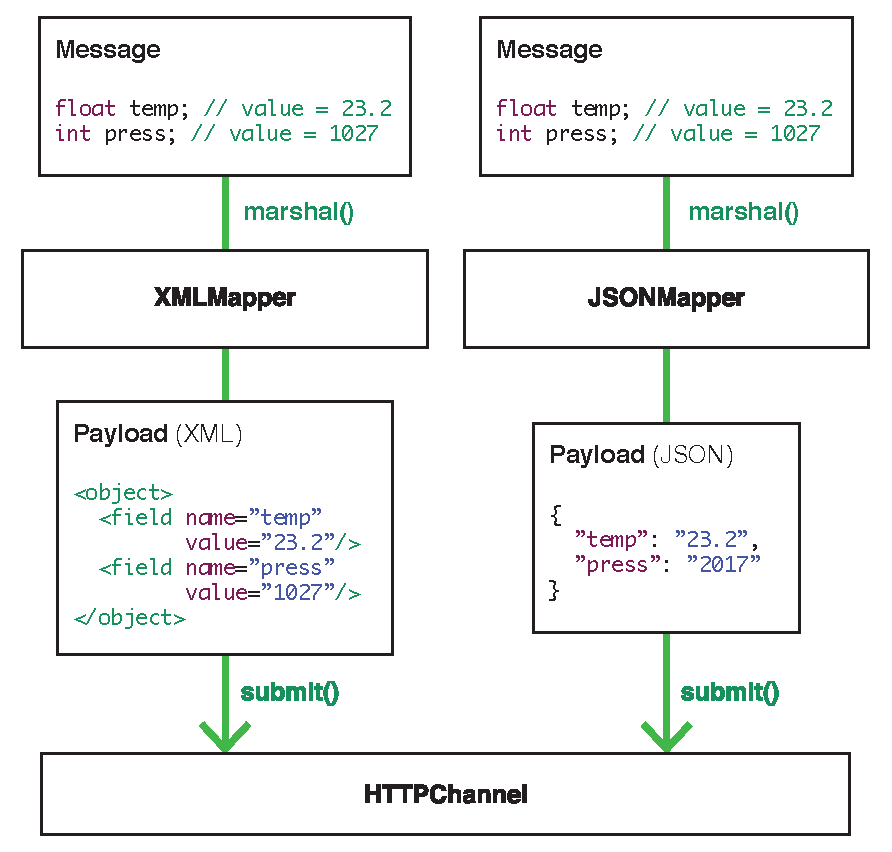
\includegraphics[scale=0.8]{imgs/mapper_channel.pdf}
    \caption{Using a single \texttt{Channel} to transmit data marshalled with
    different \texttt{Mapper}s}
    \label{fig:mapper_channel}
\end{figure}

Before this section comes to an end, it is worth putting into context the role
occupied by the \texttt{Mapper} inside the PerLa Middleware. The additional
decoupling provided by the \texttt{Mapper} builds over the pluggable
\texttt{Channel} interface, thus allowing the payload format to be selected
independently of the I/O stack.  This is an important characteristic of the
Middleware design, as even the simplest communication protocol usually requires
several \texttt{Message} structures, viz. several \texttt{Mapper}s, for
exchanging data between two endpoints.


\subsection{Creating Mappers and defining Message structures}

New \texttt{Mapper} objects are created by means of the \texttt{MapperFactory}
interface.

\lstset{language=Java}
\begin{lstlisting}[float,floatplacement=!hbt,caption=The Mapper Factory
interface,label={lst:mapperFactory}]
public interface MapperFactory {

    public Class<? extends MessageDescriptor>
        acceptedMessageDescriptorClass();

    public Mapper createMapper(MessageDescriptor descriptor,
        Map<String, Mapper> mapperMap, ClassPool classPool)
                    throws InvalidDeviceDescriptorException;

}
\end{lstlisting}

Its design follows the same concepts explained in previous sections; the
\texttt{acceptedMessageDescriptorClass()} method returns the type of
\texttt{MessageDescriptor} objects that can be used with the
\texttt{MapperFactory}, while the \texttt{createMapper()} method consumes a
\texttt{MessageDescriptor} to create a \texttt{Mapper}. However, differently
from all factory components described so far, the creation of a new object
calls for two additional parameters other than the descriptor itself: a
\texttt{ClassPool}, and a map of \texttt{Mapper}s. These extra items contain a
reference to previously built \texttt{Mapper}s, and can be used to check
whether nested \texttt{Message} fields are properly declared or not.

The \texttt{MapperFactory} interface is an additional extension point available
to PerLa users, and can be leveraged to introduce support for new binary
formats and information encoding schemes. As a consequence, every installation
of the Middleware will contain a wide variety of \texttt{MapperFactory}
implementations, each of which is dedicated to a single data format. Instances
of the previously introduced JSON and URL-Encoded mappers, for example, are
created by two distinct \texttt{MapperFactory} objects, namely
\texttt{JSONMapperFactory} and \texttt{URLEncodedMapperFactory}. This design is
a substantial improvement on the previous middleware architecture, as it
ensures that every \texttt{MapperFactory} object is responsible for managing
the quirks of only a single data format.

Moreover, every \texttt{MapperFactory} implementation is bundled with a custom
\texttt{MessageDescriptor} object, whose class name is exposed by the
aforementioned \texttt{acceptedMessageDescriptorClass()} method. The additional
complexity deriving from this design choice is more than made up for in type
safety and flexibility, as each different \texttt{MessageDescriptor} may be
implemented to closely represent the idiosyncratic characteristics of its
corresponding data format. A concrete example of this concept comes from the
\texttt{URLEncodedMessageDescriptor} class, which prevents the creation of
\texttt{Message}s that don't comply with the URL-encoded format by disallowing
non-primitive fields. Having multiple \texttt{MessageDescriptor}s also means
that different \texttt{Message}s are not forced to abide by the same set of
rules; the limits imposed on URL-encoded messages are not universal, and in
fact the \texttt{JSONMessageDescriptor} refrains from applying them.
Furthermore, \texttt{MessageDescriptor} objects can adopt a custom lexicon for
expressing the PerLa-specific concepts of \textit{message}, \textit{field} and
\textit{field type}. Take for example listings \ref{lst:jsonmessage} and
\ref{lst:urlencodedmessage}. These two XML snippets show how the vocabulary
employed in message declarations varies with the data format (field are dubbed
\textit{member} in JSON, and \textit{parameter} in URL-Encoded strings). Using
a terminology that best suits the actual data format makes \texttt{Message}
declarations idiomatic, reminiscent of the corresponding real-world objects and
therefore easier to use.

\lstset{language=XML}
\begin{lstlisting}[float,floatplacement=!hbt,caption={A compound JSON message
        declared using the JSONMessageDescriptor (XML notation). Note that the
        data type of all fields inside \texttt{weather} message is a reference
        to a previously declared \texttt{Message}.
},label={lst:jsonmessage}]

<js:object id="coord">
    <js:member name="lon" type="string"/>
    <js:member name="lat" type="string"/>
</js:object>

<js:object id="main">
        <js:member name="temp" type="float"/>
        <js:member name="pressure" type="float"/>
        <js:member name="humidity" type="float"/>
        <js:member name="temp_min" type="float"/>
        <js:member name="temp_max" type="float"/>
</js:object>

<js:object id="wind">
        <js:member name="speed" type="float"/>
        <js:member name="deg" type="float"/>
</js:object>

<js:object id="weather">
        <js:member name="coord" type="coord"/>
        <js:member name="main" type="main"/>
        <js:member name="wind" type="wind"/>
</js:object>

\end{lstlisting}


\lstset{language=XML}
\begin{lstlisting}[float,floatplacement=!hbt,caption={An URLEncoded message
declaration. Thanks to the custom \texttt{URLEncodedMessageDescriptor}, trying
to create a non-primitive field results in an exception. Note the custom
\texttt{format} attribute on the timestamp field, which is employed to define
the encoding format for dates and times},label={lst:urlencodedmessage}]

<ue:message id="urlencoded_message">
        <ue:parameter name="temperature" type="float"/>
        <ue:parameter name="pressure" type="float"/>
        <ue:parameter name="location" type="string"/>
        <ue:parameter name="key" qualifier="static" type="integer" value="5"/>
        <ue:parameter name="timestamp" type="timestamp" format="d MMM uuuu HH:mm"/>
</ue:message>

\end{lstlisting}


\subsection{Managing multiple message types}

It is not uncommon for a single device to communicate using multiple message
formats; developers may choose to encapsulate different information inside
different data structures, which the receiver must correctly identify to
decipher their contents. In such cases, every \texttt{Message} exchanged
between the two endpoints is tagged with a data type value, i.e., a common
field that advertises the type of information being transferred. This technique
is widespread among firmware developers, since it can be easily implemented
with most programming languages (C/C++ support it by design through
\texttt{tagged unions}).

The PerLa Middleware implements various techniques to cope with sensor nodes
that communicate using multiple message formats. First of all, only the data
structures that can actually be received are considered when unmarshalling a
byte stream; if under the current conditions a device only sends a subset of
its available message types, then the Middleware can immediately rule out the
unmatching ones. As it will be discussed later, a collection of expected data
formats is automatically curated by the \texttt{FPC} by cross-comparing
information excerpted from the Device Descriptor with the current device
status. It should be clear that this technique alone is not enough to cover all
practical use cases, as it falls short as soon as a device starts sending two
or more message varieties concurrenty; in such scenarios, PerLa needs to search
for clues that will help it recognize how the bytes being received are
structured. These clues take the form of \textit{static} fields. When faced
with an ambiguous situation, the \texttt{FPC} will try unmarshal the bytes
received into all expected data types. A congruency check will then be
performed on the resulting \texttt{Message}s: the data can be considered
correctly decoded only when all its static fields match the corresponding
Device Descriptor declaration. This methodology can be employed to interact
with sensor nodes that make use of tagged data structures. 


\section{Data management: Scripts}
\label{sec:components.script}

\texttt{Channel}s, \texttt{Payload}s, \texttt{Mapper}s and \texttt{Message}s
are the core components used by PerLa to exchange data with nodes of a
Pervasive System. They provide the supporting infrastructure through which
information can be serialized, transmitted and faithfully reconstructed at the
receiving endpoint. Taken together, these components implement an adaptable
transport layer, whose features can be tailored around each device connected to
the Middleware: combine a \texttt{HTTPChannel} with a \texttt{JSONMapper} to
obtain a network stack for RESTful services; swap the data layer with an
\texttt{XMLMapper} if the format changes; add a \texttt{ZigbeeChannel} and a
\texttt{StructMapper} to communicate with low-powered devices in a mesh
network. In spite of their individual capabilities, all these components are
not enough to glean information from a Sensor Network. The interaction with a
sensor node requires far more than a transport layer; in fact it can only occur
when data transfer operations follow a strict set of rules, i.e., an
\textit{application protocol}. \texttt{Channel}s, \texttt{Mapper}s and
\texttt{Message}s provide no more than the basic building blocks needed for the
interaction, but their use is to be tightly orchestrated before any purposeful
exchange of information can take place.

PerLa \textit{Script}s, just referred as \textit{Script}s in the remainder of
this document, implement the kind of structural scaffolding required to
organize a series of primitive data management operations into a
self-contained, reusable procedure. Their purpose in the PerLa Middleware is
twofold: first, to issue commands that conform to the specific protocols used
in a Pervasive Systems; second, to act as an impedance matcher between the
structured information collected from a sensor network and the record-oriented
output of an \texttt{FPC}. The PerLa scripting language is one of the most
distinctive features of the new Middleware design; a procedural programming
tool that can be used to complement and enrich the declarative nature of the
Device Descriptor. \textit{Script}s improve the reusability of all existing and
future Middleware components, as they can be used to adjust the output of a
computation before it's used as the input of another one.

\begin{figure}[h!]
    \centering
    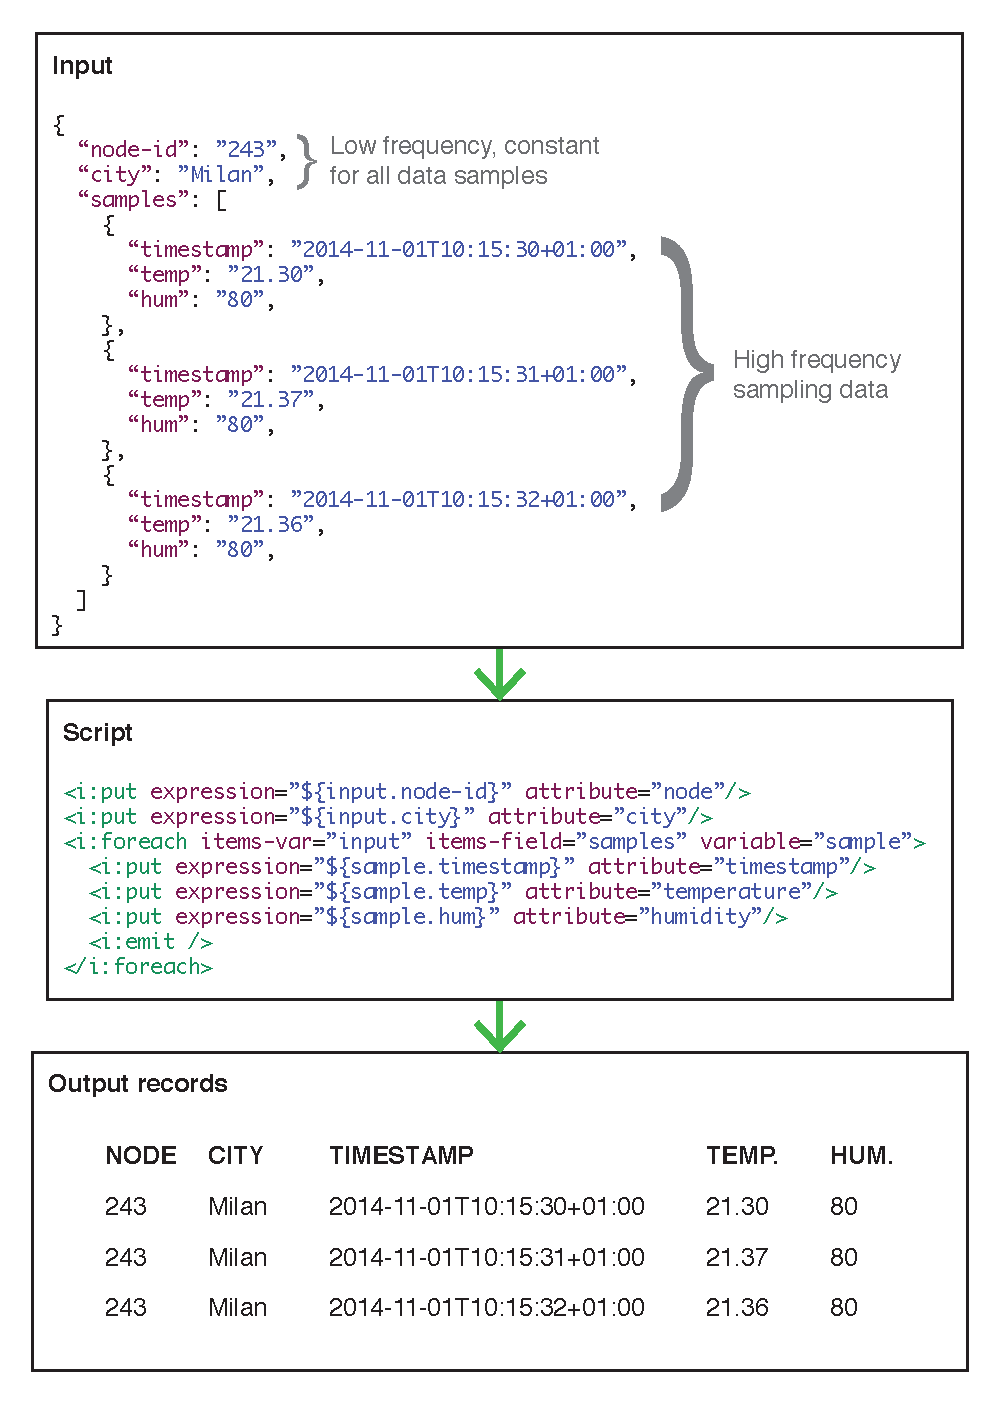
\includegraphics[scale=0.8]{imgs/script_unrolling.pdf}
    \caption{A script for unrolling the content of a JSON data structure}
    \label{fig:script_unrolling}
\end{figure}

An archetypal example of this concept is given in
figure~\ref{fig:script_unrolling}. This \textit{Script} solves a recurring
impedance matching problem: a device that stores multiple samples into a common
data structure, and sends them with a single transmission in order to conserve
battery power. The result of such aggregation can't be coerced into a sequence
of records as-is, as more often than not it contains a mixture of both high
frequency and low frequency information (and indeed it does in the current
example). The PerLa scripting language can be used to unroll the high frequency
content, complement it with the information that remains constant for all
samples, and output the resulting records one by one; all without having to
resort to a bespoken \texttt{Mapper} implementation, as it would prove
necessary if the former Middleware were used instead. Moreover, this same
script can be easily employed to handle similar aggregation patterns with
little or none modifications, as it doesn't depend on any particular
\texttt{Channel}, \texttt{Mapper} or \texttt{Message} implementation.

PerLa \textit{Scripts} are also used to address minor compatibility problems
that may arise when authoring new Device Descriptors; they can wrap an existing
Middleware component and adapt its behaviour to handle an unforseen usage
scenario, convert information between different units of measure, alter a
\texttt{Message} before it is sent to the intended recipient, or compute
aggregations. It is important to note that \textit{Scripts} are slower than
pure Java code; an excessive usage in data intensive, real-time applications
should be carefully avoided, as it may negatively affect the performance of the
entire Middleware. End users are therefore invited to thoroughly test and
benchmark their Device Descriptors to eliminate any potential bottleneck before
deployment.


\subsection{Anatomy of a PerLa Script}

PerLa \texttt{Script} is a full-fledged imperative programming language
composed of data management instructions, control flow statements and a
powerful expression language. Procedures written in PerLa \texttt{Script} are
processed by the \texttt{Script Engine}, a Middleware module that reads,
interprets and executes script instructions. Instructions are specified using a
proprietary XML syntax, specifically designed to allow PerLa \texttt{Scripts}
to be directly embedded in a Device Descriptor. Conflicts with potentially
similar XML tags and attributes are avoided through the
\texttt{http://perla.dei.org/device/instructions} namespace, which is commonly
associated with the ``\texttt{<i:}'' prefix. PerLa developers are invited to
follow this convention, as the use of a different namespace prefix may create
confusion among end users and future Device Descriptor maintainers. 

Every \texttt{Script} instruction is composed of a \textit{name}, a textual
property that identifies a specific type of computation, and a list of
\textit{parameters}, name-value pairs that can be used customize its runtime
behaviour. With the exception of the \texttt{submit} instruction, whose
unconventional characteristics are described in the remainder of this section,
instruction parameters are defined using the standard XML attribute syntax.
PerLa \texttt{Scripts} currently support two different types of parameters:
\textit{literals} and \textit{expressions}. Literals are simple textual strings
whose value is used as-is by the execution engine; they are commonly employed
to express constant concepts like variable names or immutable values.
Expressions, on the other hand, are combinations of variables, operators,
functions and constants, whose evaluation produces a result value. Differently
from literals, expressions are prefixed by the \$ sign and enclosed in curly
braces (\lstinline!${ ... }!); this cue is employed by the execution engine to
determine whether an instruction parameter has to be pre-processed or not prior
to being used. Expressions can be used to perform the following operations:

\begin{itemize}
        
    \item Arithmetic operations (sum, subtration, product, division, modulo)

    \item Logical operations (or, and, not)

    \item Comparisons (\lstinline$<, >, !=, <=, >=$)

    \item Access \texttt{Message} fields (dot operator). Multiple dot operators
        may be applied in succession to access a specific value buried inside a
        complex data structure (e.g., the expression
        \lstinline!${result.environment.temperature}! is used to traverse 3
        nesting levels).

    \item Retrieve \texttt{Script} arguments through the built-in \texttt{args}
        associative array. This feature can be leveraged to create parametric
        \texttt{Script}s that dynamically adapt to the user's requests.

\end{itemize}

Whether a certain parameter can be specified as a literal, as an expression, or
both, depends entirely on the instruction in which it is employed. This
information, along with other useful details regarding the \texttt{Script}
instructions currently available in PerLa, is available in the following
instruction compendium.

\subsubsection{\texttt{var} instruction}

\textbf{Description}

Declares a new variable. This instruction requires two mandatory parameters:

\begin{itemize}

    \item \textbf{name:} The variable name, namely a textual identifier used to
        reference the variable in later instructions. It must be unique in the
        scope of a single script.

    \item \textbf{type:} The type of data that can be stored inside the newly
        created variable. It can be set to one of the six PerLa primitive data
        types, or to a user-defined  message type.

\end{itemize}

\textbf{Usage examples}

Creates a new variable named \texttt{count} of primitive type \texttt{integer}.

\lstset{language=XML}
\begin{lstlisting}
<i:var name="count" type="integer"/>
\end{lstlisting}

Creates a new variable named \texttt{cmd} of complex type
\texttt{node\_command}, whose declaration is omitted for brevity reasons.

\lstset{language=XML}
\begin{lstlisting}
<i:var name="cmd" type="node_command"/>
\end{lstlisting}

\subsection{\texttt{set} instruction}

\textbf{Description}

Sets the contents of a variable to a new value. The optional \texttt{field}
parameter can be used whenever the user needs to modify a specific field of a
variable of complex type.

\begin{itemize}

    \item \textbf{variable:} Name of the variable to be modified.

    \item \textbf{field (optional):} An optional parameter that can be used to
        select the specific field to set in a variable of complex type.

    \item \textbf{value:} The new value of the variable. This parameter may
        either be a literal value or an expression.

\end{itemize}

\textbf{Usage examples}

Sets the previously defined \texttt{count} variable to the literal value \texttt{5}.

\lstset{language=XML}
\begin{lstlisting}
<i:set variable="count" value="5"/>
\end{lstlisting}

Sets the field \texttt{operation} of the previously defined \texttt{cmd}
variable to the literal value \texttt{sample}.

\lstset{language=XML}
\begin{lstlisting}
<i:set variable="cmd" field="operation" value="sample"/>
\end{lstlisting}

Converts a temperature reading from Celsius to Fahreheit degrees, and stores it
in the \texttt{temp\_f} field of a hypothetical variable named \texttt{result}.

\lstset{language=XML}
\begin{lstlisting}
<i:set variable="result" field="temp\_f"
    value="${result.temp\_c * 9/5 + 32}"/>
\end{lstlisting}

Deep copy. The contents of the source variable is accessed through the
\lstinline!${original}! expression.

\lstset{language=XML}
\begin{lstlisting}
<i:set variable="copy" value="${original}"/>
\end{lstlisting}


\subsubsection{\texttt{append} instruction}

\textbf{Description}

Appends a new element to the end of a list-qualified field.

\begin{itemize}

    \item \textbf{variable:} Name of the variable to be modified.
    
    \item \textbf{field:} Name of the field where the new value is to be
        appended.

    \item \textbf{value:} The new value to be inserted at the end of the list.
        This parameter may either be a literal value or an expression.

\end{itemize}

\textbf{Usage examples}

Appends a literal value to a list field.

\lstset{language=XML}
\begin{lstlisting}
<i:append variable="result" field="temp_list" value="5"/>
\end{lstlisting}


\subsubsection{\texttt{submit} instruction}

\textbf{Description}

Submits an \texttt{IORequest} on a \texttt{Channel}. This instruction supports
the following parameters:

\begin{itemize}

    \item \textbf{request:} Identifier of the \texttt{IORequest} to be
        submitted.

    \item \textbf{channel:} Identifier of the \texttt{Channel} on which the
        request has to be submitted

    \item \textbf{variable (optional):} Name of the variable used to store the
        result of the I/O operation. If present, the complementary
        \textbf{type} parameter must be set. It is important to note that the
        result variable is automatically declared by the \texttt{submit}
        instruction; therefore, the final user needs not to create it
        explicitly with a \texttt{var} instruction.

    \item \textbf{type (optional):} Type of the variable used to store the
        result of the I/O operation. Its presence is subordinated to the
        aforementioned \textbf{type} parameter.

\end{itemize}

\texttt{IORequest} parameters can be specified by supplying an appropriate list
of \texttt{param} XML tags, each of which must contain the name of the
parameter being set, and a reference to a variable containing the desired
parameter value (see the usage example section for further information).

\textbf{Usage examples}

Basic usage, submits the \texttt{start\_sampling} \texttt{IORequest} to a
\texttt{SerialChannel}. All information received during the I/O operation is
discarded since no result variable is specified.

\lstset{language=XML}
\begin{lstlisting}
<i:submit request="start_sampling" channel="serial"/>
\end{lstlisting}

Submits the \texttt{get\_data} \texttt{IORequest} to a \texttt{HTTPChannel}.
All bytes received from the remote server are stored in the \texttt{result}
variable.

\lstset{language=XML}
\begin{lstlisting}
<i:submit request="get_data" channel="http"
  variable="result" type="json_result"/>
\end{lstlisting}

Submits the \texttt{send\_command} \texttt{IORequest} to a
\texttt{SerialChannel}.  The \texttt{command} variable is set as an
\texttt{IORequest} parameter.

\lstset{language=XML}
\begin{lstlisting}
<i:submit request="get_data" channel="http">
  <i:param name="payload" variable="command"/>
</i:submit>
\end{lstlisting}


\subsubsection{\texttt{stop} instruction}

\textbf{Description}

Stops the \texttt{Script}. This instruction is usually employed in conjunction
with the \texttt{if} control structure to implement advanced halt conditions
based on data only available at runtime.

\textbf{Usage example}

Immediately stops the execution of the \texttt{Script}.

\lstset{language=XML}
\begin{lstlisting}
<i:stop/>
\end{lstlisting}

Guarded stop. Halts the execution of the \texttt{Script} only when a certain
condition holds true.

\lstset{language=XML}
\begin{lstlisting}
<i:if condition="${temp_c > 25}"> 
  <i:then>
    <i:stop/>
  </i:then>
</i:if>
\end{lstlisting}


\subsubsection{\texttt{error} instruction}

\textbf{Description}

Aborts the \texttt{Script}, signalling an abnormal execution condition. This
instruction must be supplied with a \textbf{message} parameter that indicates
the cause of failure. Similarly to the \texttt{stop} instruction,
\texttt{error} invocations are commonly guarded by an \texttt{if} control
structure to implement advanced error management behaviours.

\textbf{Usage examples}

\lstset{language=XML}
\begin{lstlisting}
<i:if condition="${humidity >= 0 && humidity <= 100}"> 
  <i:then>
    <i:put expression="${humidity}" attribute="humidity"/>
    <i:emit/>
    <i:stop/>
  </i:then>
  <i:else>
    <i:error message="humidity out of range"/>
  </i:else>
</i:if>
\end{lstlisting}


\subsubsection{\texttt{put} instruction}

\textbf{Description}

Adds a field into the staging area, viz. a temporary storage location used
for the incremental creation of new output records. This instruction requires
two mandatory parameters:

\begin{itemize}

    \item \textbf{attribute:} Name of the attribute corresponding to the value
        being added in the staging area. The purpose of this parameter is
        twofold: first, it defines the name through which the new data can be
        retrieved (record field names always correspond to device attribute
        names); second, it is used to confirm that the value being added in the
        staging area has the correct data type (record field types always
        correspond to device attribute types).

    \item \textbf{expression:} Value of the new record field.

\end{itemize}

This instruction is intended to be called multiple times in the lifetime of a
single \texttt{Script} execution, as a single \texttt{put} operation can only
be used to set one record field at a time. As soon as all the desired values
are ready, the content of the entired staging area can be flushed into a new
record by means of the \texttt{emit} instruction.

It is worth noting that the content of the staging area is not deleted once
\texttt{emit} is invoked. Though this may seem counterintuitive or even
undesirable, such behaviour allows for a simpler and more efficient management
of aggregated data. The ability to retain all field values set with previous
invocations of the \texttt{put} instruction is key to the example of
figure~\ref{fig:script_unrolling}, where low frequency information --- namely
the \textit{name-id} and the \textit{city} records --- is set only once, and
only the high-frequency samples are continuously replaced with new calls to the
\texttt{put} instruction. This optimization technique would not be possible if
the staging area were not provided with the aforementioned memory-retaining
mechanism.

\textbf{Usage Examples}

Refer to section~\ref{sec:emit_instruction} for combined usage examples of the
instructions \texttt{put} and \texttt{emit}.


\subsubsection{\texttt{emit} instruction}
\label{sec:emit_instruction}

\textbf{Description}

Creates a new record using the field values stored in the staging area. All
records created by the \texttt{emit} instruction are released to the user only
if the \texttt{Script} terminates without errors.

\textbf{Usage Examples}

Creates a record containing two literal fields.

\lstset{language=XML}
\begin{lstlisting}
<i:put attribute="temperature" expression="25"/>
<i:put attribute="humidity" expression="85"/>
<i:emit/>
\end{lstlisting}

Maps a flat data structure into a record. Differently from the previous
example, record values are dynamically read from the \texttt{sample} variable
hypothetically received from a remote sensor node.

\lstset{language=XML}
\begin{lstlisting}
<i:put attribute="temperature" expression="${sample.temperature}"/>
<i:put attribute="humidity" expression="${sample.humidity}"/>
<i:put attribute="timestamp" expression="${sample.timestamp}"/>
<i:emit/>
\end{lstlisting}

\texttt{Script} expressions can also be used to create new record values at
runtime. In the following code excerpt, a simple conversion formula is employed
to derive the \texttt{temp\_fahrenheit} record field from other information
sent by the sensor node.

\lstset{language=XML}
\begin{lstlisting}
<i:put attribute="temp_centigrade" expression="${sample.temp_cent}"/>
<i:put attribute="temp_fahrenheit"
  expression="${sample.temp_centigrade * 9/5 + 32}"}"/>
<i:put attribute="humidity" expression="${sample.humidity}"/>
<i:put attribute="timestamp" expression="${sample.timestamp}"/>
<i:emit/>
\end{lstlisting}

Looping over multiple samples stored in a list. The following example creates a
new record for each element contained in the \texttt{data.samples} field. 

\lstset{language=XML}
\begin{lstlisting}
<i:foreach items-var="data" items-field="samples" variable="sample">
  <i:put expression="${sample.timestamp}" attribute="timestamp"/>
  <i:put expression="${sample.temp}" attribute="temperature"/>
  <i:put expression="${sample.hum}" attribute="humidity"/>
  <i:emit/>
</i:foreach>
\end{lstlisting}

Exploiting the characteristic memory-retention feature of the \texttt{put}
instruction to efficiently combine high-frequency and low-frequency
information. Note that the \texttt{node} and \texttt{city} fields are staged
only once, while all other fast changing information requires the execution of
a \texttt{put} instruction for each list element.

\lstset{language=XML}
\begin{lstlisting}
<i:put expression="${input.node-id}" attribute="node"/>
<i:put expression="${input.city}" attribute="city"/>
<i:foreach items-var="input" items-field="samples" variable="sample">
  <i:put expression="${sample.timestamp}" attribute="timestamp"/>
  <i:put expression="${sample.temp}" attribute="temperature"/>
  <i:put expression="${sample.hum}" attribute="humidity"/>
<i:emit />
</i:foreach> 
\end{lstlising}

\subsubsection{\texttt{if} control structure}

\textbf{Description}

A conditional control structure for executing different texttt{Script} branches
depending on whether a user-specified \textbf{condition} expression evaluates
to true or false.

\textbf{Usage example}

If..then example. Sets the variable \texttt{alarm} to TRUE when the temperature
rises above 25\degree~C.

\lstset{language=XML}
\begin{lstlisting}
<i:if condition="${temp_c > 25}"> 
  <i:then>
    <i:set variable="alarm" value="true"/>
  </i:then>
</i:if>
\end{lstlisting}

If..then..else example. Sets the variable \texttt{tropical} to TRUE when the
temperature rises above 30\degree~C and the humidity is higher than 90\%, or
to false when the condition does not hold.

\lstset{language=XML}
\begin{lstlisting}
<i:if condition="${temp_c > 25 && hum > 90}"> 
  <i:then>
    <i:set variable="tropical" value="true"/>
  </i:then>
  <i:else>
    <i:set variable="tropical" value="true"/>
  </i:else>
</i:if>
\end{lstlisting}


\subsubsection{\texttt{foreach} control structure}

\textbf{Description}

A control structure for traversing list-qualified \texttt{Message} fields. It
can be used to repeat a given block of code for every element of a collection.
The \texttt{foreach} control structure supports the following parameters:

\begin{itemize}

    \item \textbf{items-var:} Name of the source variable.

    \item \textbf{items-field:} Name of the source field, namely the
        list-qualified field inside the \textbf{items-var} on which to loop
        over.

    \item \textbf{variable:} Name of the variable through which the current
        item is exposed.

    \item \textbf{index (optional):} Index of the current item.

\end{itemize}

\textbf{Usage examples}

Computing the average of all temperatures received from a remote sensor node.

\lstset{language=XML}
\begin{lstlisting}
<i:var name="count" type="integer"/>
<i:set variable="count" value="0"/> 
<i:var name="avg" type="float"/>
<i:set variable="avg" value="0"/>
<i:foreach items-var="data" items-field="samples" variable="sample">
  <i:set variable="avg" value="${avg + sample.temperature}"/>
  <i:set variable="count" value="${count + 1}"/>
</i:foreach>
<i:set variable="avg" value=""${avg / cont}"/>
\end{lstlisting}

\subsection{Script Engine architecture and execution model}

The \texttt{Script Engine} is a software component responsible for the
execution of PerLa \texttt{Scripts}. It is currently implemented as a program
interpreter that parses and executes an intermediate PerLa \texttt{Script}
representation generated by the \texttt{FPCFactory}, dubbed SIR (Script
Intermediate Representation). SIR programs are directed graphs, where each node
is an instruction, and each arc is a potential evolution of the program status;
thus, SIR-encoded \texttt{Scripts} can be run by simply traversing the source
data structure until a \texttt{stop} instruction is encountered, or an error is
thrown. Thanks to this intermediate representation, the \texttt{Script Engine}
architecture is lean and efficient; the core execution loop need not to be
concerned with the continuous interpretation of textual instructions or with
complex error-checking procedures, as these two operations are only performed
once, by the \texttt{FPCFactory}, when a \texttt{Script} is translated in its
corresponding SIR form. Moreover, as a result of the additional decoupling
provided by this intermediate code representation, the introduction of a new
PerLa \texttt{Script} format does not entail any modification to the
\texttt{Script Engine}, as long as a suitable SIR translator is provided for
the new syntax.

Once started, PerLa \texttt{Scripts} are sandboxed in a dedicated thread of
execution. For better isolation, the current status of each running
\texttt{Scrip} instance is stored inside a private \texttt{ExecutionContext}
object, which contains the following elements:

\begin{itemize}

    \item \textbf{Program Counter:} A reference to the current instruction;

    \item \textbf{Variable Map:} An associative array that stores the current
        value of all declared variables;

    \item \textbf{Record staging area:} Temporary working area used to create
        new records;

    \item \textbf{Output records:} List of records to be returned when the
        \texttt{stop} instruction is encountered. 

\end{itemize}

This design ensures that all changes a single \texttt{Script} makes to its
environment will remain private, and that its status won't be altered by any
other rogue routine.

The execution of a \texttt{Script} is always subordinated to an external event,
like the submission of a new user request or the arrival of information from a
sensing device. In particular, PerLa \texttt{Scripts} associated with the
management of sensor data tend to run frequently and for a relatively short
period of time, as their execution is triggered by each sample collected from
the sensing network. To better cope with such usage scenario, the
\texttt{Script Engine} implements a thread caching mechanism that reduces
memory usage and startup time by reclaiming the runtime environment of each
terminated \texttt{Script} and repurposing it for a new execution. This caching
technique greatly reduces the overall number of objects allocated by the Java
Virtual Machine, and guarantees that the overhead due to the initialization of
new \texttt{ExecutionContext} instances is shared between multiple
\texttt{Script} runs.


What do we have to say about this module?

- How scripts are executed: interpretation, flowchart with the process of
execution
- Optimization through thread pool and re-useable execution context
- Yielding instructions: How the submit instruction is managed

\section{Putting it all together: the FPC}

\subsection{Data access interface}

\subsection{Controlling the remote device}

\subsection{Scheduling mechanism}


\section{Device Descriptor and FPC Factory}

\subsection{The XML Device Descriptor}

\subsection{FPC Factory}

\subsection{Registry}

\subsection{Complete XML Device Descriptor examples}

		\chapter{Conclusions}

\section{Comparison with the classic architecture}

\section{Future work}

\subsection{Implementation of new plugins}

\subsection{Alternative Device Descriptor forms}

\subsection{Accessing FPC methods through HTTP}

	\appendix


\end{document}
